\documentclass{article}
\usepackage{palatino}  % Police Palatino
\usepackage[T1]{fontenc}
\usepackage[utf8]{inputenc}
\usepackage[a4paper, margin=2cm]{geometry}
\usepackage{graphicx}
\usepackage{amsmath, amssymb}
\usepackage{bm}
\usepackage{siunitx}
\usepackage{booktabs}
\usepackage{multirow}
\usepackage{float}
\usepackage{hyperref}
\usepackage{bookmark}
\usepackage[table,dvipsnames,svgnames,x11names]{xcolor}
\usepackage{tikz}
\usepackage{tikz-3dplot}
\usepackage{pgfplots}
\pgfplotsset{compat=1.18}
\usetikzlibrary{positioning, arrows.meta, shapes.geometric, shapes, arrows, decorations.pathreplacing, calc, 3d, patterns}
\usepackage[most]{tcolorbox}
\usepackage{caption}
\usepackage{enumitem}
\usepackage{titlesec}
\usepackage{pifont}
\usepackage{fancyvrb}
\usepackage{fvextra}
\usepackage{algorithm}
\usepackage{algorithmic}
\usepackage{listings}
\usepackage{textcomp}
\usepackage{setspace}
\usepackage{comment}  % AJOUT: Package nécessaire pour \begin{comment}...\end{comment}
\singlespacing

% ============================================================================
% CONFIGURATION DE LISTINGS POUR C++
% ============================================================================
\lstdefinestyle{cppstyle}{
    language=C++,
    basicstyle=\ttfamily\footnotesize,
    keywordstyle=\color{blue}\bfseries,
    commentstyle=\color{darkgreen},
    stringstyle=\color{red!70!black},
    numbers=left,
    numberstyle=\tiny\color{gray},
    numbersep=5pt,
    frame=single,
    breaklines=true,
    breakatwhitespace=true,
    showstringspaces=false,
    tabsize=4,
    captionpos=b,
    upquote=true,
    columns=fullflexible,
    keepspaces=true,
    literate=
        {á}{{\'a}}1 {é}{{\'e}}1 {í}{{\'i}}1 {ó}{{\'o}}1 {ú}{{\'u}}1
        {à}{{\`a}}1 {è}{{\`e}}1 {ì}{{\`i}}1 {ò}{{\`o}}1 {ù}{{\`u}}1
        {â}{{\^a}}1 {ê}{{\^e}}1 {î}{{\^i}}1 {ô}{{\^o}}1 {û}{{\^u}}1
        {ã}{{\~a}}1 {õ}{{\~o}}1 {ç}{{\c{c}}}1
}
\lstset{style=cppstyle}

% ============================================================================
% CONFIGURATION DES CAPTIONS
% ============================================================================
\captionsetup{font=footnotesize, labelfont=bf, textfont=it, skip=0pt}

% ============================================================================
% ESPACES
% ============================================================================
\setlength{\textfloatsep}{8pt plus 2pt minus 2pt}
\setlength{\floatsep}{8pt plus 2pt minus 2pt}
\setlength{\intextsep}{8pt plus 2pt minus 2pt}
\setlength{\abovecaptionskip}{4pt}
\setlength{\belowcaptionskip}{0pt}

\setlist[itemize]{itemsep=0pt, topsep=2pt, parsep=0pt, partopsep=0pt}
\setlist[enumerate]{itemsep=0pt, topsep=2pt, parsep=0pt, partopsep=0pt}

\titlespacing*{\section}{0pt}{2ex plus 1ex minus .2ex}{1ex plus .5ex minus .2ex}
\titlespacing*{\subsection}{0pt}{1.5ex plus .5ex minus .2ex}{0.7ex plus .3ex minus .1ex}

\setlength{\abovedisplayskip}{6pt}
\setlength{\belowdisplayskip}{6pt}
\setlength{\abovedisplayshortskip}{4pt}
\setlength{\belowdisplayshortskip}{4pt}

% ============================================================================
% COULEURS
% ============================================================================
\definecolor{headingblue}{RGB}{46,116,181}
\definecolor{Carnelian}{rgb}{0.7,0.11,0.11}
\definecolor{darkblue}{RGB}{0,51,102}
\definecolor{lightblue}{RGB}{220,235,255}
\definecolor{lightgreen}{RGB}{230,250,230}
\definecolor{lightorange}{RGB}{255,240,220}
\definecolor{lightred}{RGB}{255,230,230}
\definecolor{lightgray}{RGB}{245,245,245}
\definecolor{successgreen}{RGB}{39,174,96}
\definecolor{warningorange}{RGB}{243,156,18}
\definecolor{errorred}{RGB}{231,76,60}
\definecolor{infoblue}{RGB}{52,152,219}
\definecolor{methode1}{RGB}{70,130,180}
\definecolor{methode1bis}{RGB}{60,179,113}
\definecolor{methode2}{RGB}{255,140,0}
\definecolor{theoriecolor}{RGB}{0,100,180}
\definecolor{wpetg}{RGB}{34,139,34}
\definecolor{inox}{RGB}{192,192,192}
\definecolor{water}{RGB}{100,149,237}
\definecolor{watercolor}{RGB}{100,180,255}
\definecolor{source}{RGB}{255,215,0}
\definecolor{sourcecolor}{RGB}{255,100,100}
\definecolor{gamma}{RGB}{255,69,0}
\definecolor{gammacolor}{RGB}{255,200,0}
\definecolor{bismuth}{RGB}{180,100,160}
\definecolor{upstreamcolor}{RGB}{80,80,255}
\definecolor{downstreamcolor}{RGB}{255,80,80}
\definecolor{detectorcolor}{RGB}{100,200,100}
\definecolor{kermacolor}{RGB}{100,255,255}
\definecolor{aircolor}{RGB}{200,230,255}
\definecolor{conecolor}{RGB}{255,180,100}
\definecolor{envelopecolor}{RGB}{230,230,230}
\definecolor{slabcolor}{RGB}{255,230,100}
\definecolor{transmitcolor}{RGB}{46,204,113}
\definecolor{absorbcolor}{RGB}{231,76,60}
\definecolor{scattercolor}{RGB}{241,196,15}

\definecolor{darkgreen}{rgb}{0,0.6,0}
\definecolor{billeA}{RGB}{218,165,32}
\definecolor{billeB}{RGB}{205,92,92}
\definecolor{codegreen}{rgb}{0,0.6,0}
\definecolor{codegray}{rgb}{0.5,0.5,0.5}
\definecolor{codepurple}{rgb}{0.58,0,0.82}
\definecolor{backcolour}{rgb}{0.95,0.95,0.92}

% Définition des couleurs pour checkpoint
\definecolor{dnacolor}{RGB}{65,105,225}
\definecolor{atmcolor}{RGB}{220,20,60}
\definecolor{checkcolor}{RGB}{34,139,34}
\definecolor{deathcolor}{RGB}{139,0,0}
\definecolor{survivecolor}{RGB}{0,128,0}
\definecolor{lowdose}{RGB}{255,165,0}
\definecolor{highdose}{RGB}{138,43,226}
\definecolor{g1color}{RGB}{135,206,250}
\definecolor{scolor}{RGB}{144,238,144}
\definecolor{g2color}{RGB}{255,182,193}
\definecolor{mcolor}{RGB}{221,160,221}

% Définition des couleurs pour review
\definecolor{HRSpos}{RGB}{200,230,200}
\definecolor{HRSneg}{RGB}{255,200,200}
\definecolor{headerblue}{RGB}{70,130,180}

% Couleurs
\definecolor{atmcolor}{RGB}{70,130,180}
\definecolor{chk2color}{RGB}{255,140,0}
\definecolor{cdc25color}{RGB}{220,20,60}
\definecolor{cdk1color}{RGB}{50,205,50}
\definecolor{cyclincolor}{RGB}{147,112,219}
\definecolor{phosphocolor}{RGB}{255,200,0}
\definecolor{stopcolor}{RGB}{220,50,50}
\definecolor{gocolor}{RGB}{50,205,50}


% Couleurs
\definecolor{atmcolor}{RGB}{70,130,180}
\definecolor{atminactive}{RGB}{150,150,150}
\definecolor{atmactive}{RGB}{50,205,50}
\definecolor{dsbcolor}{RGB}{220,50,50}
\definecolor{phosphocolor}{RGB}{255,165,0}
\definecolor{dnacolor}{RGB}{100,149,237}


% ============================================================================
% COMMANDES PERSONNALISÉES
% ============================================================================
\newcommand{\codeTight}{\fontsize{8pt}{9pt}\selectfont}
\newcommand{\cmark}{\textcolor{successgreen}{\ding{51}}}
\newcommand{\xmark}{\textcolor{errorred}{\ding{55}}}
\newcommand{\wmark}{\textcolor{warningorange}{\ding{45}}}

% ============================================================================
% BOÎTES TCOLORBOX
% ============================================================================
\newtcolorbox{databox}[1]{
    colback=blue!5,
    colframe=blue!75!black,
    fonttitle=\bfseries,
    title=#1
}

\newtcolorbox{resultbox}[1]{
    colback=green!5,
    colframe=green!75!black,
    fonttitle=\bfseries,
    title=#1
}

\newtcolorbox{warningbox}[1]{
    colback=orange!5,
    colframe=orange!75!black,
    fonttitle=\bfseries,
    title=#1
}

% ============================================================================
% REDÉFINITION DES SECTIONS ET SUBSECTIONS ENCADRÉES
% ============================================================================

% Compteurs pour numérotation
\newcounter{coloredsection}
\newcounter{coloredsubsection}[coloredsection]
\newcounter{coloredsubsubsection}[coloredsubsection]

% Commande pour section encadrée orange
\newcommand{\sectionbox}[1]{%
    \refstepcounter{coloredsection}%
    \begin{tcolorbox}[
        colback=orange!20,
        colframe=orange!50!black,
        boxrule=0.5pt,
        arc=2mm
    ]
    {\Large\bfseries\color{blue} \thecoloredsection. #1}
    \end{tcolorbox}
    \addcontentsline{toc}{section}{\protect\numberline{\thecoloredsection}#1}
    \vspace{0.3cm}
}

% Commande pour subsection encadrée vert foncé
\newcommand{\subsectionbox}[1]{%
    \refstepcounter{coloredsubsection}%
    \begin{tcolorbox}[
        colback=green!10,
        colframe=green!50!black,
        boxrule=0.5pt,
        arc=2mm
    ]
    {\large\bfseries\color{green!40!black} \thecoloredsection.\thecoloredsubsection. #1}
    \end{tcolorbox}
    \addcontentsline{toc}{subsection}{\protect\numberline{\thecoloredsection.\thecoloredsubsection}#1}
    \vspace{0.2cm}
}

% Commande pour subsubsection encadrée Carnelian
\newcommand{\subsubsectionbox}[1]{%
    \refstepcounter{coloredsubsubsection}%
    \begin{tcolorbox}[
        colback=Carnelian!10,
        colframe=Carnelian!70!black,
        boxrule=0.5pt,
        arc=2mm
    ]
    {\normalsize\bfseries\color{Carnelian!70!black} \thecoloredsection.\thecoloredsubsection.\thecoloredsubsubsection. #1}
    \end{tcolorbox}
    \addcontentsline{toc}{subsubsection}{\protect\numberline{\thecoloredsection.\thecoloredsubsection.\thecoloredsubsubsection}#1}
    \vspace{0.15cm}
}

% === ENVIRONNEMENT KEYPOINT ===
\newenvironment{keypoint}
  {\begin{quotation}\itshape\bfseries}
  {\end{quotation}}


% ============================================================================
% DÉBUT DU DOCUMENT
% ============================================================================
\begin{document}

% ============================================================================
% TITRE PERSONNALISÉ
% ============================================================================
\begin{center}
    {\LARGE\bfseries\color{blue} Hypersensibilité Cellulaire aux Faibles Doses de Radiation}\\[0.3cm]
    {\large Phénomène HRS/IRR dans le Domaine des Centigrays}\\[0.2cm]
    {\large Mécanismes Moléculaires et Modèles Explicatifs}\\[0.3cm]
    {\normalsize Rapport de synthèse --- \today}
\end{center}

\vspace{0.5cm}

% ============================================================================
% ABSTRACT ENCADRÉ EN BLEU
% ============================================================================
\begin{tcolorbox}[
    colback=blue!5,
    colframe=blue!70!black,
    title=\textbf{Résumé},
    fonttitle=\color{white},
    colbacktitle=blue!70!black,
    arc=3mm,
    boxrule=1pt
]
\noindent L'hyper-radiosensibilité aux faibles doses (\textbf{HRS}) décrit un phénomène par lequel les cellules présentent une sensibilité excessive à de petites doses uniques de rayonnement ionisant, typiquement inférieures à 20--50~cGy selon la lignée cellulaire.\newline
Ce phénomène n'est pas prédit par l'extrapolation rétrograde de la réponse de survie cellulaire à partir des doses plus élevées utilisant le modèle linéaire-quadratique (\textbf{LQ}) standard.
\end{tcolorbox}

\vspace{0.5cm}

\tableofcontents

\newpage

%==============================================================================
\normalsize 
\sectionbox{Introduction}
\footnotesize 
%==============================================================================

\normalsize 
\subsectionbox{Caractérisation expérimentale du phénomène HRS/IRR}
\footnotesize 

\begin{tcolorbox}[
    colback=blue!5,
    colframe=blue!70!black,
    fonttitle=\color{white},
    colbacktitle=blue!70!black,
    arc=3mm,
    boxrule=1pt
]
\footnotesize L'\textbf{HRS} se manifeste par une pente initiale de la courbe de survie (\normalsize$\bm{\alpha_s}$\footnotesize) significativement plus élevée que celle observée à doses plus importantes (\normalsize$\bm{\alpha_r}$\footnotesize), avec un rapport $\normalsize\bm{\alpha_s}/\bm{\alpha_r}\footnotesize$ typiquement compris entre 2 et 5.
\end{tcolorbox}

\medskip

\footnotesize
\noindent À mesure que la dose augmente au-delà d'environ 20--40~cGy, on observe une augmentation de la radiorésistance (\textbf{IRR}) jusqu'à ce que, au-delà d'environ 1~Gy, la radiorésistance soit maximale et que la survie cellulaire suive la courbe descendante habituelle décrite par le modèle \textbf{LQ}.

% =============================================================================
% Skov 1999 FIGURE 1 : Structure HRS/IRR
% =============================================================================
\begin{figure}[h!]
\centering
\includegraphics[scale=1.5]{Figures/Figure1_Skov_1999.png}
\captionsetup{labelformat=empty, font=small}
\caption{\textbf{Structure stylisée de la courbe d'$\bm{IRR/HRS}$.} La structure anormale aux faibles doses : l'$\bm{HRS}$ (jusqu'à environ 0,25~Gy) est suivie d'une radiorésistance accrue ($\bm{IRR}$, jusqu'à environ 1~Gy). Cette courbe stylisée représente une lignée cellulaire de mammifère avec une $\bm{IRR}$ importante. $\bm{LQ}$ : L'ajustement linéaire-quadratique ($\bm{LQ}$ : $-\ln \bm{S} = \bm{\alpha} \bm{D} + \bm{\beta} \bm{}D^2$) est représenté par la ligne pointillée. Le « déficit » par rapport à l'ajustement $\bm{LQ}$ est la zone hachuré. Le $\bm{SF2}$ est la survie à 2~Gy, utilisée par de nombreux groupes pour décrire la radiosensibilité intrinsèque. La ligne pointillée indique la survie dans les cellules où il n'y a pas d'$\bm{IRR}$ (lignées sensibles, neutrons, développement de l'$\bm{IRR}$ inhibé par un sensibilisateur), suivant l'$\bm{HRS}$ initiale. \textbf{Amorçage} : Les cellules qui ont été « amorcées », par exemple par une petite dose de radiation, suivie d'un temps pour produire la réponse (généralement 4--6~h), ont perdu l'$\bm{HRS}$, c'est-à-dire que la réponse aux doses de défi est similaire à l'ajustement $\bm{LQ}$.}
\end{figure}


%==============================================================================
\normalsize 
\sectionbox{Historique}
\footnotesize 
%==============================================================================

\noindent Le phénomène a d'abord été observé \textit{in vivo} par Joiner et Johns en 1988~\cite{Joiner1988} dans des études sur les dommages rénaux chez la souris.\newline
\noindent La première démonstration \textit{in vitro} a été réalisée par Marples et Joiner en 1993~\cite{Marples1993} sur les cellules V79 de hamster chinois, où ils ont montré que l'effet par unité de dose augmentait d'un facteur $\sim$2, passant de 0,19~Gy$^{-1}$ à 1~Gy à 0,37~Gy$^{-1}$ à 0,1~Gy.\par
\medskip

%------------------------------------------------------------------------------
\normalsize 
\subsectionbox{Premi\`eres \'etudes in vitro sur lign\'ees cellulaires (1993--1997)}
\footnotesize 
%------------------------------------------------------------------------------

\begin{enumerate}
\setcounter{enumi}{1}
\item \footnotesize \hyperref[sec:resume2]{\color{blue}\textbf{Marples B, Joiner MC (1993)}\color{black}}.\ \\
\textbf{\textit{The response of Chinese hamster V79 cells to low radiation doses: evidence of enhanced sensitivity of the whole cell population.}}\\
Radiation Research, 133(1):41-51.\\
\scriptsize \url{https://pubmed.ncbi.nlm.nih.gov/8434112/}\\

\item \footnotesize \hyperref[sec:resume3]{\color{blue}\textbf{Lambin P, Marples B, Fertil B, Malaise EP, Joiner MC (1993)}\color{black}}.\ \\
\textbf{\textit{Hypersensitivity of a human tumour cell line to very low radiation doses.}}\\
International Journal of Radiation Biology, 63:639-650.\\
\scriptsize \url{https://pubmed.ncbi.nlm.nih.gov/8099110/}//

\item \footnotesize \hyperref[sec:resume4]{\color{blue}\textbf{Malaise EP, Lambin P, Joiner MC (1994)}\color{black}}.\ \\
\footnotesize \textbf{\textit{Radiosensitivity of human cell lines to small doses. Are there some clinical implications?}}\\
\footnotesize Radiation Research, 138(1 Suppl):S25-27.\\
\scriptsize \url{https://pubmed.ncbi.nlm.nih.gov/8146319/}\\

\item \footnotesize \hyperref[sec:resume5]{\color{blue}\textbf{Lambin P, Fertil B, Malaise EP, Joiner MC (1994)}\color{black}}.\ \\
\footnotesize \textbf{\textit{Multiphasic Survival Curves for Cells of Human Tumor Cell Lines: Induced Repair or Hypersensitive Subpopulation?}}\\
\footnotesize Radiation Research, 138(1 Suppl):S32-S36.\\
\scriptsize \url{https://www.jstor.org/stable/3578756}\\

\item \footnotesize \hyperref[sec:resume6]{\color{blue}\textbf{Wouters BG, Skarsgard LDb(1994)}\color{black}}.\ \\
\footnotesize \textbf{\textit{The response of a human tumor cell line to low radiation doses: Evidence of enhanced sensitivity.}}\\
\footnotesize Radiation Research, 138(1 Suppl):S76-S80.\\
\scriptsize \url{https://pubmed.ncbi.nlm.nih.gov/8146333/}\\

\item \footnotesize \hyperref[sec:resume7]{\color{blue}\textbf{Marples B, Adomat H, Koch CJ, Skov KA (1996)}\color{black}}.\ \\
\footnotesize \textbf{\textit{Response of V79 cells to low doses of X-rays and negative pi-mesons: Clonogenic survival and DNA strand breaks.}}\\
\footnotesize International Journal of Radiation Biology, 70(4):429-436.\\
\scriptsize \url{https://pubmed.ncbi.nlm.nih.gov/8862454/}\\

\item \footnotesize \hyperref[sec:resume8]{\color{blue}\textbf{Wouters BG, Sy AM, Skarsgard LD (1996)}\color{black}}.\ \\
\footnotesize \textbf{\textit{Low-Dose Hypersensitivity and Increased Radioresistance in a Panel of Human Tumor Cell Lines with Different Radiosensitivity.}}\\
\footnotesize Radiation Research, 146(4):399-413.\\
\scriptsize \url{https://pubmed.ncbi.nlm.nih.gov/8927712/}\\

\item  \footnotesize \hyperref[sec:resume9]{\color{blue}\textbf{Skarsgard LD, Skwarchuk MW, Wouters BG, Durand RE (1996)}\color{black}}.\ \\
\footnotesize \textbf{\textit{Substructure in the radiation survival response at low dose in cells of human tumor cell lines.}}\\
\footnotesize Radiation Research, 146(4):388-398.\\
\scriptsize \url{https://pubmed.ncbi.nlm.nih.gov/8927711/}\\

\item  \footnotesize  \hyperref[sec:resume10]{\color{blue}\textbf{Joiner MC, Lambin P, Malaise EP, Robson T, Arrand JE, Skov KA, Marples B (1996)}\color{black}}.\ \\
\footnotesize \textbf{\textit{Hypersensitivity to very-low single radiation doses: its relationship to the adaptive response and induced radioresistance.}}\\
\footnotesize Mutation Research, 358(2):171-183.\\
\scriptsize \url{https://pubmed.ncbi.nlm.nih.gov/8946022/}\\

\item  \footnotesize  \hyperref[sec:resume11]{\color{blue}\textbf{Marples B, Lambin P, Skov KA, Joiner MC (1997)}\color{black}}.\  \\
\footnotesize  \textbf{\textit{Low dose hyper-radiosensitivity and increased radioresistance in mammalian cells.}}\\
\footnotesize  International Journal of Radiation Biology, 71(6):721-735.\\
\scriptsize \url{https://pubmed.ncbi.nlm.nih.gov/9246186/}\\

\item  \footnotesize \hyperref[sec:resume12]{\color{blue}\textbf{Wouters BG, Skarsgard LD (1997)}\color{black}}.\  \\
\footnotesize \textbf{\textit{Low-dose radiation sensitivity and induced radioresistance to cell killing in HT-29 cells is distinct from the `adaptive response' and cannot be explained by a subpopulation of sensitive cells.}}\\
\footnotesize Radiation Research, 148(5):435-442.\\
\scriptsize \url{https://pubmed.ncbi.nlm.nih.gov/9355868/}

\end{enumerate}





%------------------------------------------------------------------------------
\normalsize 
\subsectionbox{Premi\`eres \'Etudes sur des lign\'ees spécifiques (1999--2004)}
\footnotesize 
%------------------------------------------------------------------------------


%------------------------------------------------------------------------------
\normalsize 
\subsectionbox{Publications récentes (2020--2025)}
\footnotesize 
%------------------------------------------------------------------------------






\newpage

%==============================================================================
\normalsize 
\sectionbox{Présentation globale de l'HRS/IRR}
\footnotesize 
%==============================================================================

\noindent Il existe maintenant des données sur les réponses à très faibles doses de plus de 46 lignées cellulaires humaines différentes, obtenues en utilisant à la fois des techniques de $\bm{FACS}$ et de localisation cellulaire microscopique.\newline
\begin{tcolorbox}[
    colback=Carnelian!5,
    colframe=Carnelian,
    coltitle=white,
    fonttitle=\bfseries\large,
    title={FACS (Fluorescence-Activated Cell Sorter)},
    arc=3mm,
    boxrule=2pt,
    left=10pt,
    right=10pt,
    top=10pt,
    bottom=10pt
]

\noindent Le $\bm{FACS}$ est un appareil qui permet de \textbf{trier des cellules une par une} en utilisant un faisceau laser.

\vspace{0.5em}
\textcolor{Carnelian}{\textbf{Principe simplifié :}}
\begin{enumerate}
    \item Les cellules passent en file indienne dans un flux liquide très fin
    \item Un laser analyse chaque cellule individuellement
    \item L'appareil peut détecter et compter précisément chaque cellule
    \item Il dépose ensuite un \textbf{nombre exact} de cellules dans chaque puits de culture
\end{enumerate}

\vspace{0.5em}
\textcolor{Carnelian}{\textbf{Pourquoi c'est important pour l'$\bm{HRS}$ ?}}
\noindent Pour mesurer la survie cellulaire à \textbf{très faibles doses} (< 0.1 Gy), il faut une précision extrême :
\begin{itemize}
    \item \textbf{Méthodes classiques :} on pipette $\sim$100 cellules, mais ça peut être 80 ou 120 $\rightarrow$ erreur de $\pm$20\%
    \item \textbf{Avec le $\bm{FACS}$ :} on dépose \textbf{exactement} 100 cellules $\rightarrow$ erreur minimale
\end{itemize}
\noindent Cette précision est \textbf{essentielle} car à faibles doses, la survie est proche de 100\%. Une petite erreur sur le nombre initial de cellules fausserait complètement les résultats.
\vspace{0.5em}

\textcolor{Carnelian}{\textbf{Alternative :}}
\noindent Le \textbf{balayage microscopique} (\textit{microscopic scanning}) : on dépose les cellules normalement, puis on les compte une par une au microscope avant l'irradiation.
\vspace{0.3em}
\hfill\textit{\small Ces deux méthodes ont permis de révéler le phénomène HRS dans les années 1990-2000.}

\end{tcolorbox}

\noindent L'hyper-radiosensibilité à faible dose dans les cellules humaines a maintenant été bien documentée par différents laboratoires utilisant différentes techniques d'essai et différentes conditions de croissance cellulaire, de manipulation et d'irradiation\newline

\noindent La Figure (\ref{Figure1_Joiner_1997}) illustre l'$\bm{HRS/IRR}$ dans les cellules de gliome humain $\bm{T98G}$. Le phénomène est généralement plus prononcé dans les lignées cellulaires humaines que dans les cellules $\bm{V79}$, et la réduction beaucoup plus abrupte de la survie cellulaire aux faibles doses par rapport aux doses élevées est clairement visible. Cette comparaison est indiquée dans la Figure (\ref{Figure1_Joiner_1997}) par les pentes $\bm{\alpha_s}$ et $\bm{\alpha_r}$, qui sont des paramètres de sensibilité dans l'équation mathématique de réparation induite ($\bm{IR}$) utilisée pour modéliser ces types de données, comme le montre la ligne continue. Le modèle linéaire-quadratique sous-estime substantiellement l'effet des faibles doses de radiation.

\begin{figure}[h!]
\centering
\includegraphics[scale=0.5]{Figures/Figure1_Joiner_1997.png}
\label{Figure1_Joiner_1997}
\caption{\textbf{Survie des cellules de gliome humain $\bm{T98G}$ asynchrones irradiées avec des rayons X de 240 kVp, mesurée en utilisant le protocole de tri cellulaire. Chaque point de données représente 10--12 mesures. Les lignes continues et en pointillés montrent les ajustements des modèles de réparation induite ($\bm{IR}$) et linéaire-quadratique ($\bm{LQ}$), respectivement. Aux doses inférieures à 1 Gy, le modèle $\bm{LQ}$, utilisant une pente initiale $\bm{\alpha_r}$, sous-estime substantiellement l'effet de l'irradiation, et ce domaine est mieux décrit par le modèle $\bm{IR}$ utilisant une pente initiale beaucoup plus raide $\bm{\alpha_s}$}}
\end{figure}

\subsectionbox{Base de données expérimentales}

\noindent Fin 2025, l'étude de $\bm{HRS/IRR}$ est basée sur plus de 46 publications et 101 jeux de données identifiés dans la littérature (Polgár et al., 2022 \cite{}).\newline
\noindent Une base de données numérisée des courbes de survie $\bm{HRS/IR}$ est disponible sur $\bm{STORED}$ :\textbf{URL :} \url{https://storedb.org/}\newline

\noindent Cette base contient les données brutes de 101 jeux de données provenant de 46 publications, permettant la méta-analyse et la validation de modèles biophysiques.

\noindent \textbf{Légende des tableaux :}
\begin{itemize}
    \item \colorbox{HRSpos}{Vert} = $\bm{HRS}$ positive (phénomène observé)
    \item \colorbox{HRSneg}{Rouge} = $\bm{HRS}$ négative (pas de phénomène observé)
    \item $\bm{\alpha_s}$ = pente initiale (région $\bm{HRS}$)
    \item $\bm{\alpha_r}$ = pente extrapolée des hautes doses
    \item $\bm{SF2}$ = Fraction survivante à 2 Gy
\end{itemize}

\subsectionbox{Lignées Cellulaires de Hamster}

\subsubsectionbox{V79 - Fibroblastes de Hamster Chinois}
La lignée $\bm{V79}$ est la première lignée de mammifères dans laquelle l'HRS/IRR a été clairement caractérisée (Marples \& Joiner, 1993[\cite{Marples1993}]).

\begin{center}
\begin{tabular}{|l|c|c|c|c|l|}
\hline
\rowcolor{headerblue}
\footnotesize \textcolor{white}{\textbf{Lignée}}&\footnotesize \textcolor{white}{\textbf{$\bm{HRS}$}}&\footnotesize \textcolor{white}{\textbf{$\bm{\alpha_s}/\bm{\alpha_r}$}}&\footnotesize \textcolor{white}{\textbf{$\bm{SF2}$}}&\footnotesize \textcolor{white}{\textbf{Rayonnement}}&\footnotesize  \textcolor{white}{\textbf{Référence}} \\
\hline
\rowcolor{HRSpos}
\footnotesize $\bm{V79}$ (aérobie)&\footnotesize +&\footnotesize 5-10&\footnotesize 0.65&\footnotesize Rayons X&\footnotesize Marples 1993 [\cite{Marples1993}]\\
\rowcolor{HRSpos}
\footnotesize $\bm{V79}$ (hypoxie)&\footnotesize +&\footnotesize $\sim$5&\footnotesize 0.85&\footnotesize Rayons X&\footnotesize Marples 1993 [\cite{Marples1993}]\\
\rowcolor{HRSpos}
\footnotesize $\bm{V79-379A}$ &\footnotesize + &\footnotesize --& --&\footnotesize $\pi$-mésons&\footnotesize Marples 1996 [\cite{Marples1996}]\\
\rowcolor{HRSneg}
\footnotesize $\bm{V79}$ &\footnotesize --&\footnotesize 1&\footnotesize --&\footnotesize Neutrons haut $\bm{TEL}$&\footnotesize Marples 1993 [\cite{Marples1993}]\\
\rowcolor{HRSpos}
\footnotesize $\bm{V79}$ &\footnotesize +&\footnotesize --&\footnotesize --&\footnotesize $^4$He$^{2+}$ (58.9 keV/$\mu$m)&\footnotesize 2002 [\cite{}]\\
\hline
\end{tabular}
\end{center}

\subsubsectionbox{Mutants de Réparation de l'ADN (Hamster)}

\begin{center}
\begin{tabular}{|l|l|c|c|l|}
\hline
\rowcolor{headerblue}
\footnotesize \textcolor{white}{\textbf{Lignée}}&\footnotesize \textcolor{white}{\textbf{Déficience}}&\footnotesize \textcolor{white}{\textbf{$\bm{HRS}$}}&\footnotesize \textcolor{white}{\textbf{$\bm{IRR}$}}&\footnotesize \textcolor{white}{\textbf{Référence}}\\
\hline
\rowcolor{HRSneg}
\footnotesize $\bm{XR-V15B}$&\footnotesize Ku80 ($\bm{NHEJ}$)&\footnotesize +&\footnotesize --&\footnotesize Skov 1994 [\cite{}]\\
\rowcolor{HRSneg}
\footnotesize $\bm{xrs5}$&\footnotesize Ku80 ($\bm{NHEJ}$)&\footnotesize+&\footnotesize --&\footnotesize Skov 1994 [\cite{}]\\
\rowcolor{HRSneg}
\footnotesize $\bm{UV-20}$&\footnotesize $\bm{NER}$ (excision nucléotides)&\footnotesize Exp.&\footnotesize --&\footnotesize Skov 1994 [\cite{}]\\
\rowcolor{HRSpos}
\footnotesize $\bm{EM9}$&\footnotesize $\bm{BER}$ (excision bases)&\footnotesize +&\footnotesize +&\footnotesize Skov 1994 [\cite{}]\\
\rowcolor{HRSpos}
\footnotesize $\bm{CHO-K1}$&\footnotesize Type sauvage&\footnotesize +&\footnotesize +&\footnotesize  Référence\\
\rowcolor{HRSneg}
\footnotesize $\bm{irs1SF}$&\footnotesize Recombinaison $\bm{HR}$&\footnotesize +&\footnotesize -- &\footnotesize Rothkamm 2003 [\cite{}]\\
\rowcolor{HRSneg}
\footnotesize $\bm{V3}$&\footnotesize $\bm{DNA-PKcs}$&\footnotesize +&\footnotesize --&\footnotesize Rothkamm 2003 [\cite{}]\\
\hline
\end{tabular}
\end{center}

\begin{tcolorbox}[colback=blue!5,colframe=blue,title=\textbf{Remarque}]
\noindent Les cellules déficientes en $\bm{NHEJ}$ ($\bm{Ku80}$, $\bm{DNA-PKcs}$) montrent l'$\bm{HRS}$ mais pas l'$\bm{IRR}$, suggérant que la voie $\bm{DNA-PK}$ est essentielle pour le développement de la radiorésistance induite
\end{tcolorbox}

\subsectionbox{Lignées Cellulaires Humaines - Gliomes}

\noindent Les gliomes représentent l'un des types tumoraux les plus étudiés pour l'$\bm{HRS}$/$\bm{IRR}$ en raison de leur radiorésistance clinique.

\begin{table}[h!]
\centering
\caption{\footnotesize Lignées cellulaires de gliomes testées pour $\bm{HRS}$/$\bm{IRR}$}
\begin{tabular}{|l|c|c|c|c|l|}
\hline
\rowcolor{headerblue}
\footnotesize \textcolor{white}{\textbf{Lignée}}&\footnotesize \textcolor{white}{\textbf{$\bm{HRS}$}}& \footnotesize \textcolor{white}{\textbf{$\bm{\alpha_s}$ (Gy$^{-1}$)}}&\footnotesize \textcolor{white}{\textbf{$\bm{\alpha_s}/\bm{\alpha_r}$}}&\footnotesize \textcolor{white}{\textbf{$\bm{SF2}$}}&\footnotesize \textcolor{white}{\textbf{Référence}} \\
\hline
\rowcolor{HRSpos}
\footnotesize $\bm{T98G}$& +&\footnotesize 2.5-4.0&\footnotesize 8-15& 0.58-0.65 &\footnotesize Short 1999 \cite{}, Joiner 2001 \cite{Joiner2001}\\
\rowcolor{HRSneg}
\footnotesize $\bm{U373}$& --&\footnotesize $\sim\bm{\alpha_r}$&\footnotesize  $\sim$1 & 0.63&\footnotesize Short 1999 \cite{}\\
\rowcolor{HRSpos}
\footnotesize $\bm{U87}$ (U87MG)&\footnotesize +&\footnotesize --&\footnotesize >5& 0.55&\footnotesize Short 1999 \cite{}\\
\rowcolor{HRSpos}
\footnotesize $\bm{U138MG}$&\footnotesize +&\footnotesize --&\footnotesize --&\footnotesize --&\footnotesize Martin 2013 \cite{}\\
\rowcolor{HRSpos}
\footnotesize $\bm{A7}$&\footnotesize  +&\footnotesize >2 &\footnotesize >10& 0.62&\footnotesize Short 1999 \cite{}\\
\rowcolor{HRSpos}
\footnotesize $\bm{HGL21}$&\footnotesize +&\footnotesize >2 &\footnotesize >8& 0.58&\footnotesize Short 1999 \cite{}\\
\rowcolor{HRSneg}
\footnotesize $\bm{MO59J}$&\footnotesize --&\footnotesize -- &\footnotesize --&\footnotesize très bas & $\bm{DNA-PKcs}$ déficient\\
\rowcolor{HRSpos}
\footnotesize $\bm{MO59}$K&\footnotesize +&\footnotesize -- &\footnotesize --&\footnotesize --&\footnotesize $\bm{DNA-PKcs}$ compétent\\
\hline
\end{tabular}
\end{table}

\subsectionbox{Lignées Cellulaires Humaines - Carcinomes}

\subsubsectionbox{Carcinome Colorectal}

\begin{center}
\begin{tabular}{|l|c|c|c|c|l|}
\hline
\rowcolor{headerblue}
\footnotesize \textcolor{white}{\textbf{Lignée}}&\footnotesize \textcolor{white}{\textbf{$\bm{HRS}$}}&\footnotesize \textcolor{white}{\textbf{$\bm{\alpha_s}/\bm{\alpha_r}$}}&\footnotesize \textcolor{white}{\textbf{$\bm{SF2}$}}&\footnotesize \textcolor{white}{\textbf{Notes}}&\footnotesize  \textcolor{white}{\textbf{Référence}} \\
\hline
\rowcolor{HRSpos}
\footnotesize $\bm{HT29}$ &\footnotesize + &\footnotesize 5-8 &\footnotesize 0.55-0.60 &\footnotesize Bien documentée&\footnotesize Wouters 1996 \cite{}, 1997 \cite{}\\
\rowcolor{HRSneg}
\footnotesize $\bm{SW48}$ &\footnotesize --&\footnotesize $\sim$1 &\footnotesize  0.25-0.30&\footnotesize Très radiosensible &\footnotesize  Lambin 1996 \cite{}\\
\rowcolor{HRSpos}
\footnotesize $\bm{DLD-1}$ &\footnotesize +&\footnotesize -- &\footnotesize --&\footnotesize -- &\footnotesize Andaur 2018 \cite{}\\
\hline
\end{tabular}
\end{center}

\subsubsectionbox{Carcinome de la Vessie}

\begin{center}
\begin{tabular}{|l|c|c|c|l|}
\hline
\rowcolor{headerblue}
\footnotesize \textcolor{white}{\textbf{Lignée}}&\footnotesize \textcolor{white}{\textbf{$\bm{HRS}$}}&\footnotesize \textcolor{white}{\textbf{$\alpha_s/\alpha_r$}}&\footnotesize \textcolor{white}{\textbf{$\bm{SF2}$}}&\footnotesize  \textcolor{white}{\textbf{Référence}} \\
\hline
\rowcolor{HRSpos}
\footnotesize $\bm{RT112}$&\footnotesize + &\footnotesize 5-7&\footnotesize 0.50-0.55&\footnotesize Lambin 1994 \cite{}\\
\rowcolor{HRSpos}
\footnotesize $\bm{UM-UC-3}$&\footnotesize + &\footnotesize --&\footnotesize --&\footnotesize Joiner 2001 \cite{Joiner2001}\\
\hline
\end{tabular}
\end{center}

\subsubsectionbox{Carcinome de la Prostate}

\begin{center}
\begin{tabular}{|l|c|c|c|l|}
\hline
\rowcolor{headerblue}
\footnotesize \textcolor{white}{\textbf{Lignée}}&\footnotesize \textcolor{white}{\textbf{$\bm{HRS}$}}&\footnotesize \textcolor{white}{\textbf{$\bm{\alpha_s}/\bm{\alpha_r}$}}&\footnotesize \textcolor{white}{\textbf{$\bm{SF2}$}}&\footnotesize \textcolor{white}{\textbf{Référence}}\\
\hline
\rowcolor{HRSpos}
\footnotesize $\bm{DU145}$&\footnotesize +&\footnotesize --&\footnotesize  0.50-0.55&\footnotesize  Hermann 2008 \cite{}\\
\rowcolor{HRSpos}
\footnotesize $\bm{PC-3}$&\footnotesize +&\footnotesize --&\footnotesize --&\footnotesize  Hermann 2008 \cite{}\\
\rowcolor{HRSpos}
\footnotesize $\bm{LNCaP}$&\footnotesize +&\footnotesize --&\footnotesize --&\footnotesize --\\
\hline
\end{tabular}
\end{center}

\subsubsectionbox{Carcinome Pulmonaire}

\begin{center}
\begin{tabular}{|l|c|c|c|c|l|}
\hline
\rowcolor{headerblue}
\footnotesize \textcolor{white}{\textbf{Lignée}}&\footnotesize \textcolor{white}{\textbf{Type}}&\footnotesize \textcolor{white}{\textbf{HRS}} &\footnotesize \textcolor{white}{\textbf{$\bm{\alpha_s}/\bm{\alpha_r}$}}&\footnotesize \textcolor{white}{\textbf{$\bm{SF2}$}}& \footnotesize \textcolor{white}{\textbf{Référence}} \\
\hline
\rowcolor{HRSpos}
\footnotesize $\bm{A549}$&\footnotesize Adénocarcinome&\footnotesize + &\footnotesize 3-5& 0.60-0.70 &\footnotesize Dai 2009\cite{} \\
\rowcolor{HRSpos}
\footnotesize $\bm{H460}$ (NCI-H460)&\footnotesize NSCLC&\footnotesize  + &\footnotesize --&\footnotesize 0.40-0.50 &\footnotesize  --\\
\rowcolor{HRSpos}
\footnotesize $\bm{H1299}$&\footnotesize NSCLC (p53 null)&\footnotesize +&\footnotesize --&\footnotesize 0.55 &\footnotesize  --\\
\rowcolor{HRSpos}
\footnotesize $\bm{Calu-1}$&\footnotesize Épidermoïde&\footnotesize + &\footnotesize --&\footnotesize -- &\footnotesize  -- \\
\hline
\end{tabular}
\end{center}

\subsubsectionbox{Carcinome du Col Utérin}

\begin{center}
\begin{tabular}{|l|c|c|c|l|}
\hline
\rowcolor{headerblue}
\footnotesize \textcolor{white}{\textbf{Lignée}}&\footnotesize \textcolor{white}{\textbf{$\bm{HRS}$}}&\footnotesize \textcolor{white}{\textbf{Dc (cGy)}}&\footnotesize \textcolor{white}{\textbf{Notes}}& \footnotesize \textcolor{white}{\textbf{Référence}} \\
\hline
\rowcolor{HRSpos}
\footnotesize $\bm{HeLa}$ &\footnotesize +&\footnotesize 25-40&\footnotesize Dose de transition variable&\footnotesize Harshitha 2015 \cite{}\\
\rowcolor{HRSneg}
\footnotesize $\bm{SiHa}$ &\footnotesize --&\footnotesize --&\footnotesize Pas d'$\bm{HRS}$ détectée&\footnotesize Joiner 2001 \cite{Joiner2001}\\
\hline
\end{tabular}
\end{center}

\subsubsectionbox{Carcinome Hépatocellulaire}

\begin{center}
\begin{tabular}{|l|c|c|l|}
\hline
\rowcolor{headerblue}
\footnotesize \textcolor{white}{\textbf{Lignée}}&\footnotesize \textcolor{white}{\textbf{$\bm{HRS}$}}&\footnotesize \textcolor{white}{\textbf{\footnotesize Mécanisme étudié}}&\footnotesize \textcolor{white}{\textbf{Référence}}\\
\hline
\rowcolor{HRSpos}
\footnotesize $\bm{HepG2}$& + &\footnotesize $\bm{Cdc25C}$, $\bm{G2/M}$ checkpoint&\footnotesize Xue 2016 \cite{}\\
\rowcolor{HRSpos}
\footnotesize $\bm{SMMC-7721}$&\footnotesize +&\footnotesize $\bm{ATM}$, cycle cellulaire&\footnotesize Wang 2014 \cite{}\\
\rowcolor{HRSpos}
\footnotesize $\bm{Hep3B}$&\footnotesize + &\footnotesize  -- &\footnotesize -- \\
\rowcolor{HRSpos}
\footnotesize $\bm{Bel-7402}$&\footnotesize + &\footnotesize  -- &\footnotesize -- \\
\hline
\end{tabular}
\end{center}

\subsectionbox{Mélanomes}

\begin{center}
\begin{tabular}{|l|c|c|c|l|}
\hline
\rowcolor{headerblue}
\footnotesize \textcolor{white}{\textbf{Lignée}}&\footnotesize  \textcolor{white}{\textbf{$\bm{HRS}$}}&\footnotesize \textcolor{white}{\textbf{$\alpha_s/\alpha_r$}}&\footnotesize \textcolor{white}{\textbf{$\bm{SF2}$}}&\footnotesize \textcolor{white}{\textbf{Référence}}\\
\hline
\rowcolor{HRSpos}
\footnotesize $\bm{Be11}$&\footnotesize + &\footnotesize >5 &\footnotesize 0.55-0.60&\footnotesize Lambin 1996 \cite{}\\
\rowcolor{HRSpos}
\footnotesize $\bm{MeWo}$&\footnotesize + &\footnotesize --&\footnotesize --&\footnotesize Lambin 1996 \cite{}\\
\rowcolor{HRSpos}
\footnotesize $\bm{U1}$&\footnotesize + &\footnotesize --&\footnotesize --&\footnotesize Joiner 2001 \cite{Joiner2001}\\
\hline
\end{tabular}
\end{center}

\subsectionbox{Carcinome Mammaire}

\begin{center}
\begin{tabular}{|l|c|c|c|l|}
\hline
\rowcolor{headerblue}
\footnotesize \textcolor{white}{\textbf{Lignée}} &\footnotesize  \textcolor{white}{\textbf{$\bm{HRS}$}} &\footnotesize  \textcolor{white}{\textbf{$\bm{\alpha_s}/\bm{\alpha_r}$}} &\footnotesize  \textcolor{white}{\textbf{Notes}} &\footnotesize  \textcolor{white}{\textbf{Référence}} \\
\hline
\rowcolor{HRSpos}
\footnotesize $\bm{T-47D}$&\footnotesize +&\footnotesize -- &\footnotesize Cellule reporter $\bm{TGF}$-$\bm{\beta}$3 &\footnotesize  Edin 2015\\
\rowcolor{HRSneg}
\footnotesize $\bm{MCF7}$&\footnotesize --&\footnotesize $\sim$1 &\footnotesize Caspase-3 inactive&\footnotesize  Krueger 2007 \cite{}\\
\rowcolor{HRSpos}
\footnotesize $\bm{MDA-MB-231}$&\footnotesize + &\footnotesize  -- &\footnotesize Triple négatif&\footnotesize  --\\
\hline
\end{tabular}
\end{center}

\subsectionbox{Neuroblastome}

\begin{center}
\begin{tabular}{|l|c|c|l|}
\hline
\rowcolor{headerblue}
\footnotesize \textcolor{white}{\textbf{Lignée}}&\footnotesize \textcolor{white}{\textbf{$\bm{HRS}$}}&\footnotesize \textcolor{white}{\textbf{$\bm{SF2}$}}&\footnotesize \textcolor{white}{\textbf{Référence}} \\
\hline
\rowcolor{HRSpos}
\footnotesize Lignées neuroblastome&\footnotesize + &\footnotesize Variable&\footnotesize Joiner 2001 \cite{Joiner2001}\\
\hline
\end{tabular}
\end{center}

\subsectionbox{Fibroblastes Humains Normaux et Pathologiques}

\subsubsectionbox{Fibroblastes Normaux}

\begin{center}
\begin{tabular}{|l|c|c|l|}
\hline
\rowcolor{headerblue}
\footnotesize \textcolor{white}{\textbf{Lignée}} & \textcolor{white}{\textbf{$\bm{HRS}$}} & \textcolor{white}{\textbf{Notes}} & \textcolor{white}{\textbf{Référence}} \\
\hline
\rowcolor{HRSpos}
\footnotesize $\bm{GM38}$&\footnotesize +&\footnotesize Fibroblastes cutanés normaux&\footnotesize Krueger 2007 \cite{}\\
\rowcolor{HRSpos}
\footnotesize $\bm{CRL2522}$&\footnotesize +&\footnotesize Fibroblastes normaux&\footnotesize  Krueger 2007 \cite{}\\
\rowcolor{HRSpos}
\footnotesize $\bm{AG1522}$&\footnotesize +&\footnotesize Fibroblastes normaux&\footnotesize  Al-Mayah 2022 \cite{}\\
\rowcolor{HRSpos}
\footnotesize $\bm{MRC-5}$&\footnotesize +&\footnotesize Fibroblastes pulmonaires&\footnotesize  --\\
\rowcolor{HRSneg}
\footnotesize $\bm{HX142}$&\footnotesize --&\footnotesize Très radiosensible&\footnotesize  Joiner 2001 \cite{Joiner2001}\\
\hline
\end{tabular}
\end{center}

\subsubsectionbox{Fibroblastes Ataxie-Télangiectasie (ATM déficients)}

\begin{center}
\begin{tabular}{|l|c|c|c|l|}
\hline
\rowcolor{headerblue}
\footnotesize \textcolor{white}{\textbf{Lignée}} &\footnotesize  \textcolor{white}{\textbf{$\bm{HRS}$}} &\footnotesize  \textcolor{white}{\textbf{$\bm{IRR}$}} &\footnotesize  \textcolor{white}{\textbf{Notes}} &\footnotesize  \textcolor{white}{\textbf{Référence}} \\
\hline
\rowcolor{HRSneg}
\footnotesize $\bm{AT5BI}$&\footnotesize +& \footnotesize --&\footnotesize $\bm{ATM}$$^{-/-}$&\footnotesize Krueger 2007 \cite{}\\
\rowcolor{HRSneg}
\footnotesize $\bm{AT2BE}$&\footnotesize +&\footnotesize --&\footnotesize $\bm{ATM}$$^{-/-}$&\footnotesize Krueger 2007 \cite{}\\
\rowcolor{HRSneg}
\footnotesize $\bm{AT5BIVA}$&\footnotesize +&\footnotesize --&\footnotesize $\bm{ATM}$$^{-/-}$&\footnotesize --\\
\hline
\end{tabular}
\end{center}

\begin{tcolorbox}[colback=blue!5,colframe=blue,title=\textbf{Observation clé}]
\noindent Les cellules $\bm{AT}$ montrent l'$\bm{HRS}$ mais PAS l'$\bm{IRR}$, démontrant que la protéine $\bm{ATM}$ est essentielle pour l'induction de la radiorésistance mais pas pour l'hyper-radiosensibilité initiale
\end{tcolorbox}

\subsectionbox{Cellules Épithéliales}

\begin{center}
\begin{tabular}{|l|c|c|l|}
\hline
\rowcolor{headerblue}
\footnotesize \textcolor{white}{\textbf{Lignée}}&\footnotesize \textcolor{white}{\textbf{Type}}&\footnotesize \textcolor{white}{\textbf{HRS}}&\footnotesize \textcolor{white}{\textbf{Référence}}\\
\hline
\rowcolor{HRSneg}
\footnotesize $\bm{HaCaT}$ &\footnotesize Kératinocytes immortalisés&\footnotesize -- &\footnotesize Ryan 2009 \cite{}\\
\rowcolor{HRSneg}
\footnotesize $\bm{HPV-G}$ &\footnotesize Kératinocytes HPV+&\footnotesize -- &\footnotesize Ryan 2009 \cite{}\\
\rowcolor{HRSpos}
\footnotesize Cellules épithéliales pulmonaires&\footnotesize Non malignes &\footnotesize + &\footnotesize Joiner 2001 \cite{Joiner2001}\\
\hline
\end{tabular}
\end{center}

\subsectionbox{Autres Lignées}

\subsubsectionbox{Carcinome oesophagien}

\begin{center}
\begin{tabular}{|l|c|l|}
\hline
\rowcolor{headerblue}
\footnotesize \textcolor{white}{\textbf{Lignée}}&\footnotesize \textcolor{white}{\textbf{$\bm{HRS}$}}&\footnotesize \textcolor{white}{\textbf{Référence}}\\
\hline
\rowcolor{HRSpos}
\footnotesize Adénocarcinome oesophagien&\footnotesize + &\footnotesize Hanu 2017 \cite{} \\
\hline
\end{tabular}
\end{center}

\subsubsectionbox{Carcinome Nasopharyngé}

\begin{center}
\begin{tabular}{|l|c|l|}
\hline
\rowcolor{headerblue}
\footnotesize \textcolor{white}{\textbf{Lignée}}&\footnotesize \textcolor{white}{\textbf{$\bm{HRS}$}}&\footnotesize \textcolor{white}{\textbf{Référence}}\\
\hline
\rowcolor{HRSpos}
\footnotesize $\bm{}$CNE-2&\footnotesize + &\footnotesize -- \\
\hline
\end{tabular}
\end{center}

\subsubsectionbox{Cellules de Lépidoptères (Insectes)}

\begin{center}
\begin{tabular}{|l|c|c|l|}
\hline
\rowcolor{headerblue}
\footnotesize \textcolor{white}{\textbf{Lignée}}&\footnotesize \textcolor{white}{\textbf{$\bm{HRS}$}}&\footnotesize \textcolor{white}{\textbf{Notes}}&\footnotesize \textcolor{white}{\textbf{Référence}}\\
\hline
\rowcolor{HRSpos}
\footnotesize $\bm{TN-368}$&\footnotesize + &\footnotesize Air et azote, OER similaire &\footnotesize Koval 1984 \cite{}\\
\hline
\end{tabular}
\end{center}

\subsectionbox{Sphéroïdes Multicellulaires}

\begin{center}
\begin{tabular}{|l|c|l|}
\hline
\rowcolor{headerblue}
\footnotesize \textcolor{white}{\textbf{Modèle}} &\footnotesize  \textcolor{white}{\textbf{$\bm{HRS}$}} &\footnotesize  \textcolor{white}{\textbf{Référence}} \\
\hline
\rowcolor{HRSpos}
\footnotesize Sphéroïdes tumoraux multicellulaires &\footnotesize  + &\footnotesize  Guirado 2012 \cite{}\\
\hline
\end{tabular}
\end{center}

\subsectionbox{Synthèse Statistique}

\subsubsectionbox{Prévalence de l'HRS}

\noindent D'après la base de données de Polgár et al. (2022) et les revues de Joiner et al.(2001) \cite{Joiner2001} et Marples \& Collis (2008) \cite{Marples2008} :

\begin{center}
\begin{tabular}{|l|c|}
\hline
\rowcolor{headerblue}
\footnotesize \textcolor{white}{\textbf{Paramètre}} &\footnotesize  \textcolor{white}{\textbf{Valeur}} \\
\hline
\footnotesize Nombre total de lignées testées &\footnotesize  >50 \\
\footnotesize Pourcentage $\bm{HRS}$ positive &\footnotesize  $\sim$80\% \\
\footnotesize Nombre de publications analysées &\footnotesize  46 \\
\footnotesize Nombre de jeux de données &\footnotesize  101 \\
\footnotesize Période couverte &\footnotesize  1993-2021 \\
\hline
\end{tabular}
\end{center}

\subsubsectionbox{Corrélations Observées}

\begin{enumerate}
    \item \textbf{Radiorésistance à haute dose vs $\bm{HRS}$ :} Les lignées les plus radiorésistantes à 2 Gy tendent à montrer l'$\bm{HRS}$ la plus marquée (rapport $\bm{\alpha_s}/\bm{\alpha_r}$ élevé), mais cette corrélation n'est plus statistiquement significative sur les grands ensembles de données.
    
    \item \textbf{Phase du cycle cellulaire :} L'$\bm{HRS}$ est maximale en phase $\bm{G2}$, ce qui explique pourquoi les populations asynchrones montrent des niveaux d'$\bm{HRS}$ variables.
    
    \item \textbf{Voies de réparation de l'ADN :}
    \begin{itemize}
        \item Déficience en $\bm{NHEJ}$ ($\bm{Ku80}$, $\bm{DNA-PKcs}$) : $\bm{HRS}$ sans $\bm{IRR}$
        \item Déficience en $\bm{ATM}$ : $\bm{HRS}$ sans $\bm{IRR}$
        \item Déficience en $\bm{BER}$ : $\bm{HRS}$ et $\bm{IRR}$ préservées
        \item Déficience en $\bm{NER}$ : Réponse exponentielle
    \end{itemize}
    
    \item \textbf{$\bm{TEL}$ du rayonnement :} Les rayonnements à haut $\bm{TEL}$ induisent moins d'$\bm{HRS}$/$\bm{IRR}$ que les rayonnements à bas $\bm{TEL}$ pour des doses uniques.
\end{enumerate}

\subsectionbox{Lignées Clés pour les Études Mécanistiques}

\begin{center}
\begin{tabular}{|l|l|l|}
\hline
\rowcolor{headerblue}
\footnotesize \textcolor{white}{\textbf{Comparaison}}&\footnotesize \textcolor{white}{\textbf{HRS+}}&\footnotesize \textcolor{white}{\textbf{HRS--}} \\
\hline
\footnotesize Radiorésistance similaire&\footnotesize $\bm{T98G}$, $\bm{A7}$, $\bm{Be11}$&\footnotesize $\bm{U373}$, $\bm{SiHa}$\\
\footnotesize Même origine tissulaire&\footnotesize $\bm{HT29}$&\footnotesize $\bm{SW48}$\\
\footnotesize Paire isogénique $\bm{ATM}$&\footnotesize $\bm{ATCL8}$ ($\bm{ATM+}$)&\footnotesize  $\bm{AT5BIVA}$ ($\bm{ATM--}$)\\
\footnotesize Paire $\bm{DNA-PK}$&\footnotesize $\bm{MO59K}$&\footnotesize $\bm{MO59J}$\\
\footnotesize Caspase-3&\footnotesize $\bm{T-47D}$, $\bm{A549}$&\footnotesize $\bm{MCF7}$\\
\hline
\end{tabular}
\end{center}

\begin{comment}

\section{Références Principales}

\begin{enumerate}
    \item Polgár S, Schofield PN, Madas BG. \textit{Datasets of in vitro clonogenic assays showing low dose hyper-radiosensitivity and induced radioresistance.} Sci Data. 2022;9:555.
    
    \item Joiner MC, Marples B, Lambin P, Short SC, Turesson I. \textit{Low-dose hypersensitivity: current status and possible mechanisms.} Int J Radiat Oncol Biol Phys. 2001;49(2):379-389.
    
    \item Marples B, Joiner MC. \textit{The response of Chinese hamster V79 cells to low radiation doses: evidence of enhanced sensitivity of the whole cell population.} Radiat Res. 1993;133:41-51.
    
    \item Marples B, Collis SJ. \textit{Low-dose hyper-radiosensitivity: past, present, and future.} Int J Radiat Oncol Biol Phys. 2008;70(5):1310-1318.
    
    \item Wouters BG, Skarsgard LD. \textit{Low-dose hypersensitivity and increased radioresistance in a panel of human tumor cell lines with different radiosensitivity.} Radiat Res. 1996;146:399-413.
    
    \item Marples B, Lambin P, Skov KA, Joiner MC. \textit{Low dose hyper-radiosensitivity and increased radioresistance in mammalian cells.} Int J Radiat Biol. 1997;71:721-735.
    
    \item Short SC, Woodcock M, Marples B, Joiner MC. \textit{Effects of cell cycle phase on low-dose hyper-radiosensitivity.} Int J Radiat Biol. 2003;79:99-105.
    
    \item Krueger SA, Collis SJ, Joiner MC, Wilson GD, Marples B. \textit{Transition in survival from low-dose hyper-radiosensitivity to increased radioresistance is independent of activation of ATM Ser1981 activity.} Int J Radiat Oncol Biol Phys. 2007;69(4):1262-1271.
    
    \item Skov K, Marples B, Matthews JB, Joiner MC, Zhou H. \textit{A preliminary investigation into the extent of increased radioresistance or hyper-radiosensitivity in cells of hamster cell lines known to be deficient in DNA repair.} Radiat Res. 1994;138:S126-S129.
    
    \item Xue J, Zong Y, Li PD, et al. \textit{Low-dose hyper-radiosensitivity in human hepatocellular HepG2 cells is associated with Cdc25C-mediated G2/M cell cycle checkpoint control.} Int J Radiat Biol. 2016;92(10):543-547.
    
    \item Dai X, Tao D, Wu H, et al. \textit{Low dose hyper-radiosensitivity in human lung cancer cell line A549 and its possible mechanisms.} J Huazhong Univ Sci Technol Med Sci. 2009;29:101-106.
\end{enumerate}

\section{Base de Données Disponible}


\end{comment}

La Figure 2 résume les données sur l'HRS/IRR dans les lignées cellulaires de mammifères testées à ce jour. Celles-ci comprennent le carcinome colorectal, le carcinome de la vessie, le mélanome, le carcinome de la prostate, le carcinome épidermoïde du col utérin, l'adénocarcinome pulmonaire, le neuroblastome, le gliome, une lignée épithéliale pulmonaire non maligne et une lignée de fibroblastes humains primaires. L'HRS est donc répandue. Généralement, ce sont les lignées cellulaires les plus radiorésistantes aux doses de 2 Gy qui démontrent l'HRS à faible dose la plus marquée, mais cette tendance n'est plus significative malgré les évaluations antérieures sur des ensembles de données plus limités (31). La radiosensibilité dans la région HRS de la courbe de survie ($\alpha_s$) est similaire pour toutes les lignées cellulaires indépendamment de l'étendue de leur réponse aux radiations à haute dose et est généralement supérieure à 1 Gy$^{-1}$, ce qui est très grand.

Deux des lignées cellulaires sans réponse HRS sont très radiosensibles à 2 Gy, mais dans les lignées U373 gliome (fraction survivante à 2 Gy : SF2 = 0,63) et SiHa col utérin (SF2 = 0,64), l'HRS est également indétectable. Ces lignées devraient s'avérer de bons candidats pour les études sur les mécanismes, car elles peuvent être comparées à d'autres lignées cellulaires de radiorésistance à haute dose similaire mais qui expriment fortement l'HRS/IRR (par exemple, T98G, A7, Be11, HGL21, RT112).

\textbf{Figure 2.} Le rapport de la pente de la courbe de survie mesurée à très faibles doses ($\alpha_s$) à la pente extrapolée de la réponse à haute dose ($\alpha_r$) est tracé en fonction de la radiorésistance à haute dose indiquée par la fraction survivante mesurée à 2 Gy. Il y a une tendance pour les lignées cellulaires qui sont plus radiorésistantes à haute dose à démontrer le plus grand gain de radiosensibilité lorsque la dose est réduite à moins de 10 cGy, mais cela n'est pas significatif. Symboles foncés, données de cellules humaines des études du Gray Laboratory ; symboles grisés, données de cellules humaines de la Réf. 35 ; symboles ouverts, cellules V79 dans des conditions ambiantes, oxiques et hypoxiques des Réfs. 26, 109.

\noindent \textbf{HRS/IRR in vivo}

Il existe des preuves que l'hyper-radiosensibilité in vitro se traduit par une efficacité supplémentaire de la radiothérapie fractionnée donnée en très petites doses par fraction. Ainsi, lorsque la dose par fraction est réduite en dessous de 1 Gy, la dose totale nécessaire pour produire des dommages diminue dans la peau de souris (36), le rein (37) et le poumon (38). Cet effet de « fractionnement inverse » est précisément celui attendu du modèle HRS/IRR de survie cellulaire après de faibles doses dans les lignées cellulaires, mais, surtout, implique également une décroissance rapide de la résistance adaptative dans ces systèmes mammifères sur la période entre les fractions. Dans ces études, cet intervalle était de 7--8 h.

Des travaux récents sur trois lignées cellulaires de gliome humain in vitro ont confirmé la récupération rapide de l'HRS entre des doses successives, comme le montre la Fig. 3. Cela signifie que l'HRS pourrait être exploitable en radiothérapie en utilisant de très nombreuses fractions de doses optimalement autour de 0,5 Gy, une approche que nous avons appelée « ultrafractionnement » (39). L'obtention d'un gain thérapeutique avec l'ultrafractionnement nécessite qu'une sensibilité excessive plus importante se produise dans la tumeur que dans les tissus normaux critiques. Cette quantité de sensibilité accrue aux doses plus faibles dépend du paramètre $\alpha_s/\alpha_r$ montré dans la Fig. 2, mais aussi de la vitesse à laquelle la transition de $\alpha_r$ à $\alpha_s$ se produit avec la diminution de la dose.


\textbf{Figure 3.} Survie des cellules de gliome humain T98G asynchrones irradiées avec des rayons X de 240 kVp, mesurée en utilisant le protocole de tri cellulaire. Trois doses de 0,4 Gy ont été administrées, séparées par les intervalles indiqués. Les points de données sont la moyenne $\pm$ erreur standard. La ligne en pointillés indique la fraction survivante prédite en supposant que l'HRS se produirait à chaque dose, calculée en utilisant la réponse montrée dans la Fig. 1. La ligne continue indique la survie cellulaire mesurée après une dose unique de 1,2 Gy, c'est-à-dire intervalle = 0. Ces données montrent que l'HRS récupère, à condition qu'un intervalle de plus de 3 h soit laissé entre les doses successives ; l'augmentation apparente de la survie cellulaire au-delà de 4 h est un artefact dû à la prolifération cellulaire (41).



Le tissu normal du « pire cas » testé jusqu'à présent est le rein de la souris (37), et si cela est comparé à de nombreuses lignées de gliome montrées dans la Fig. 2, les prédictions sont prometteuses. Par exemple, si T98G était la tumeur cible avec le rein comme tissu normal critique, 141 fractions de 0,5 Gy par fraction pour un total de 70,5 Gy seraient équivalentes à 117 Gy en fractions de 2 Gy pour la tumeur et 60 Gy en fractions équivalentes de 2 Gy pour le tissu normal. C'est un gain thérapeutique global de presque 200\%.























\noindent \textbf{L'HRS/IRR et la réponse adaptative sont-ils des phénomènes homologues ?}

Si la réponse adaptative et l'HRS/IRR étaient des conséquences des mêmes mécanismes sous-jacents, après une petite dose de conditionnement (ou « d'amorçage »), il ne devrait pas y avoir d'HRS en réponse à une seconde dose de défi. Dans les cellules de hamster V79, de petites doses d'amorçage de rayons X ont induit une résistance à une dose de « défi » de radiation donnée quelques heures plus tard (40). Cette adaptation était dose-dépendante, avec des doses d'amorçage de 20 cGy étant plus efficaces pour abolir l'HRS de la dose de défi que des doses d'amorçage plus élevées. L'induction d'une radiorésistance accrue après des doses uniques de rayons X dans les cellules V79 était inhibée par le cycloheximide, ce qui démontre le besoin de synthèse protéique dans le développement de l'IRR (40). Le cycloheximide inhibe également la réponse adaptative dans la même lignée cellulaire, illustrant d'autres similitudes entre les deux phénomènes de résistance induite.

Dans ces expériences avec les cellules V79, 4--6 h étaient nécessaires pour une induction complète de la résistance, et un retour à l'état hypersensible se produit plus tard. Cependant, dans les lignées cellulaires humaines HT29, RT112, T98G, U87 et A7, cette cinétique est beaucoup plus rapide, et un retour complet à un état hypersensible se produit dans les 3--6 h suivant une petite dose initiale (41). Cette décroissance rapide de la radiorésistance induite explique l'effet d'une exposition répétée à de très faibles doses, comme dans les études sur les tissus normaux décrites ci-dessus, dans lesquelles chaque traitement de radiation successif doit produire la réponse hypersensible pour dériver un effet accru du schéma global. Le retour plus rapide à l'HRS dans les lignées cellulaires humaines testées jusqu'à présent est une preuve que l'HRS/IRR pourrait ne pas être liée à la réponse adaptative où ces cinétiques sont beaucoup plus longues. Pour les cellules HT29, Wouters et Skarsgard (42) ont conclu que l'IRR est effectivement distincte de la réponse adaptative.

Le retour rapide à l'HRS après une dose initiale implique également qu'une exposition continue, très prolongée à des débits de dose inférieurs à environ 10 cGy par heure résulterait en une réponse létale hypersensible. Nos tests préliminaires dans la lignée cellulaire T98G ont produit des preuves pour soutenir cette hypothèse. En résumé, bien que l'HRS/IRR ait certaines similitudes avec la réponse adaptative, il existe également des contradictions. La question de savoir si les deux phénomènes ont un mécanisme commun reste à résoudre.



\noindent {Mécanismes sous-jacents à la radiorésistance induite}

\noindent {Preuves de la réparation de l'ADN}

À de faibles doses uniques (<10 cGy), où l'HRS domine, les cellules peuvent être plus de 20 fois plus sensibles qu'à des doses supérieures à 1 Gy (qui déclenchent l'IRR), où les mesures de la mort cellulaire induite par radiation sont habituellement faites. Pour les lignées cellulaires testées jusqu'à présent, l'ampleur de ce changement de radiosensibilité sur le premier gray est largement corrélée avec la radiorésistance intrinsèque aux doses plus élevées (voir Fig. 2). De plus, l'hyper-radiosensibilité aux faibles doses uniques (par rapport aux doses >1 Gy) n'est pas observée avec certaines lignées cellulaires très « sensibles », par exemple SW48 et HX142. Si ce changement reflète des mécanismes de réparation induits comme proposé ci-dessus, alors la radiosensibilité intrinsèque (aux doses de 1 Gy et plus) pourrait être liée à la capacité de réparation induite des cellules.

Il existe des preuves accumulées que la radiorésistance induite, déduite des Fig. 1 et 2, et les réponses adaptatives à de petites doses de conditionnement de radiation, peuvent toutes deux être dues à une capacité de réparation accrue ou à une fidélité de réparation mais sur des échelles de temps très différentes comme noté dans la section précédente. Par exemple, la réponse adaptative dans les lymphocytes est bloquée par le 3-aminobenzamide (43), suggérant que les voies de réparation impliquant la poly(ADP-ribose) polymérase (PARP) pourraient être impliquées. Le 3-aminobenzamide bloque également le développement de l'IRR dans les études de survie à dose unique dans les cellules V79 (44), de sorte que la réponse aux radiations continue de suivre le modèle hypersensible à faible dose jusqu'à des doses plus élevées.

Des preuves directes que la réparation peut être induite par des dommages à l'ADN proviennent d'études mesurant la réactivation de virus endommagés par radiation (par exemple, adénovirus 5) par les mécanismes de réparation de l'ADN d'une cellule hôte mammifère infectée ultérieurement. Les cellules hôtes ne sont généralement pas irradiées, donc le critère d'évaluation est un test fonctionnel uniquement de la réparation et de la fidélité de réparation de la cellule hôte (45). Cependant, si les cellules hôtes sont prétraitées avec de petites doses d'UV (46) ou de rayons gamma (47), une capacité accrue à réactiver le virus endommagé peut être mesurée par rapport aux cellules hôtes non traitées. Récemment, Francis et Rainbow (48) ont rapporté que le traitement UV résulte en une réparation induite de l'ADN endommagé par UV dans le brin transcrit des gènes actifs par l'amélioration de la réparation couplée à la transcription.

En support supplémentaire de l'implication de la réparation, le mutant rad52 de \textit{Saccharomyces cerevisiae}, qui est déficient dans la réparation par recombinaison, ne montre pas de réponse adaptative (49). Dans le contexte de l'HRS/IRR, Skov et al. (50) ont mesuré la réponse à faible dose de 3 lignées cellulaires de hamster défectives dans la réparation de l'ADN, comparées à leurs lignées parentales. La lignée déficiente dans la réparation des cassures double-brin dérivée de V79 (XR-V15B) a montré une réponse de survie purement exponentielle sans radiorésistance accrue (IRR) dans la plage de zéro à un demi-gray comparée au type sauvage V79B. La lignée cellulaire XR-V15B est défective dans la sous-unité Ku80 du complexe DNA-PK qui répare les cassures double-brin de l'ADN (51). La lignée UV-20, qui est défective dans la réparation par excision de nucléotides, a également semblé répondre exponentiellement sans preuve de radiorésistance induite. Cependant, la lignée déficiente dans la réparation par excision de base EM9 a montré une certaine hyper-radiosensibilité à faible dose et une radiorésistance induite, suggérant que l'HRS/IRR pourrait être liée aux mécanismes de réparation des cassures double-brin et de l'excision de nucléotides.

Le support d'un lien direct entre la radiorésistance induite et la réparation des cassures double-brin de l'ADN provient de Wojewodzka et al. (52) dans des études avec des lymphocytes humains et d'Ikushima et al. (53) dans des études avec des cellules V79. Tous deux ont indiqué que de petites doses de conditionnement de rayons X ou de peroxyde d'hydrogène conduisent à une réunion plus rapide et plus complète des cassures double-brin de l'ADN après exposition à une dose de défi plus élevée de radiation plusieurs heures plus tard. Récemment, Robson et al. (54) ont décrit un nouveau gène, DIR1, qui est transitoirement réprimé après exposition à de faibles doses de radiation. Ils postulent que le gène DIR1 a un rôle dans la radiorésistance induite par un mécanisme qui augmente le taux de réparation de l'ADN.

Des preuves supplémentaires convaincantes liant la réparation des cassures double-brin de l'ADN à l'HRS/IRR proviennent récemment du Laboratoire de Bourhis à l'Institut Gustave Roussy, France. Dans un essai fonctionnel mesurant l'activité du complexe DNA-PK, une diminution marquée de l'activité de DNA-PK a été trouvée dans six lignées cellulaires présentant l'HRS (55). En revanche, une augmentation de l'activité de DNA-PK a été observée pour les quatre lignées cellulaires qui ne présentaient pas d'HRS.

\noindent \textbf{Preuves contre l'apoptose et le retard du cycle cellulaire}

Nous avons testé deux autres hypothèses pour expliquer l'HRS/IRR. Premièrement, l'HRS pourrait refléter l'apoptose (d'où une haute sensibilité) aux faibles doses comme moyen d'éliminer les cellules génomiquement instables de la population ; à mesure que la dose augmentait, l'apoptose serait régulée à la baisse pour permettre la survie de la population cellulaire comme priorité. Dans une gamme de lignées cellulaires démontrant l'HRS/IRR, nous n'avons trouvé aucune preuve pour soutenir cette hypothèse (56). De plus, dans 10 lignées cellulaires de réponse HRS/IRR différente, Vaganay-Juéry et al. (55) ont montré que le niveau de DNA-PK est inchangé dans les cellules irradiées avec soit 0,2 soit 0,5 Gy. Ces données plaident donc également contre l'apoptose comme mécanisme sous-jacent principal de l'HRS/IRR, car le clivage du complexe DNA-PK est connu pour être un marqueur de l'apoptose (57).

Deuxièmement, le retard du cycle cellulaire augmente avec la dose dans de nombreuses lignées cellulaires ; cela impliquerait un temps disponible plus long pour la réparation avec des doses plus importantes et donc plus de sensibilité aux doses plus faibles. Cependant, dans une gamme de lignées cellulaires, nous n'avons trouvé aucune corrélation cohérente entre l'HRS/IRR et une relation retard du cycle cellulaire vs dose. Cela est parallèle à des conclusions similaires des travaux avec des systèmes non-mammifères revus ci-dessus.

\noindent \textbf{Différentes lésions de l'ADN comme événements déclencheurs}

Le traitement d'amorçage ou de conditionnement avec de petites doses de rayons $\gamma$ du $^{60}$Co protège les fibroblastes humains contre des doses ultérieures de rayons X (58). Nous avons observé une radioprotection similaire après un traitement d'amorçage avec des rayons X dans les cellules V79 (40). Cependant, les études de survie des cellules de mammifères avec des doses uniques (32, 59) indiquent que les radiations à haut TEL sont moins capables d'induire une radiorésistance que les rayons X à des niveaux similaires de mort cellulaire. Dans la levure, de petites doses de conditionnement de neutrons sont moins efficaces que les rayons X pour produire une protection adaptative contre des expositions ultérieures importantes aux rayons X (8).

Pourtant, Marples et Skov (60) ont rapporté que des doses de 20 cGy de neutrons à haut TEL (d(4)-Be) pouvaient produire une résistance adaptative (double dosage) à des doses de défi ultérieures de 1 Gy de rayons X dans les cellules V79 et que cette adaptation était au moins aussi importante que celle induite par des doses de 20 cGy de rayons X. Cette contradiction apparente avec l'absence d'HRS/IRR notée dans les travaux précédents avec des doses uniques de neutrons dans cette lignée cellulaire peut être résolue en considérant que la réponse globale de ces cellules aux neutrons est extrêmement abrupte, insignifiamment différente d'une relation linéaire entre le log de la survie et la dose. Dans les expositions à dose unique, par conséquent, les cellules sont tuées par des lésions complexes sur lesquelles la réparation est largement inefficace, et donc une résistance accrue ne peut pas être détectée après irradiation à haut TEL par un essai qui évalue un critère de survie clonogénique. Cependant, dans les cellules qui ont survécu à une petite dose de neutrons, le mécanisme est activé, et ces cellules sont effectivement adaptées aux doses ultérieures de radiation à TEL plus faible, où la réparation est importante pour déterminer la réponse.

De petites doses de peroxyde d'hydrogène, ainsi que de rayons X, peuvent induire une protection contre des doses ultérieures de rayonnement ionisant, soutenant la possibilité d'espèces oxydatives ou de cassures simple-brin (ssb) comme inducteurs (40, 61). De plus, le traitement d'amorçage avec du cisplatine peut induire une protection contre une irradiation ultérieure, malgré l'incapacité du cisplatine à causer directement des cassures des brins d'ADN. Cependant, la réparation des lésions de l'ADN induites par le cisplatine peut résulter en la production de cassures des brins d'ADN. En revanche, des traitements d'amorçage de 0,25 cGy de rayons $\gamma$, mais pas 5 cGy, pouvaient induire un effet protecteur à des doses ultérieures faibles de cisplatine dans une lignée cellulaire de carcinome épidermoïde humain (62). Cette lignée cellulaire présente une hyper-radiosensibilité à faible dose et une résistance accrue à des concentrations plus élevées de doses uniques de cisplatine, un modèle de survie qui correspond à l'HRS/IRR (62). En résumé, après des expositions uniques, les dommages par les radicaux libres et les radiations à bas TEL pourraient être particulièrement bons pour induire une radioprotection comparés aux dommages « groupés » produits par les radiations à haut TEL (60), mais dans les expériences de double dosage, les deux sont également efficaces.

\noindent \textbf{Preuves de l'implication de voies de réparation cellulaires spécifiques}

Les systèmes qui surveillent et signalent les dommages à l'ADN sont hautement régulés pour conserver l'intégrité de l'ADN pendant la réplication. Ils assurent que les brins d'ADN ne sont pas cassés et que les enzymes nécessaires sont présentes pour le passage d'une phase du cycle cellulaire à une autre (63). Ces systèmes sont étroitement interreliés avec ceux qui détectent les cassures d'ADN non programmées (64). Les dommages à l'ADN simple-brin sont normalement rapidement et efficacement réparés par la réparation par excision de base (65) et ont donc été considérés comme non critiques dans l'inactivation cellulaire induite par radiation. Une seconde voie de réparation par excision, la réparation par excision de nucléotides, a également été pensée comme n'ayant pas de rôle majeur dans la réparation des dommages à l'ADN induits par radiation (66).

En revanche, une cassure induite par radiation sur les deux brins d'ADN à un seul site (cassure double-brin de l'ADN ou DSB) est considérée comme difficile à réparer et est donc considérée comme la lésion première dans l'inactivation induite par radiation. L'échec à réparer (ou la mauvaise réparation) des cassures double-brin de l'ADN induites par radiation est une cause potentielle de mort cellulaire. La signification établie des DSB dans l'inactivation cellulaire induite par radiation donne crédit à l'hypothèse présentée plus tôt que la réparation des cassures double-brin est importante dans le phénomène de résistance induite, et donc l'absence d'une telle réparation serait caractéristique de l'HRS.

Un certain nombre de mécanismes existent pour la réparation des cassures double-brin de l'ADN. Dans les organismes inférieurs, la recombinaison homologue domine. Chez les eucaryotes, les cassures double-brin de l'ADN peuvent être réparées par au moins trois voies : la réparation par recombinaison homologue, la jonction d'extrémités non homologues (NHEJ) dépendante de DNA-PK et la jonction d'extrémités par répétitions directes (revu dans 67, 68). Dans les cellules de mammifères, la plupart des cassures double-brin de l'ADN sont réparées par NHEJ. Les principaux gènes impliqués dans la NHEJ codent pour les trois composants du complexe de protéine kinase dépendante de l'ADN (DNA-PK) et la protéine XRCC4. DNA-PK englobe un composant de ciblage de l'ADN hétérodimérique de Ku (sous-unités de 70 et 80 kD) et le composant catalytique DNA-PKcs (69).

Nos données sur les cellules V79 impliquent DNA-PK dans le développement de la résistance induite (70), tout comme les travaux de Vaganay-Juéry et al. (55) discutés ci-dessus. De plus, l'étendue de l'HRS/IRR dépend également de la phase du cycle cellulaire (34) comme le rapporte la régulation de l'activité de DNA-PK, mais contrairement aux niveaux de Ku70 et Ku80 qui restent inchangés tout au long du cycle cellulaire (71, 72). De plus, la lignée cellulaire XR-V15B est déficiente dans la sous-unité Ku80 du complexe DNA-PK et ne présente pas de réponse IRR (voir plus haut). DNA-PK a été proposée comme un capteur de dommages (initialement via la liaison de Ku à l'ADN suivie du recrutement de DNA-PKcs) qui initie une cascade de phosphorylation comme signal « d'alarme » menant à la liaison de la protéine XRCC4 et de la ligase IV (73).

L'importance du processus NHEJ dans la réparation des dommages à l'ADN induits par radiation est démontrée par l'extrême radiosensibilité des lignées cellulaires déficientes dans cette voie de réparation. La lignée cellulaire mutante xrs5 manque de Ku80 (74). Pourtant, l'extrême radiosensibilité de xrs5 peut être partiellement surmontée par transfection avec le gène Ku80 humain (75). La lignée cellulaire de gliome malin humain radiosensible MO59J n'exprime pas la protéine DNA-PKcs et est donc défectueuse dans la réparation des cassures double-brin de l'ADN (76). Les cellules MO59J sont similairement radiosensibles à xrs5 et $\sim$10 fois plus sensibles qu'une lignée cellulaire correspondante compétente pour DNA-PK MO59K obtenue du même spécimen de biopsie de gliome que MO59J (77). En revanche, la base sous-jacente de l'extrême radiosensibilité des cellules AT est pensée impliquer une mauvaise réparation des cassures double-brin de l'ADN plutôt qu'une capacité réduite à rejoindre les cassures double-brin (74, 78).

L'importance de la voie DNA-PK dans la réparation des dommages induits par radiation est rapportée comme réduite avec l'augmentation du TEL, menant à la suggestion que la voie DNA-PK pourrait être moins critique dans la réparation des lésions plus complexes induites par les particules à haut TEL (79). De façon intéressante, les expériences de survie à dose unique avec des cellules V79 irradiées avec des $\pi$-mésons de l'installation TRIUMF à Vancouver ont indiqué une correspondance entre le TEL et l'IRR (60) ; ceci est cohérent avec l'hypothèse que DNA-PK est critique pour l'IRR puisque des doses uniques de radiation à haut TEL sont de pires inducteurs de l'IRR que de petites doses de radiation à bas TEL (60, 80). Une hypothèse est que les cassures double-brin de l'ADN et la voie de réparation NHEJ jouent un rôle premier dans la résistance induite, et les réponses HRS/IRR disparates reflètent des différences dans la NHEJ (ou ses composants constitutifs) entre les lignées cellulaires.

\noindent \textbf{L'existence de l'IRR reflète-t-elle des changements dans l'organisation de l'ADN induits par radiation ?}

La structure de la chromatine et l'organisation chromosomique sont maintenant acceptées comme des mécanismes de contrôle clés dans la réplication de l'ADN, la transcription et les processus associés tels que la différenciation et la progression du cycle cellulaire. Il devient également clair que l'induction et le traitement des dommages à l'ADN sont similairement influencés par les structures d'ordre supérieur de l'ADN. Les exemples incluent l'effet radioprotecteur majeur des protéines associées à la chromatine telles que les histones (81--84), l'effet de l'organisation de la chromatine dans la génération de dommages groupés à l'ADN (85--87), la corrélation entre les changements de structure de la chromatine liés au cycle cellulaire et au traitement anisotonique et les changements de sensibilité aux radiations (83, 88--92), la réparation accrue dans les régions transcrites vs non transcrites (93--96), et les variations dans la formation d'aberrations chromosomiques au sein des régions chromosomiques euchromatiques et hétérochromatiques (97--99).

Les lignées cellulaires et les phénotypes radiosensibles ont souvent des altérations associées dans la structure de la chromatine. De tels changements sont observés à la fois dans la morphologie nucléaire et par des essais biophysiques et biochimiques (100--104). Il est possible, par conséquent, que le nombre croissant de cassures des brins d'ADN induites à mesure que la dose augmente sur la plage de 0--1 Gy génère des changements conformationnels de l'ADN qui déclenchent une radiorésistance accrue. Un tel processus pourrait conduire à l'induction de processus de réparation de l'ADN en soi ou permettre un meilleur accès des enzymes de réparation aux sites d'ADN endommagé, permettant la réparation. Quel que soit le mécanisme correct, une survie cellulaire accrue en résulte.
































\noindent \textbf{Note finale : implications de l'HRS/IRR pour le risque de cancer}

L'existence de l'HRS dans la réponse de survie cellulaire implique que le risque de cancer provenant de petites expositions aiguës aux rayonnements ionisants pourrait être inférieur aux estimations actuelles, si le résultat de l'HRS était de protéger la population cellulaire des événements mutationnels et initiateurs dans certaines cellules en éliminant ces cellules de la population. Ainsi, l'HRS serait une réponse protectrice au niveau de l'organisme. Pour que cela se produise, il faudrait que l'hyper-radiosensibilité à la mutation suite à une exposition à faible dose soit inexistante ou présente avec un différentiel entre la sensibilité à faible et haute dose qui soit inférieur à celui de l'HRS pour la mort cellulaire, montré dans la Fig. 2.

Plusieurs articles passent en revue la dépendance de la fréquence de mutation au débit de dose (105--107) et le phénomène de réponse adaptative mutagène par lequel les cellules pré-exposées à de très petites doses de radiation pourraient présenter une sensibilité moins prononcée à la mutation suite à une exposition ultérieure à haute dose comparées aux cellules non pré-exposées (108). Un effet inverse du débit de dose, avec des expositions continues typiquement inférieures à 10 cGy par heure induisant une fréquence de mutation plus élevée que des doses similaires données à des débits de dose plus élevés, a été rapporté dans des lignées cellulaires de rongeurs et humaines. Cependant, ce phénomène est controversé. Il n'a pas été vu universellement même dans des études utilisant les mêmes lignées cellulaires et critères d'évaluation. La plupart des études ont utilisé soit le locus hprt soit le locus tk, et il reste à voir si des effets inverses du débit de dose peuvent être observés dans des loci critiques associés aux oncogènes ou aux gènes suppresseurs de tumeurs. La progression du cycle cellulaire ne peut pas être ignorée dans les études avec des expositions continues prolongées, et là où des effets inverses du débit de dose pour la mutation ont été rapportés, les effets de la progression du cycle cellulaire n'ont pas été définitivement exclus.

En revanche, les preuves d'une réponse adaptative mutationnelle sont plus convaincantes, puisque les effets du cycle cellulaire et de la progression peuvent être largement exclus lorsque la radiation est donnée comme des expositions aiguës à haut débit de dose. Les protocoles expérimentaux sont similaires à ceux utilisés pour définir la réponse adaptative de la mort cellulaire. Comme avec les études d'effet inverse du débit de dose, les critères hprt et tk ont dominé les travaux à ce jour. Cependant, bien qu'il y ait des parallèles entre l'HRS/IRR et la réponse adaptative dans la mort cellulaire, il y a aussi des dissimilarités marquées, et il ne serait pas sensé, basé sur l'existence de l'adaptation mutationnelle, de simplement assumer l'existence de l'HRS/IRR mutationnelle dans la réponse aux doses uniques aiguës. À présent, il n'y a pas de preuve directe soutenant l'existence de l'HRS/IRR mutationnelle à dose unique dans les cellules de mammifères, ce qui contraste avec la situation pour les critères de létalité cellulaire où l'existence de l'HRS/IRR est incontestable.

Dans la région de l'HRS, la survie cellulaire chute rapidement avec l'augmentation de la dose (D) sur les premiers $\sim$10 cGy, à un taux correspondant à une valeur de $\alpha$ égale à >1 Gy$^{-1}$ (c'est-à-dire $\alpha_s$) dans la relation Fraction survivante = $e^{-\alpha D}$. En raison de cette sensibilité exquise à la létalité, la mutation (basée sur les estimations actuelles en l'absence d'HRS mutationnelle) serait plus que compensée par la mort cellulaire à des doses inférieures à 10 cGy, ce qui conduirait à ce que le risque transformationnel global pour la population cellulaire soit similaire ou même inférieur à la valeur pour les cellules non irradiées. Par conséquent, sur la base de nos connaissances actuelles de l'HRS, les estimations actuelles du risque d'exposition à de faibles doses aiguës de radiation pourraient représenter la limite supérieure du risque réel de cancer dans certains cas (110, 111).











% =============================================================================
% FIGURE 2 : SF2 vs Déficit
% =============================================================================
\begin{figure}[h!]
\centering
\includegraphics[width=0.85\textwidth]{Figures/Figure2_Skov_1999.png}
\captionsetup{labelformat=empty}
\caption{\textbf{Radiorésistance intrinsèque (SF2) et étendue de l'hypersensibilité (déficit).} Le SF2 est la fraction de survie après une dose de 2~Gy, utilisée pour comparer la sensibilité cellulaire et explorée comme test prédictif. La relation entre la radiorésistance intrinsèque (SF2) et l'étendue de l'hypersensibilité, mesurée comme le « déficit de survie 0-2 Gy » (\% du LQ) par rapport à l'ajustement linéaire-quadratique (LQ, Fig.~\ref{fig:hrs_irr}), telle que présentée par Lambin et al. Les résultats incluent des lignées de hamster (carrés pleins : V79-379A, AA8, EM-9, UV-20), des cellules HT-29 (carrés vides), ainsi que des données de la littérature utilisant un test de cytométrie en flux (DU145, MCF-7, A549). Les données AT et XR-V15B (lignées déficientes en réparation) ne montrent pas d'IRR. Les symboles (+) représentent des points de contrôle. L'encart montre les résultats dans diverses lignées tumorales humaines (Be11, RT112, HT29, MeWo, HX142, SW48) reproduits de l'étude de Lambin et al., avec les intervalles de confiance (lignes pointillées).}
\end{figure}

\normalsize 
\subsectionbox{Mécanismes possibles}
\footnotesize 


À quoi est dû l'IRR ? Qu'est-ce qui est activé/désactivé ? Quel est le déclencheur ? Plusieurs groupes se sont intéressés à la possibilité d'une réparation induite aux faibles doses de radiation, qui suit l'HRS (typiquement jusqu'à $\sim$0,25~Gy).

Les dommages à l'ADN sont souvent suggérés comme déclencheur de l'IRR, avec une réparation induite (réparation de l'ADN impliquée) suggérée comme cause de l'IRR. L'inhibition du développement de la protection dans l'IRR et les réponses adaptatives par un inhibiteur de la poly(ADP-ribose) polymérase soutient l'implication de la réparation des dommages à l'ADN dans la réponse protectrice.

\normalsize 
\subsubsectionbox{Approches moléculaires}
\footnotesize 

Si un mécanisme moléculaire pour l'IRR était trouvé, il pourrait être possible de trouver une sonde pour la radiosensibilité intrinsèque afin d'aider à la planification du traitement. La connaissance des effets au niveau moléculaire causés par les rayonnements ionisants a explosé :

\begin{itemize}
    \item Gènes activés et désactivés
    \item Apoptose
    \item Transduction du signal
    \item Cycle cellulaire / points de contrôle / cyclines
    \item Effets sur les protéines nucléaires
\end{itemize}

%==============================================================================
\normalsize 
\sectionbox{Pertinence possible des concepts d'IRR pour l'exposition aux radiations}
\footnotesize 
%==============================================================================

Les possibilités d'amorçage pour la résistance aux faibles doses sont pertinentes pour les directives concernant ceux qui travaillent dans des conditions dangereuses où le concept d'une dose seuil et la réponse adaptative sont des domaines d'investigation constante.

% =============================================================================
% FIGURE 3 : Amorçage par neutrophiles activés
% =============================================================================
\begin{figure}[h!]
\centering
\includegraphics[width=0.8\textwidth]{Figures/Figure3_Skov_1999.png}
\captionsetup{labelformat=empty}
\caption{\textbf{Cellules HT29 amorcées par des neutrophiles activés.} Les cellules HT29 ont été irradiées avec des rayons X avec et sans exposition aux neutrophiles, $\pm$TPA. (Résultats de trois expériences avec écarts-types.) Quatre conditions sont présentées : HT-29 seul (triangles pleins vers le bas), HT-29 + neutrophiles (carrés vides), HT29 + TPA 10~ng/ml (cercles pleins), et HT-29 + TPA + neutrophiles (triangles vides vers le haut). \textbf{Procédure de co-culture} : Les cellules HT29 ont été cultivées en monocouche 2 jours avant l'expérience, puis trypsinisées et remises en suspension à $2\times10^6$/ml dans du milieu RPMI (sans sérum). Pour la co-incubation, les neutrophiles ($2\times10^6$) ont été ajoutés à une solution de TPA à une concentration finale de 10~ng/ml dans 15~ml de RPMI pendant 1~h à température ambiante dans l'obscurité. Après centrifugation, le culot (neutrophiles) a été remis en suspension dans 1~ml de RPMI et ajouté à 14~ml de RPMI contenant $2\times10^6$ cellules HT29. Après incubation pendant 1~h à 37°C, environ 4000 cellules HT29 ont été ensemencées. Les cellules ont été scannées par DMIPS à 37°C et irradiées 4~h après ensemencement. La protection marquée contre les rayons X (S$>$1) est observée après amorçage par les neutrophiles activés avec TPA, avec un maximum à 0,25~Gy.}
\end{figure}

\normalsize 
\subsectionbox{Réponses dans les tissus/cellules normaux}
\footnotesize 

Les lignées cellulaires normales présentent également une hypersensibilité ou une résistance inductible. Des études animales antérieures avaient suggéré l'HRS dans les organes normaux à des doses par fraction allant jusqu'à $\sim$1~Gy.

Il y a également des exemples d'amorçage \textit{in vivo}, par exemple l'effet protecteur de l'irradiation à faible débit de dose \textit{in vivo} ou la pré-exposition aux rayons gamma qui protège contre une dose élevée subséquente.

\normalsize 
\subsectionbox{Sensibilité individuelle}
\footnotesize

De nombreuses personnes atteintes de maladies génétiques impliquant la réparation de l'ADN souffrent d'une sensibilité accrue aux rayonnements ionisants, comme l'\textbf{ataxie télangiectasie} (AT). Une lignée cellulaire AT ne montre pas d'effet de faible débit de dose (alors que les fibroblastes normaux montrent une survie plus élevée après irradiation à faible débit de dose).

Les cellules AT ne semblent pas présenter d'HRS ou d'IRR (voir Figure~\ref{fig:sf2_deficit}, point AT près de l'origine). Cependant, il est à noter que l'amplitude de la réponse adaptative dans les cellules AT et normales était la même.

\normalsize 
\subsectionbox{Protecteurs}
\footnotesize 

Avant d'abandonner l'approche des radioprotecteurs, nous devrions considérer :

\begin{itemize}
    \item La connaissance croissante des nombreuses étapes de la carcinogenèse, pour exploiter pleinement l'intervention à des stades autres que l'initiation.
    \item Le concept que certains agents chimiques amorcent pour protéger contre les rayonnements ionisants.
    \item L'amorçage par d'autres stress que les radiations ou les produits chimiques (Figure~\ref{fig:neutrophils}).
    \item La protection par certains produits naturels vs l'amorçage vs la sensibilisation possible par des facteurs alimentaires (par exemple, la caféine qui empêche certaines réparations).
    \item Le développement d'agents de type antisens bax (ou antisens bcl2) pour supprimer (ou améliorer) l'apoptose afin de protéger contre (ou sensibiliser à) l'agression.
\end{itemize}

\normalsize 
\subsectionbox{Considérations sur le TEL, l'amorçage et le débit de dose}
\footnotesize 

\normalsize 
\subsubsectionbox{Structures et seuils}
\footnotesize 

\textbf{La réponse à haut TEL a-t-elle une structure ?} Bien que l'étude initiale n'ait indiqué aucune structure en réponse à de faibles doses de neutrons, contrairement à la réponse aux rayons X, il se peut que le test de survie soit limité en sensibilité et que la réponse aux radiations à haut TEL puisse également présenter une structure aux faibles doses.

\textbf{Y a-t-il des seuils ?} L'induction de p53 par les particules alpha n'avait pas de dose seuil, alors qu'il y avait un seuil pour l'induction par les rayons X (10~cGy) et des cinétiques différentes.

\textbf{Y a-t-il un effet de débit de dose ?} Un effet inverse du débit de dose a été noté pour les critères de mutagenèse et également dans une situation clinique.

\normalsize 
\subsubsectionbox{Amorçage et protéines}
\footnotesize 

De petites doses de divers types de radiation protègent contre les doses de défi de faible TEL (gamma, X). Les particules bêta du thymidine tritiée incorporée dans l'ADN ont amorcé les cellules de hamster pour les protéger contre les rayons X et ont également produit la réponse adaptative.

D'autre part, les neutrons n'amorcent pas pour la réponse adaptative mais éliminent l'HRS dans la réponse aux rayons X ; les pions éliminent également l'HRS ; les protons ne causent pas la réponse adaptative. Il a été noté que les protéines activées par les neutrons diffèrent de celles après irradiation gamma.

% =============================================================================
% TABLEAU 1 : Données d'amorçage
% =============================================================================
\begin{table}[H]
\centering
\small
\renewcommand{\arraystretch}{1.2}
\begin{tabular}{p{4.5cm}ccc}
\toprule
\rowcolor{headingblue}
\textcolor{white}{\textbf{Amorçage, temps, défi}} & \textcolor{white}{\textbf{Efficacité d'ensem.}} & \textcolor{white}{\textbf{Survie}} & \textcolor{white}{\textbf{Contrôle}} \\
\midrule
(0 Gy, 4 h) 1 Gy X & 0.68 $\pm$ 0.06 & 0.82 $\pm$ 0.07 & V79 \\
\rowcolor{lightgray}
0.2 Gy X, 4 h, 1 Gy X & 0.74 $\pm$ 0.04 & 0.94 $\pm$ 0.05 & PE=0.83 \\
0.2 Gy n, 4 h, 1 Gy X & 0.75 $\pm$ 0.03 & \textbf{1.08 $\pm$ 0.04} & \\
\midrule
Contrôle HT29, 0.25 Gy X & 0.84 $\pm$ 0.005 & 1.02 $\pm$ 0.03 & HT29 PE=0.85 \\
\rowcolor{lightgray}
TPA + neutrophiles, 4 h, 0.25 Gy X & 0.49 $\pm$ 0.13 & \textbf{1.30 $\pm$ 0.16} & PE=0.37 \\
Contrôle HT29, 0.1 Gy X & 0.78 $\pm$ 0.04 & 0.94 $\pm$ 0.02 & \\
\rowcolor{lightgray}
TPA + neutrophiles, 4 h, 0.1 Gy X & 0.44 $\pm$ 0.05 & \textbf{1.19 $\pm$ 0.08} & \\
\bottomrule
\end{tabular}
\caption{\textbf{Résumé des données d'amorçage par neutrons (n) et rayons X (X)} (cellules V79) et comparaison avec l'amorçage par neutrophiles activés (cellules HT29, données supplémentaires en Figure~\ref{fig:neutrophils}). La protection marquée contre les rayons X avec « survie supérieure à 1 » obtenue par amorçage aux neutrons n'a été dépassée que par l'amorçage avec des neutrophiles activés. PE = efficacité d'ensemencement (\textit{plating efficiency}).}
\label{tab:priming}
\end{table}


%==============================================================================
\normalsize 
\sectionbox{Tableau récapitulatif : Domaines de chevauchement}
\footnotesize 
%==============================================================================

\begin{table}[h!]
\centering
\small
\renewcommand{\arraystretch}{1.3}
\begin{tabular}{>{\bfseries}p{2.5cm}p{4.8cm}p{5.2cm}}
\toprule
\rowcolor{headingblue}
\textcolor{white}{\textbf{Domaine}} & \textcolor{white}{\textbf{Traitement (Section 1)}} & \textcolor{white}{\textbf{Exposition aux radiations (Section 2)}} \\
\midrule
Sensibilité & IRR/HRS (Fig.~\ref{fig:hrs_irr}), déficit par rapport au modèle LQ (Fig.~\ref{fig:sf2_deficit}) & Cellules normales ont IRR, sensibilité intrinsèque et génétique \\
\rowcolor{lightgray}
Amorçage / Protection & Amorçage et mécanismes (Tab.~\ref{tab:priming}) & Considérations TEL et seuil \\
Implications & Fractionnement, tissus normaux & Hormèse vs hypersensibilité \\
\rowcolor{lightgray}
Gènes & Nouveaux tests prédictifs pour réponse tumorale & Prédisposition génétique et sensibilité individuelle \\
Apoptose & « Anti-sens bcl2 » & « Anti-sens bax » \\
\rowcolor{lightgray}
Agents chimiques & Nouveaux sensibilisateurs (prévenir IRR) ou protecteurs (amorcer normal) & Chimioprévention, facteurs nutritionnels \\
Débit de dose & Curiethérapie & Inverse ? TEL ? \\
\midrule
\rowcolor{lightgray}
\multicolumn{3}{p{12.7cm}}{\textbf{Informations requises :} Mutations vs survie, effets du débit de dose, TEL, chronique vs aigu, y a-t-il un seuil, quel est le déclencheur, le dommage à l'ADN est-il essentiel, qu'est-ce qui est déclenché.} \\
\bottomrule
\end{tabular}
\captionsetup{labelformat=empty}
\caption{\footnotesize Comparaison des implications de l'HRS/IRR pour le traitement du cancer et l'exposition aux radiations.}
\end{table}

\newpage












%==============================================================================
\normalsize 
\sectionbox{Role du Checkpoint G2/M}
\footnotesize 
%==============================================================================


%==============================================================================
\normalsize 
\subsectionbox{Le cycle cellulaire et la phase G2}
\footnotesize 
%==============================================================================


\noindent Le cycle cellulaire comprend quatre phases principales. La phase $\bm{G2}$ est la période de préparation finale avant la mitose, où la cellule vérifie que son ADN est correctement répliqué et intact.


\begin{figure}[h!]
\centering
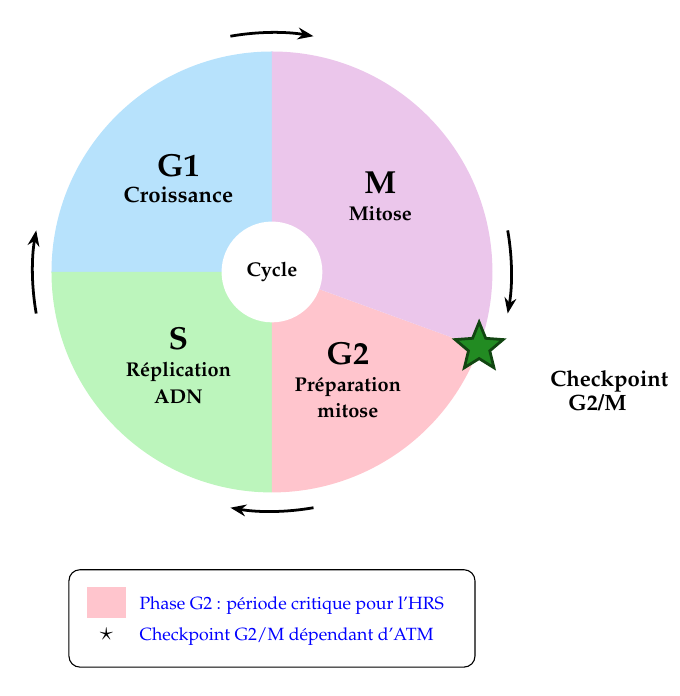
\begin{tikzpicture}[scale=0.8, transform shape]
    % Cercle du cycle cellulaire
    \def\radius{3.5}
    
    % Phase G1
    \fill[g1color!60] (0,0) -- (90:\radius) arc (90:180:\radius) -- cycle;
		\node[text width=2.5cm, align=center] at (135:2.1) {\Large\bfseries G1\\\normalsize Croissance};
    
    % Phase 
		% Phase S
		\fill[scolor!60] (0,0) -- (180:\radius) arc (180:270:\radius) -- cycle;
		\node[text width=2.5cm, align=center] at (225:2.1) {\Large\bfseries S\\\small Réplication ADN};

    % Phase G2
		\fill[g2color!80] (0,0) -- (270:\radius) arc (270:340:\radius) -- cycle;
		\node[text width=2.5cm, align=center] at (305:2.1) {\Large\bfseries G2\\\small Préparation mitose};

		% Phase M
		\fill[mcolor!60] (0,0) -- (340:\radius) arc (340:360:\radius) -- cycle;
		\fill[mcolor!60] (0,0) -- (0:\radius) arc (0:90:\radius) -- cycle;
		\node[text width=2.5cm, align=center] at (35:2.1) {\Large\bfseries M\\\small Mitose};
    
    % Cercle central
    \fill[white] (0,0) circle (0.8);
    \node[font=\small\bfseries] at (0,0) {Cycle};
    
    % Flèches de direction
    \draw[-{Stealth[length=2mm]}, line width=1pt] (100:\radius+0.3) arc (100:80:\radius+0.3);
    \draw[-{Stealth[length=2mm]}, line width=1pt] (190:\radius+0.3) arc (190:170:\radius+0.3);
    \draw[-{Stealth[length=2mm]}, line width=1pt] (280:\radius+0.3) arc (280:260:\radius+0.3);
    \draw[-{Stealth[length=2mm]}, line width=1pt] (10:\radius+0.3) arc (10:-10:\radius+0.3);
    
    % Checkpoint G2/M (étoile)
    \node[star, star points=5, star point ratio=2.25, fill=checkcolor, minimum size=0.8cm, draw=checkcolor!50!black, line width=1pt] at (340:3.5) {};
    \node[font=\tiny\bfseries, text width=1.5cm, align=center] at (340:5.5) {\normalsize Checkpoint G2/M};
    
    
    % Légende
    \node[draw, rectangle, rounded corners, fill=white, inner sep=8pt, font=\large] at (0,-5.5) {
        \begin{tabular}{cl}
        \cellcolor{g2color!80} &\footnotesize  \color{blue} Phase G2 : période critique pour l'HRS\color{black}\\
        $\star$ &\footnotesize \color{blue}Checkpoint G2/M dépendant d'ATM\color{black}
        \end{tabular}
    };
\end{tikzpicture}
\captionsetup{labelformat=empty}
\caption{\footnotesize Le cycle cellulaire avec ses quatre phases.}
\end{figure}

%==============================================================================
\normalsize 
\subsectionbox{Détection des dommages par ATM}
\footnotesize 
%==============================================================================

\noindent Le checkpoint $\bm{G2/M}$ peut être comparé à un \color{blue}\textbf{contrôle qualité}\color{black} \; avant la division cellulaire. Son rôle est de vérifier que l'ADN est intact avant d'autoriser la cellule à entrer en mitose.
\newpage
\begin{figure}[h!]
\centering
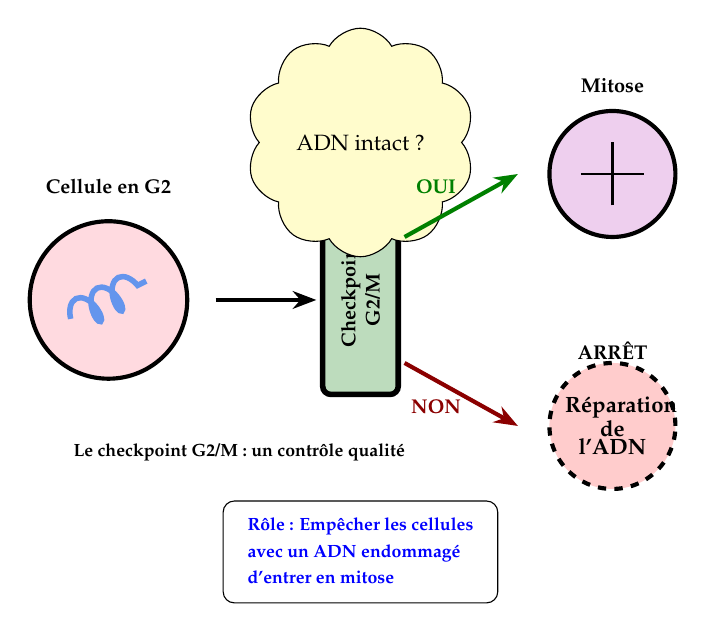
\begin{tikzpicture}[scale=0.8, transform shape]
    % Titre
    \node[font=\large\bfseries] at (0,1,5) {\footnotesize Le checkpoint G2/M : un contrôle qualité};
    
    % Cellule avant checkpoint
    \node[draw, circle, minimum size=2.5cm, fill=g2color!50, line width=1.5pt] (cell1) at (-4,1.5) {};
    \node[font=\small\bfseries] at (-4,3.3) {Cellule en G2};
    
    % ADN dans la cellule (représentation simplifiée)
    \draw[dnacolor, line width=2pt, decorate, decoration={coil, segment length=3mm, amplitude=2mm}] (-4.6,1.2) -- (-3.4,1.8);
    
    % Flèche vers checkpoint
    \draw[-{Stealth[length=3mm]}, line width=1.5pt] (-2.3,1.5) -- (-0.7,1.5);
    
    % Checkpoint (barrière)
    \node[draw, rectangle, minimum width=1.2cm, minimum height=3cm, fill=checkcolor!30, line width=2pt, rounded corners=3pt] (check) at (0,1.5) {};
    \node[font=\small\bfseries, text width=1.5cm, align=center, rotate=90] at (0,1.5) {Checkpoint G2/M};
    
    % Questions du checkpoint
    \node[draw, cloud, cloud puffs=10, cloud puff arc=120, minimum width=3cm, minimum height=1.5cm, fill=yellow!20] at (0,4) {ADN intact ?};
    
    % Deux voies possibles
    % Voie OUI (haut)
    \draw[-{Stealth[length=3mm]}, line width=1.5pt, survivecolor] (0.7,2.5) -- (2.5,3.5);
    \node[font=\small\bfseries, survivecolor] at (1.2,3.3) {OUI};
    
    % Cellule en mitose
    \node[draw, circle, minimum size=2cm, fill=mcolor!50, line width=1.5pt] (cell2) at (4,3.5) {};
    \node[font=\small\bfseries] at (4,4.9) {Mitose};
    \draw[line width=1pt] (3.5,3.5) -- (4.5,3.5);
    \draw[line width=1pt] (4,3) -- (4,4);
    
    % Voie NON (bas)
    \draw[-{Stealth[length=3mm]}, line width=1.5pt, deathcolor] (0.7,0.5) -- (2.5,-0.5);
    \node[font=\small\bfseries, deathcolor] at (1.2,-0.2) {NON};
    
    % Cellule arrêtée
    \node[draw, circle, minimum size=2cm, fill=red!20, line width=1.5pt, dashed] (cell3) at (4,-0.5) {};
    \node[font=\small\bfseries] at (4,0.7) {ARRÊT};
    \node[font=\tiny, text width=1.5cm, align=center] at (4,-0.5) {\normalsize \textbf{Réparation de l'ADN}};
    
    % Légende
    \node[draw, rectangle, fill=white, rounded corners, inner sep=5pt] at (0,-2.5) {
        \begin{tabular}{l}
        \footnotesize \color{blue}\textbf{Rôle : Empêcher les cellules}\color{black}\\
        \footnotesize \color{blue}\textbf{avec un ADN endommagé}\color{black}\\
        \footnotesize \color{blue}\textbf{d'entrer en mitose}\color{black}
        \end{tabular}
    };
\end{tikzpicture}
\captionsetup{labelformat=empty}
\caption{\footnotesize Le checkpoint $\bm{G2/M}$ agit comme un contrôle qualité vérifiant l'intégrité de l'ADN avant la division cellulaire.}
\end{figure}

\noindent Lorsqu'une cellule en phase $\bm{G2}$ reçoit des radiations ionisantes, des cassures double-brin (DSB) apparaissent dans l'ADN. La protéine $\bm{ATM}$ agit comme un \color{blue}\textbf{détecteur}\color{black} : \color{blue}\textbf{elle reconnaît ces cassures et s'active par autophosphorylation.}\color{black}

\begin{tcolorbox}[colback=blue!5, colframe=atmcolor, title=\textbf{Détection des cassures double-brin par ATM}]

\centering
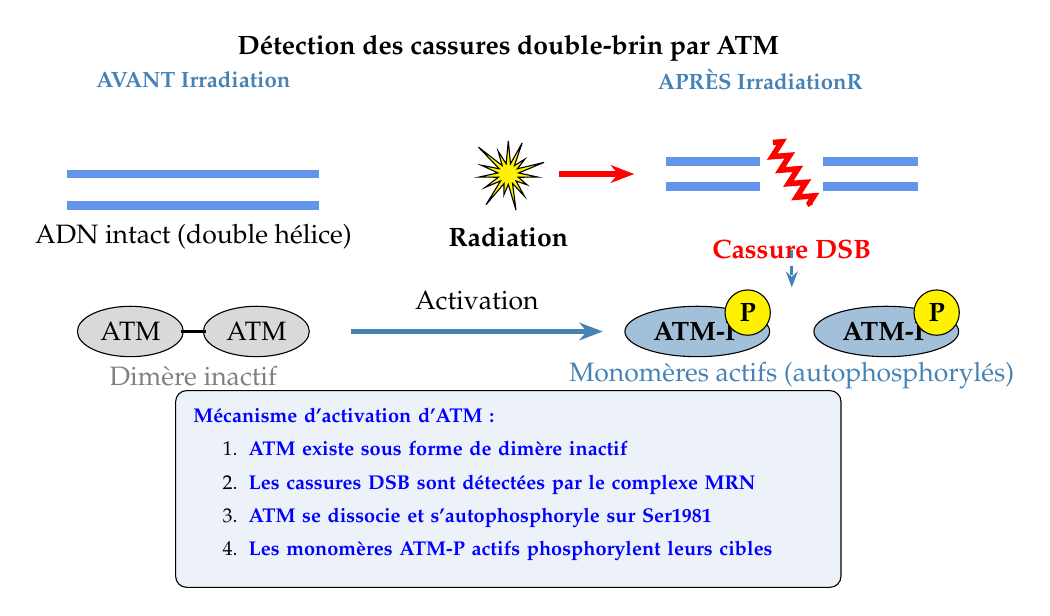
\begin{tikzpicture}[scale=0.8, transform shape]
    % Titre
    \node[font=\large\bfseries] at (0,6) {Détection des cassures double-brin par ATM};
    
    % === AVANT IRRADIATION ===
    \node[font=\bfseries, atmcolor] at (-5,5.5) {AVANT Irradiation};
    
    % ADN intact
    \draw[dnacolor, line width=3pt] (-7,4) -- (-3,4);
    \draw[dnacolor, line width=3pt] (-7,3.5) -- (-3,3.5);
    \node[font=\large] at (-5,3) {ADN intact (double hélice)};
    
    % ATM inactive (dimère)
    \node[draw, ellipse, minimum width=1.5cm, minimum height=0.8cm, fill=gray!30, font=\large] at (-6,1.5) {ATM};
    \node[draw, ellipse, minimum width=1.5cm, minimum height=0.8cm, fill=gray!30, font=\large] at (-4,1.5) {ATM};
    \draw[line width=1pt] (-5.2,1.5) -- (-4.8,1.5);
    \node[font=\large, gray] at (-5,0.8) {Dimère inactif};
    
    % === APRÈS IRRADIATION ===
    \node[font=\bfseries, atmcolor] at (4,5.5) {APRÈS IrradiationR};
    
    % Radiation
    \node[draw, starburst, starburst points=15, fill=yellow, minimum size=1.2cm] at (0,4) {};
    \node[font=\large\bfseries] at (0,3) {Radiation};
    \draw[-{Stealth[length=3mm]}, line width=2pt, red] (0.8,4) -- (2,4);
    
    % ADN avec cassure
    \draw[dnacolor, line width=3pt] (2.5,4.2) -- (4,4.2);
    \draw[dnacolor, line width=3pt] (5,4.2) -- (6.5,4.2);
    \draw[dnacolor, line width=3pt] (2.5,3.8) -- (4,3.8);
    \draw[dnacolor, line width=3pt] (5,3.8) -- (6.5,3.8);
    
    % Cassure (DSB)
    \draw[red, line width=2pt, decorate, decoration={zigzag, segment length=2mm, amplitude=1mm}] (4.2,4.5) -- (4.8,3.5);
    \node[font=\large\bfseries, red] at (4.5,2.8) {Cassure DSB};
    
    % ATM activée (monomères)
    \node[draw, ellipse, minimum width=1.5cm, minimum height=0.8cm, fill=atmcolor!50, font=\large\bfseries] at (3,1.5) {ATM-P};
    \node[draw, ellipse, minimum width=1.5cm, minimum height=0.8cm, fill=atmcolor!50, font=\large\bfseries] at (6,1.5) {ATM-P};
    
    % Phosphorylation
    \node[draw, circle, fill=yellow, minimum size=0.4cm, font=\large\bfseries] at (3.8,1.8) {P};
    \node[draw, circle, fill=yellow, minimum size=0.4cm, font=\large\bfseries] at (6.8,1.8) {P};
    
    \node[font=\large, atmcolor] at (4.5,0.8) {Monomères actifs (autophosphorylés)};
    
    % Flèche de détection
    \draw[-{Stealth[length=2mm]}, line width=1pt, dashed, atmcolor] (4.5,2.8) -- (4.5,2.2);
    
    % Flèche de transformation
    \draw[-{Stealth[length=3mm]}, line width=2pt, atmcolor] (-2.5,1.5) -- (1.5,1.5);
    \node[font=\large, rotate=0] at (-0.5,2) {Activation};
    
    % Encadré explicatif
    \node[draw, rectangle, rounded corners, fill=atmcolor!10, inner sep=8pt, text width=10cm, font=\small] at (0,-1) {
        \color{blue}\textbf{Mécanisme d'activation d'ATM :}\color{black}
        \begin{enumerate}
            \item \color{blue}\textbf{ATM existe sous forme de dimère inactif}\color{black}
            \item \color{blue}\textbf{Les cassures DSB sont détectées par le complexe MRN}\color{black}
            \item \color{blue}\textbf{ATM se dissocie et s'autophosphoryle sur Ser1981}\color{black}
            \item \color{blue}\textbf{Les monomères ATM-P actifs phosphorylent leurs cibles}\color{black}
        \end{enumerate}
    };
\end{tikzpicture}\newline
\noindent Mécanisme de détection des cassures double-brin de l'ADN par la protéine $\bm{ATM}$. L'autophosphorylation d'$\bm{ATM}$ sur la $\bm{sérine 1981}$ marque son activation.
\end{tcolorbox}



\noindent \textbf{ATM} (\textit{Ataxia Telangiectasia Mutated}) est une protéine kinase clé dans la réponse aux dommages de l'ADN. Elle agit comme un \color{blue}\textbf{détecteur}\color{black} \; des cassures double-brin (DSB), les dommages les plus dangereux pour la cellule.

\begin{tcolorbox}[colback=blue!5, colframe=atmcolor, title=\textbf{Autophosphorylation}]
 Processus par lequel une protéine ajoute un groupe phosphate ($\bm{PO4^{3-}}$) sur \textbf{elle-même}, modifiant ainsi son activité.
\noindent \textbf{Structure d'ATM : Forme inactive vs active}
\begin{center}
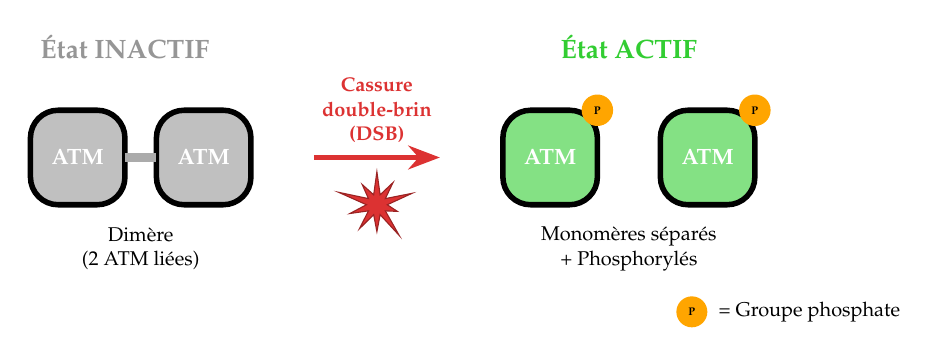
\begin{tikzpicture}[scale=0.8, transform shape]
    
    % === FORME INACTIVE (DIMÈRE) ===
    \node[font=\large\bfseries, color=atminactive] at (-4, 3) {État INACTIF};
    
    % Deux ATM liées (dimère)
    \draw[fill=atminactive!60, rounded corners=10pt, line width=2pt] (-5.5, 0.5) rectangle (-4, 2);
    \node[font=\bfseries, white] at (-4.75, 1.25) {ATM};
    
    \draw[fill=atminactive!60, rounded corners=10pt, line width=2pt] (-3.5, 0.5) rectangle (-2, 2);
    \node[font=\bfseries, white] at (-2.75, 1.25) {ATM};
    
    % Liaison entre les deux
    \draw[line width=3pt, atminactive!80] (-4, 1.25) -- (-3.5, 1.25);
    
    % Label dimère
    \node[font=\small, align=center] at (-3.75, -0.2) {Dimère\\(2 ATM liées)};
    
    % === FLÈCHE DE TRANSITION ===
    \draw[-{Stealth[length=4mm, width=3mm]}, line width=2pt, dsbcolor] (-1, 1.25) -- (1, 1.25);
    \node[font=\small\bfseries, dsbcolor, align=center] at (0, 2) {Cassure\\double-brin\\(DSB)};
    
    % Symbole DSB
    \node[starburst, starburst points=10, fill=dsbcolor, minimum size=0.8cm, draw=dsbcolor!70!black] at (0, 0.5) {};
    
    % === FORME ACTIVE (MONOMÈRES) ===
    \node[font=\large\bfseries, color=atmactive] at (4, 3) {État ACTIF};
    
    % Premier monomère avec phosphate
    \draw[fill=atmactive!60, rounded corners=10pt, line width=2pt] (2, 0.5) rectangle (3.5, 2);
    \node[font=\bfseries, white] at (2.75, 1.25) {ATM};
    \node[circle, fill=phosphocolor, minimum size=0.5cm, font=\tiny\bfseries] at (3.5, 2) {P};
    
    % Deuxième monomère avec phosphate
    \draw[fill=atmactive!60, rounded corners=10pt, line width=2pt] (4.5, 0.5) rectangle (6, 2);
    \node[font=\bfseries, white] at (5.25, 1.25) {ATM};
    \node[circle, fill=phosphocolor, minimum size=0.5cm, font=\tiny\bfseries] at (6, 2) {P};
    
    % Label monomères
    \node[font=\small, align=center] at (4, -0.2) {Monomères séparés\\+ Phosphorylés};
    
    % Légende phosphate
    \node[circle, fill=phosphocolor, minimum size=0.4cm, font=\tiny\bfseries] at (5, -1.2) {P};
    \node[font=\small, right] at (5.3, -1.2) {= Groupe phosphate};
    
\end{tikzpicture}\newline
\end{center}
\noindent {\textbf{Activation d'ATM par autophosphorylation.} À l'état normal, ATM existe sous forme de dimère inactif. La détection d'une cassure double-brin (DSB) provoque la séparation du dimère et l'autophosphorylation des monomères, les rendant actifs.}
\end{tcolorbox}


\begin{tcolorbox}[colback=blue!5, colframe=atmcolor, title=\textbf{Mécanisme d'activation en 3 étapes}]
\begin{center}
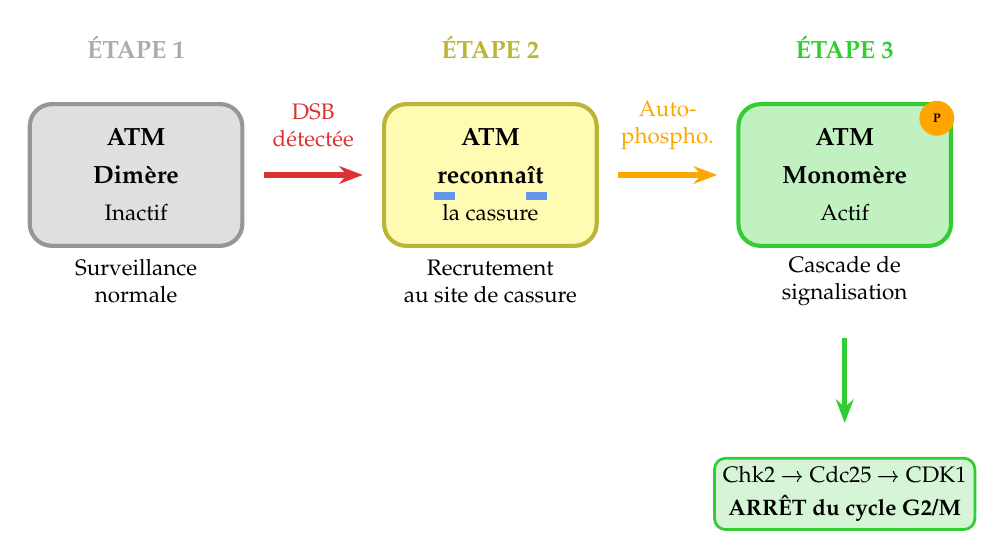
\begin{tikzpicture}[scale=0.9, transform shape,
    box/.style={rectangle, rounded corners=8pt, minimum width=3cm, minimum height=2cm, line width=1.5pt, align=center},
    arrow/.style={-{Stealth[length=3mm]}, line width=2pt}
]
    
    % === ÉTAPE 1 : État normal ===
    \node[box, fill=atminactive!30, draw=atminactive] (step1) at (0, 0) {
        \textbf{ATM}\\[3pt]
        \textbf{Dimère}\\[3pt]
        \small Inactif
    };
    \node[font=\bfseries, atminactive!80] at (0, 1.8) {ÉTAPE 1};
    \node[font=\small, align=center] at (0, -1.5) {Surveillance\\normale};
    
    % === FLÈCHE 1→2 ===
    \draw[arrow, dsbcolor] (1.8, 0) -- (3.2, 0);
    \node[font=\small, dsbcolor, align=center] at (2.5, 0.7) {DSB\\détectée};
    
    % === ÉTAPE 2 : Détection ===
    \node[box, fill=yellow!30, draw=yellow!70!black] (step2) at (5, 0) {
        \textbf{ATM}\\[3pt]
        \textbf{reconnaît}\\[3pt]
        \small la cassure
    };
    \node[font=\bfseries, yellow!70!black] at (5, 1.8) {ÉTAPE 2};
    \node[font=\small, align=center] at (5, -1.5) {Recrutement\\au site de cassure};
    
    % Symbole ADN cassé
    \draw[dnacolor, line width=3pt] (4.2, -0.3) -- (4.5, -0.3);
    \draw[dnacolor, line width=3pt] (5.5, -0.3) -- (5.8, -0.3);
    \node[font=\tiny, dsbcolor] at (5, -0.3) {};
    
    % === FLÈCHE 2→3 ===
    \draw[arrow, phosphocolor] (6.8, 0) -- (8.2, 0);
    \node[font=\small, phosphocolor, align=center] at (7.5, 0.7) {Auto-\\phospho.};
    
    % === ÉTAPE 3 : Activation ===
    \node[box, fill=atmactive!30, draw=atmactive] (step3) at (10, 0) {
        \textbf{ATM}\\[3pt]
        \textbf{Monomère}\\[3pt]
        \small Actif
    };
    \node[circle, fill=phosphocolor, minimum size=0.4cm, font=\tiny\bfseries] at (11.3, 0.8) {P};
    \node[font=\bfseries, atmactive] at (10, 1.8) {ÉTAPE 3};
    \node[font=\small, align=center] at (10, -1.5) {Cascade de\\signalisation};
    
    % === FLÈCHE VERS CASCADE ===
    \draw[arrow, atmactive] (10, -2.3) -- (10, -3.5);
    
    % === CASCADE ===
    \node[rectangle, rounded corners, fill=atmactive!20, draw=atmactive, line width=1pt, align=center, font=\small] at (10, -4.5) {
        Chk2 → Cdc25 → CDK1\\[2pt]
        \textbf{ARRÊT du cycle G2/M}
    };
    
\end{tikzpicture}\newline
\end{center}
\noindent {\textbf{Les 3 étapes de l'activation d'ATM.} (1) ATM surveille l'ADN sous forme inactive. (2) Détection et recrutement au site de cassure. (3) Autophosphorylation et activation de la cascade de signalisation menant à l'arrêt du cycle cellulaire.}\par
\end{tcolorbox}

%==============================================================================
\normalsize 
\subsectionbox{La cascade de signalisation}
\footnotesize 
%==============================================================================

\noindent Une fois activée, $\bm{ATM}$ déclenche une cascade de phosphorylations qui aboutit au blocage du complexe $\bm{CDK1}$/$\bm{Cycline B}$, le "moteur" de l'entrée en mitose.\par

\begin{tcolorbox}[colback=blue!5, colframe=atmcolor, title=\textbf{La cascade de signalisation}]
\begin{center}
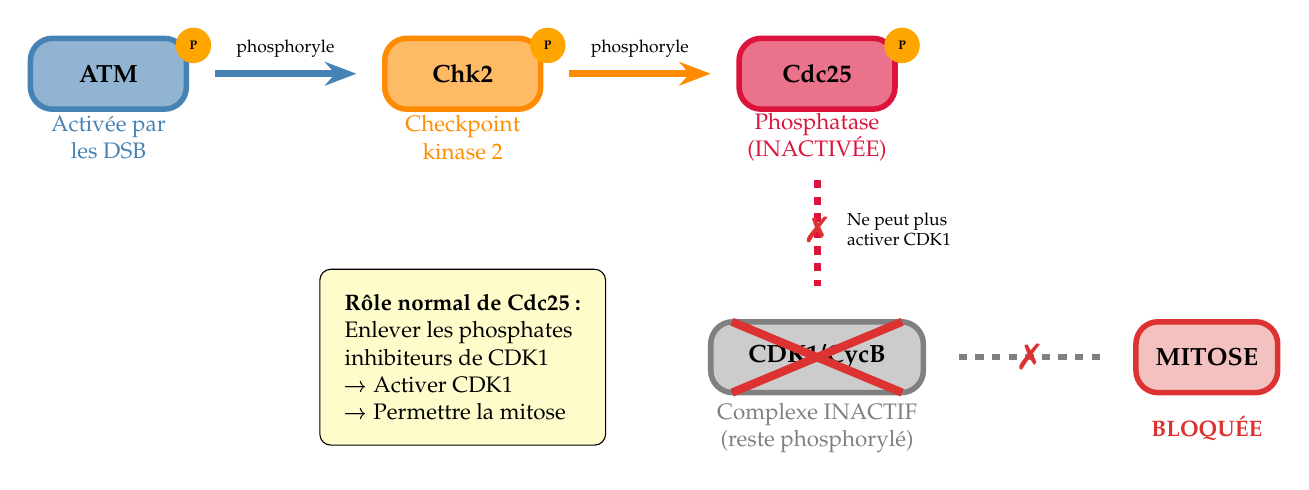
\begin{tikzpicture}[
    scale=0.9, 
    transform shape,
    protein/.style={rectangle, rounded corners=8pt, minimum width=2.2cm, minimum height=1cm, line width=2pt, font=\bfseries, align=center},
    arrow/.style={-{Stealth[length=4mm, width=3mm]}, line width=2.5pt},
    phospho/.style={circle, fill=phosphocolor, minimum size=0.5cm, font=\tiny\bfseries}
]
    
    % === ATM ===
    \node[protein, fill=atmcolor!60, draw=atmcolor] (atm) at (0, 0) {ATM};
    \node[phospho] at (1.2, 0.4) {P};
    \node[font=\small, atmcolor, align=center] at (0, -0.9) {Activée par\\les DSB};
    
    % Flèche ATM → Chk2
    \draw[arrow, atmcolor] (1.5, 0) -- (3.5, 0);
    \node[font=\scriptsize, above] at (2.5, 0.1) {phosphoryle};
    
    % === Chk2 ===
    \node[protein, fill=chk2color!60, draw=chk2color] (chk2) at (5, 0) {Chk2};
    \node[phospho] at (6.2, 0.4) {P};
    \node[font=\small, chk2color, align=center] at (5, -0.9) {Checkpoint\\kinase 2};
    
    % Flèche Chk2 → Cdc25
    \draw[arrow, chk2color] (6.5, 0) -- (8.5, 0);
    \node[font=\scriptsize, above] at (7.5, 0.1) {phosphoryle};
    
    % === Cdc25 ===
    \node[protein, fill=cdc25color!60, draw=cdc25color] (cdc25) at (10, 0) {Cdc25};
    \node[phospho] at (11.2, 0.4) {P};
    \node[font=\small, cdc25color, align=center] at (10, -0.9) {Phosphatase\\(INACTIVÉE)};
    
    % Flèche Cdc25 --X--> CDK1
    \draw[line width=2.5pt, cdc25color, dashed] (10, -1.5) -- (10, -3);
    \node[font=\Large, stopcolor] at (10, -2.2) {\ding{55}};
    \node[font=\scriptsize, right, align=left] at (10.3, -2.2) {Ne peut plus\\activer CDK1};
    
    % === CDK1/CycB (bloqué) ===
    \node[protein, fill=gray!40, draw=gray, minimum width=3cm] (cdk1) at (10, -4) {CDK1/CycB};
    \node[font=\small, gray, align=center] at (10, -5) {Complexe INACTIF\\(reste phosphorylé)};
    
    % Croix sur CDK1
    \draw[stopcolor, line width=3pt] (8.8, -3.5) -- (11.2, -4.5);
    \draw[stopcolor, line width=3pt] (8.8, -4.5) -- (11.2, -3.5);
    
    % === Flèche vers MITOSE bloquée ===
    \draw[line width=2pt, gray, dashed] (12, -4) -- (14, -4);
    \node[font=\Large, stopcolor] at (13, -4) {\ding{55}};
    
    % === MITOSE ===
    \node[protein, fill=stopcolor!30, draw=stopcolor, minimum width=2cm] (mitose) at (15.5, -4) {MITOSE};
    \node[font=\small\bfseries, stopcolor] at (15.5, -5) {BLOQUÉE};
    
    % === Encadré explicatif ===
    \node[draw, rectangle, rounded corners, fill=yellow!20, inner sep=10pt, font=\small, align=left] at (5, -4) {
        \textbf{Rôle normal de Cdc25 :}\\
        Enlever les phosphates\\
        inhibiteurs de CDK1\\
        → Activer CDK1\\
        → Permettre la mitose
    };
    
\end{tikzpicture}\newline
\end{center}
\noindent \textbf{La cascade ATM $\rightarrow$ Chk2 $\rightarrow$ Cdc25 $\dashv$ CDK1.} ATM activée phosphoryle Chk2, qui phosphoryle Cdc25. Cdc25 phosphorylée est inactive et ne peut plus activer CDK1/Cycline B. Sans CDK1 actif, la cellule ne peut pas entrer en mitose.
\end{tcolorbox}


\begin{tcolorbox}[colback=blue!5, colframe=atmcolor, title=\textbf{CDK1/Cycline B : Le moteur de la mitose}]
\begin{center}
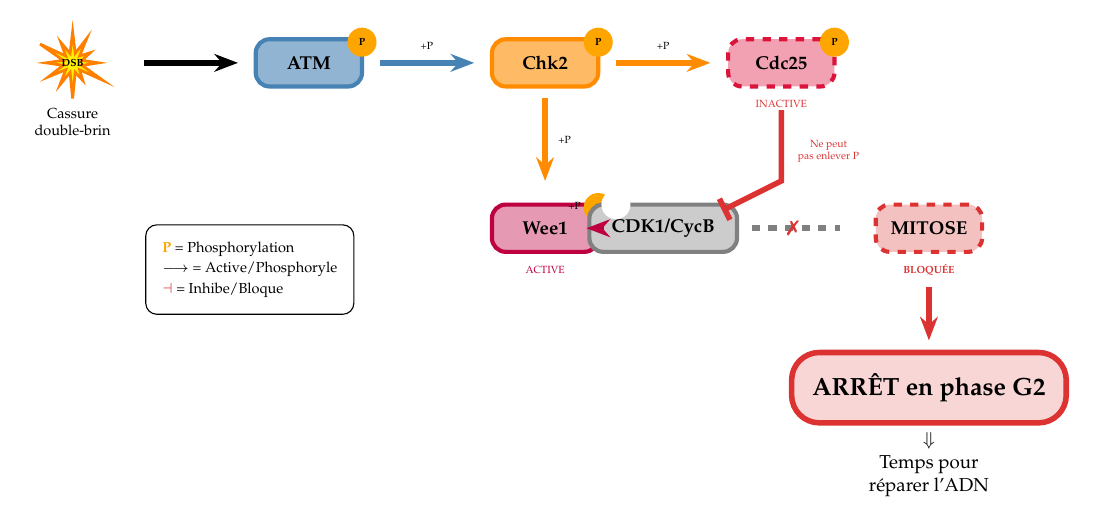
\begin{tikzpicture}[
    scale=0.75, 
    transform shape,
    box/.style={rectangle, rounded corners=5pt, minimum width=1.8cm, minimum height=0.8cm, line width=1.5pt, font=\small\bfseries, align=center},
    arrow/.style={-{Stealth[length=3mm]}, line width=2pt},
    inhibit/.style={-{Bar[width=3mm]}, line width=2pt, stopcolor}
]
    
    % === Dommage ADN ===
    \node[starburst, starburst points=12, fill=yellow, minimum size=1.2cm, draw=orange, line width=1pt] (dsb) at (0, 0) {};
    \node[font=\tiny\bfseries] at (0, 0) {DSB};
    \node[font=\scriptsize, align=center] at (0, -1) {Cassure\\double-brin};
    
    % Flèche vers ATM
    \draw[arrow, black] (1.2, 0) -- (2.8, 0);
    
    % === ATM ===
    \node[box, fill=atmcolor!60, draw=atmcolor] (atm) at (4, 0) {ATM};
    \node[circle, fill=phosphocolor, minimum size=0.35cm, font=\tiny\bfseries] at (4.9, 0.35) {P};
    
    % Flèche ATM vers Chk2
    \draw[arrow, atmcolor] (5.2, 0) -- (6.8, 0);
    \node[font=\tiny, above] at (6, 0.1) {+P};
    
    % === Chk2 ===
    \node[box, fill=chk2color!60, draw=chk2color] (chk2) at (8, 0) {Chk2};
    \node[circle, fill=phosphocolor, minimum size=0.35cm, font=\tiny\bfseries] at (8.9, 0.35) {P};
    
    % Flèche Chk2 vers Cdc25
    \draw[arrow, chk2color] (9.2, 0) -- (10.8, 0);
    \node[font=\tiny, above] at (10, 0.1) {+P};
    
    % === Cdc25 (inactivée) ===
    \node[box, fill=cdc25color!40, draw=cdc25color, dashed] (cdc25) at (12, 0) {Cdc25};
    \node[circle, fill=phosphocolor, minimum size=0.35cm, font=\tiny\bfseries] at (12.9, 0.35) {P};
    \node[font=\tiny, stopcolor] at (12, -0.7) {INACTIVE};
    
    % Inhibition de Wee1 par Chk2
    \draw[arrow, chk2color] (8, -0.6) -- (8, -2);
    \node[font=\tiny, right] at (8.1, -1.3) {+P};
    
    % === Wee1 (activée) ===
    \node[box, fill=purple!40, draw=purple] (wee1) at (8, -2.8) {Wee1};
    \node[circle, fill=phosphocolor, minimum size=0.35cm, font=\tiny\bfseries] at (8.9, -2.45) {P};
    \node[font=\tiny, purple] at (8, -3.5) {ACTIVE};
    
    % === CDK1/CycB ===
    \node[box, fill=gray!40, draw=gray, minimum width=2.5cm] (cdk1) at (10, -2.8) {CDK1/CycB};
    
    % Flèche Wee1 ajoute P sur CDK1
    \draw[arrow, purple] (9, -2.8) -- (8.7, -2.8);
    \node[circle, fill=stopcolor, minimum size=0.3cm, font=\tiny\bfseries, white] at (9.2, -2.4) {P};
    \node[font=\tiny, above] at (8.5, -2.6) {+P};
    
    % Cdc25 ne peut pas enlever P
    \draw[inhibit] (12, -0.8) -- (12, -2) -- (11, -2.5);
    \node[font=\tiny, stopcolor, align=center] at (12.8, -1.5) {Ne peut\\pas enlever P};
    
    % Flèche vers mitose bloquée
    \draw[line width=2pt, gray, dashed] (11.5, -2.8) -- (13, -2.8);
    \node[font=\normalsize, stopcolor] at (12.2, -2.8) {\ding{55}};
    
    % === Mitose ===
    \node[box, fill=stopcolor!30, draw=stopcolor, dashed] (mitose) at (14.5, -2.8) {MITOSE};
    \node[font=\tiny\bfseries, stopcolor] at (14.5, -3.5) {BLOQUÉE};
    
    % === Légende ===
    \node[draw, rectangle, rounded corners, fill=white, inner sep=8pt, font=\scriptsize, align=left] at (3, -3.5) {
        \textcolor{phosphocolor}{\textbf{P}} = Phosphorylation\\[2pt]
        $\longrightarrow$ = Active/Phosphoryle\\[2pt]
        \textcolor{stopcolor}{$\dashv$} = Inhibe/Bloque
    };
    
    % === ARRÊT G2 ===
    \node[draw, rectangle, rounded corners=10pt, fill=stopcolor!20, line width=2pt, draw=stopcolor, inner sep=10pt] at (14.5, -5.5) {
        \textbf{\large ARRÊT en phase G2}
    };
    \draw[arrow, stopcolor] (14.5, -3.8) -- (14.5, -4.7);
    
    % Temps pour réparation
    \node[font=\small, align=center] at (14.5, -6.8) {$\Downarrow$\\Temps pour\\réparer l'ADN};
    
\end{tikzpicture}\newline
\end{center}
\noindent \textbf{Cascade complète de signalisation ATM.} Les DSB activent ATM, qui phosphoryle Chk2. Chk2 a deux effets : (1) il inactive Cdc25 (qui ne peut plus activer CDK1), et (2) il active Wee1 (qui maintient CDK1 inactif en le phosphorylant). Résultat : CDK1/Cycline B reste inactif et la mitose est bloquée.
\end{tcolorbox}










\vspace{0.5cm}

\begin{center}
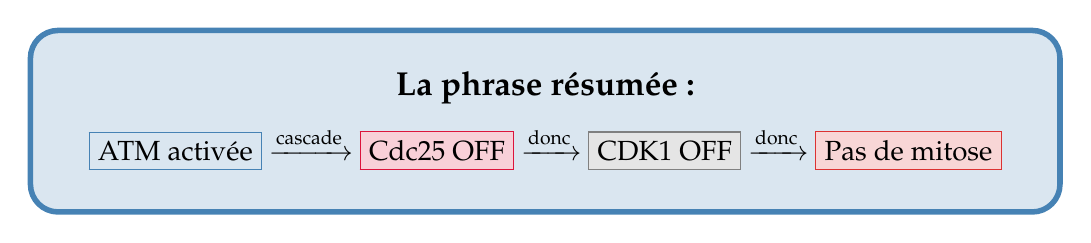
\begin{tikzpicture}
    \node[rectangle, rounded corners=10pt, fill=atmcolor!20, draw=atmcolor, line width=2pt, inner sep=15pt] {
        \begin{tabular}{c}
        \textbf{\large La phrase résumée :}\\[8pt]
        \fcolorbox{atmcolor}{atmcolor!20}{ATM activée} 
        $\xrightarrow{\text{cascade}}$ 
        \fcolorbox{cdc25color}{cdc25color!20}{Cdc25 OFF} 
        $\xrightarrow{\text{donc}}$ 
        \fcolorbox{gray}{gray!20}{CDK1 OFF} 
        $\xrightarrow{\text{donc}}$ 
        \fcolorbox{stopcolor}{stopcolor!20}{Pas de mitose}
        \end{tabular}
    };
\end{tikzpicture}
\end{center}



\begin{figure}[h!]
\centering
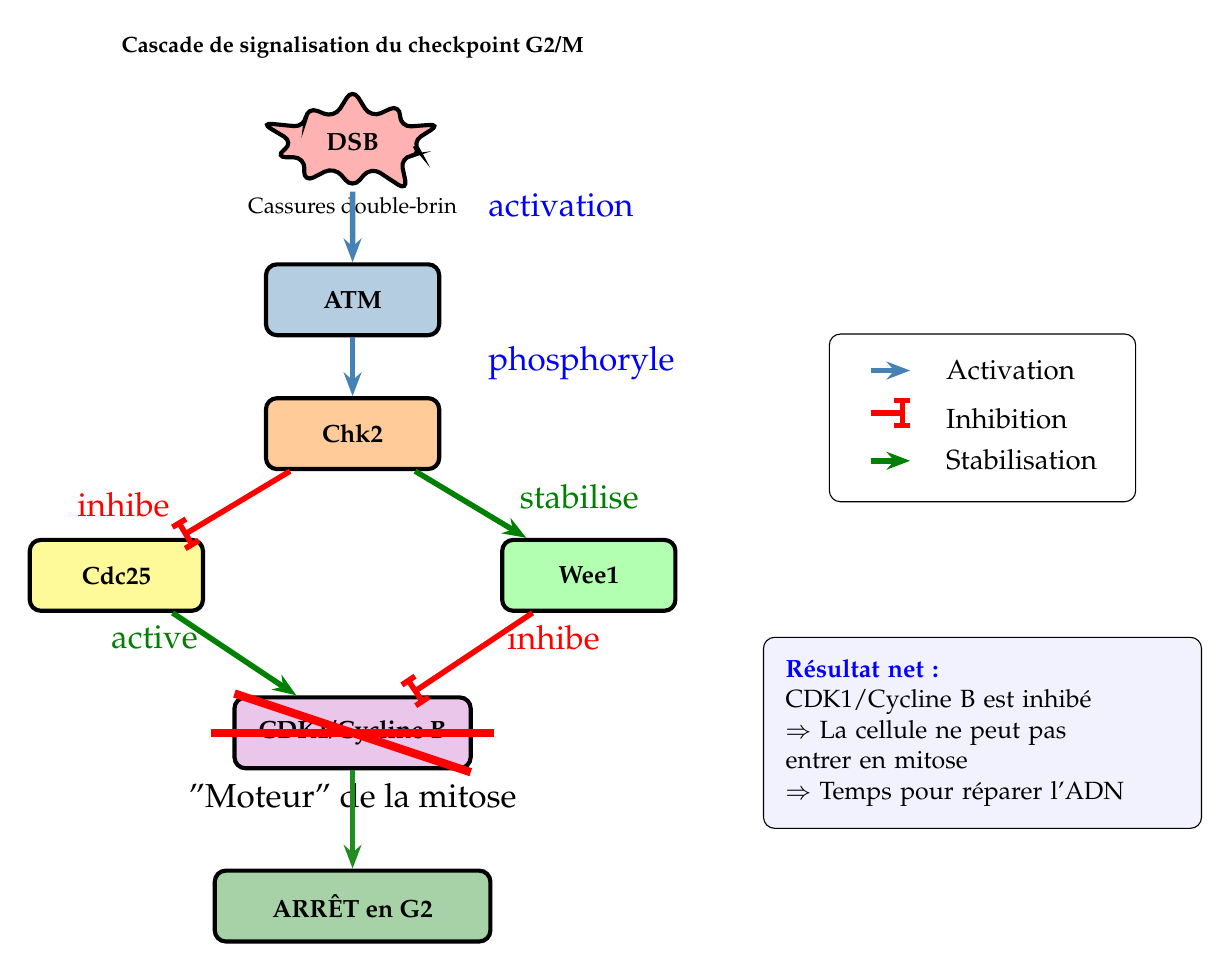
\begin{tikzpicture}[
    node distance=1.2cm,
    box/.style={draw, rectangle, rounded corners, minimum width=2.2cm, minimum height=0.9cm, font=\small\bfseries, line width=1.5pt},
    arrow/.style={-{Stealth[length=3mm]}, line width=2pt},
    inhibit/.style={-{Bar[length=2mm]}, line width=2pt, red}
]
    % Titre
    \node[font=\large\bfseries] at (0,7.7) {\footnotesize Cascade de signalisation du checkpoint G2/M};
    
    % Dommages ADN
    \node[box, fill=red!30, starburst, starburst points=10, minimum width=2.5cm] (damage) at (0,6.5) {DSB};
    \node[font=\footnotesize] at (0,5.7) {Cassures double-brin};
    
    % ATM
    \node[box, fill=atmcolor!40] (atm) at (0,4.5) {ATM};
    \draw[arrow, atmcolor] (damage) -- (atm);
    \node[font=\large, blue, right] at (1.6,5.7) {activation};
    
    % Chk2
    \node[box, fill=orange!40] (chk2) at (0,2.8) {Chk2};
    \draw[arrow, atmcolor] (atm) -- (chk2);
    \node[font=\large, blue, right] at (1.6,3.7) {phosphoryle};
    
    % Cdc25
    \node[box, fill=yellow!40] (cdc25) at (-3,1) {Cdc25};
    \draw[inhibit] (chk2) -- (cdc25);
    \node[font=\large, red, left] at (-2.2,1.9) {inhibe};
    
    % CDK1/CycB
    \node[box, fill=mcolor!60, minimum width=3cm] (cdk) at (0,-1) {CDK1/Cycline B};
    \node[font=\large] at (0,-1.8) {"Moteur" de la mitose};
    
    % Wee1
    \node[box, fill=green!30] (wee1) at (3,1) {Wee1};
    \draw[arrow, green!50!black] (chk2) -- (wee1);
    \node[font=\large, right, green!50!black] at (2,2) {stabilise};
    
    % Flèches vers CDK1
    \draw[arrow, green!50!black] (cdc25) -- node[font=\large, left, pos=0.3] {active} (cdk);
    \draw[inhibit] (wee1) -- node[font=\large, right, pos=0.3] {inhibe} (cdk);
    
    % Résultat
    \node[box, fill=checkcolor!40, minimum width=3.5cm] (arret) at (0,-3.2) {ARRÊT en G2};
    \draw[arrow, checkcolor] (cdk) -- (arret);
    
    % Cercle d'inhibition nette sur CDK1
    \draw[red, line width=3pt] (-1.8,-1) -- (1.8,-1);
    \draw[red, line width=3pt] (-1.5,-0.5) -- (1.5,-1.5);
    
    % Légende
    \node[draw, rectangle, rounded corners, fill=white, inner sep=8pt] at (8,3) {
        \begin{tabular}{cl}
        \tikz\draw[arrow, atmcolor] (0,0) -- (0.5,0); & Activation\\[3pt]
        \tikz\draw[inhibit] (0,0) -- (0.5,0); & Inhibition\\[3pt]
        \tikz\draw[arrow, green!50!black] (0,0) -- (0.5,0); & Stabilisation
        \end{tabular}
    };
    
    % Encadré résumé
    \node[draw, rectangle, rounded corners, fill=blue!5, inner sep=8pt, text width=5cm, font=\small] at (8,-1) {
        \color{blue}\textbf{Résultat net :}\color{black}\\
        CDK1/Cycline B est inhibé\\
        $\Rightarrow$ La cellule ne peut pas\\
        entrer en mitose\\
        $\Rightarrow$ Temps pour réparer l'ADN
    };
\end{tikzpicture}
\captionsetup{labelformat=empty}
\caption{\footnotesize Cascade de signalisation déclenchée par $\bm{ATM}$. La double action sur $\bm{Cdc25}$ (inhibition) et Wee1 (stabilisation) assure un blocage efficace de $\bm{CDK1}$/$\bm{Cycline B}$.}
\end{figure}

\newpage


%==============================================================================
\normalsize 
\subsectionbox{Le problème aux faibles doses : le seuil d'activation d'ATM}
\footnotesize 
%==============================================================================

\noindent Voici le point critique : \textbf{ATM a besoin d'un seuil minimum de dommages pour s'activer efficacement}. C'est ce seuil qui explique l'hyper-radiosensibilité aux faibles doses.

\begin{figure}[h!]
\centering
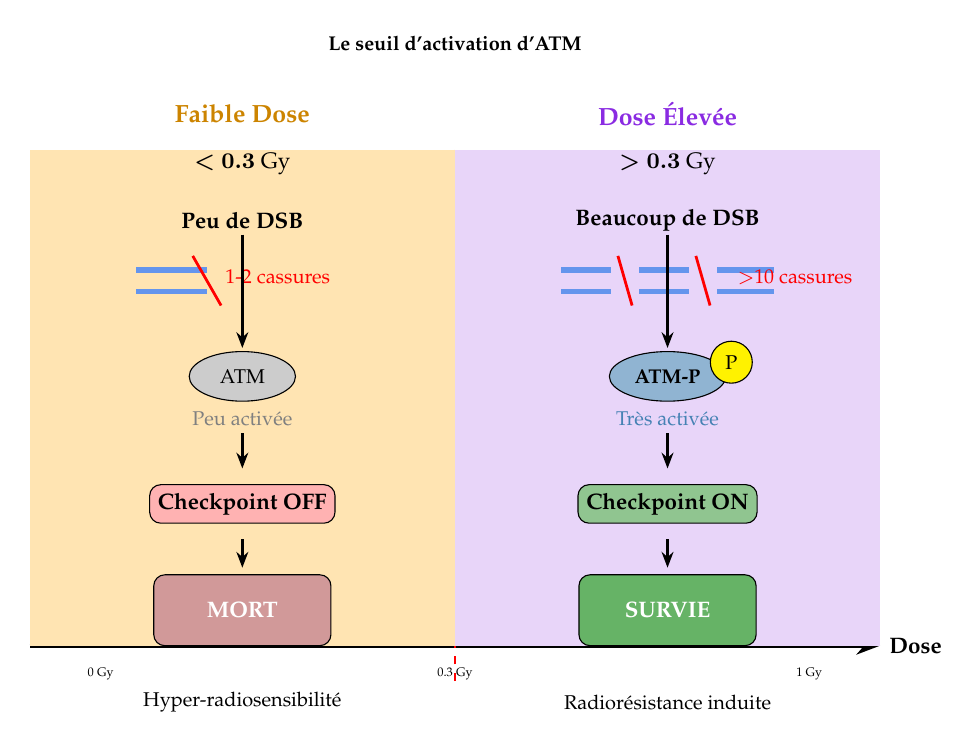
\begin{tikzpicture}[scale=0.9, transform shape]
    % Titre
    \node[font=\large\bfseries] at (0,8.5) {\footnotesize Le seuil d'activation d'ATM};
    
    % Axe des doses
    \draw[-{Stealth[length=3mm]}, line width=1.5pt] (-6,0) -- (6,0);
    \node[font=\small\bfseries] at (6.5,0) {Dose};
    \node[font=\tiny] at (-5,-0.4) {0 Gy};
    \node[font=\tiny] at (0,-0.4) {0.3 Gy};
    \node[font=\tiny] at (5,-0.4) {1 Gy};
    
    % Ligne de seuil
    \draw[dashed, line width=1pt, red] (0,-0.5) -- (0,7);
    \node[font=\small\bfseries, red, rotate=90] at (-0.5,3.5) {Seuil $D_c$};
    
    % Zone faible dose
    \fill[lowdose!30] (-6,0) rectangle (0,7);
    \node[font=\bfseries, lowdose!80!black] at (-3,7.5) {Faible Dose};
    \node[font=\small] at (-3,6.8) {$\bm{< 0.3}$ Gy};
    
    % Zone dose plus élevée
    \fill[highdose!20] (0,0) rectangle (6,7);
    \node[font=\bfseries, highdose] at (3,7.5) {Dose Élevée};
    \node[font=\small] at (3,6.8) {$\bm{> 0.3}$ Gy};
    
    % === Colonne gauche (faible dose) ===
    % Peu de DSB
    \node[font=\small\bfseries] at (-3,6) {Peu de DSB};
    \draw[dnacolor, line width=2pt] (-4.5,5.3) -- (-3.5,5.3);
    \draw[dnacolor, line width=2pt] (-4.5,5) -- (-3.5,5);
    \draw[red, line width=1pt] (-3.7,5.5) -- (-3.3,4.8);
    \node[font=\footnotesize, red] at (-2.5,5.2) {1-2 cassures};
    
    % ATM peu activée
    \node[draw, ellipse, fill=gray!40, minimum width=1.5cm, minimum height=0.7cm, font=\footnotesize] at (-3,3.8) {ATM};
    \node[font=\footnotesize, gray] at (-3,3.2) {Peu activée};
    
    % Checkpoint OFF
    \node[draw, rectangle, rounded corners, fill=red!30, minimum width=2cm, font=\small\bfseries] at (-3,2) {Checkpoint OFF};
    
    % Résultat
    \node[draw, rectangle, rounded corners, fill=deathcolor!40, minimum width=2.5cm, minimum height=1cm, font=\small\bfseries, text=white] at (-3,0.5) {MORT};
    \node[font=\footnotesize] at (-3,-0.8) {Hyper-radiosensibilité};
    
    % === Colonne droite (dose élevée) ===
    % Beaucoup de DSB
    \node[font=\small\bfseries] at (3,6) {Beaucoup de DSB};
    \draw[dnacolor, line width=2pt] (1.5,5.3) -- (2.2,5.3);
    \draw[dnacolor, line width=2pt] (2.6,5.3) -- (3.3,5.3);
    \draw[dnacolor, line width=2pt] (3.7,5.3) -- (4.5,5.3);
    \draw[dnacolor, line width=2pt] (1.5,5) -- (2.2,5);
    \draw[dnacolor, line width=2pt] (2.6,5) -- (3.3,5);
    \draw[dnacolor, line width=2pt] (3.7,5) -- (4.5,5);
    \draw[red, line width=1pt] (2.3,5.5) -- (2.5,4.8);
    \draw[red, line width=1pt] (3.4,5.5) -- (3.6,4.8);
    \node[font=\footnotesize, red] at (4.8,5.2) {$>$10 cassures};
    
    % ATM très activée
    \node[draw, ellipse, fill=atmcolor!60, minimum width=1.5cm, minimum height=0.7cm, font=\footnotesize\bfseries] at (3,3.8) {ATM-P};
    \node[draw, circle, fill=yellow, minimum size=0.3cm, font=\footnotesize] at (3.9,4) {P};
    \node[font=\footnotesize, atmcolor] at (3,3.2) {Très activée};
    
    % Checkpoint ON
    \node[draw, rectangle, rounded corners, fill=checkcolor!50, minimum width=2cm, font=\small\bfseries] at (3,2) {Checkpoint ON};
    
    % Résultat
    \node[draw, rectangle, rounded corners, fill=survivecolor!60, minimum width=2.5cm, minimum height=1cm, font=\small\bfseries, text=white] at (3,0.5) {SURVIE};
    \node[font=\footnotesize] at (3,-0.8) {Radiorésistance induite};
    
    % Flèches descendantes
    \draw[-{Stealth[length=2mm]}, line width=1pt] (-3,5.8) -- (-3,4.2);
    \draw[-{Stealth[length=2mm]}, line width=1pt] (-3,3) -- (-3,2.5);
    \draw[-{Stealth[length=2mm]}, line width=1pt] (-3,1.5) -- (-3,1.1);
    
    \draw[-{Stealth[length=2mm]}, line width=1pt] (3,5.8) -- (3,4.2);
    \draw[-{Stealth[length=2mm]}, line width=1pt] (3,3) -- (3,2.5);
    \draw[-{Stealth[length=2mm]}, line width=1pt] (3,1.5) -- (3,1.1);
\end{tikzpicture}
\captionsetup{labelformat=empty}
\caption{Comparaison de la réponse cellulaire aux faibles et fortes doses. Le seuil d'activation d'$\bm{ATM}$ ($\bm{D_c} \approx \bm{0.2}-\bm{0.5}$ Gy) détermine si le checkpoint sera activé ou non.}
\end{figure}

\begin{table}[h!]
\centering
\captionsetup{labelformat=empty}
\caption{\footnotesize Comparaison des réponses cellulaires selon la dose}
\begin{tabular}{lcc}
\toprule
\footnotesize \textbf{Paramètre}&\footnotesize \textbf{Faible dose ($\bm{< D_c}$)}&\footnotesize \textbf{Dose élevée ($\bm{> D_c}$)}\\
\midrule
\footnotesize Nombre de DSB&\footnotesize Faible (1-5)&\footnotesize Élevé ($\bm{>}$10) \\
\footnotesize Activation ATM&\footnotesize Faible/Absente&\footnotesize Forte \\
\footnotesize Checkpoint G2/M&\footnotesize Non activé&\footnotesize Activé \\
\footnotesize Devenir cellulaire&\footnotesize Mitose avec ADN cassé&\footnotesize Arrêt et réparation \\
\footnotesize \textbf{Résultat}&\footnotesize \textbf{MORT (HRS)}&\footnotesize \textbf{SURVIE (IRR)} \\
\bottomrule
\end{tabular}
\end{table}
\newpage

\begin{comment}

\end{comment}

%==============================================================================
\normalsize 
\subsectionbox{Mécanisme détaillé de l'hyper-radiosensibilité}
\footnotesize 
%==============================================================================


\begin{figure}[h!]
\centering
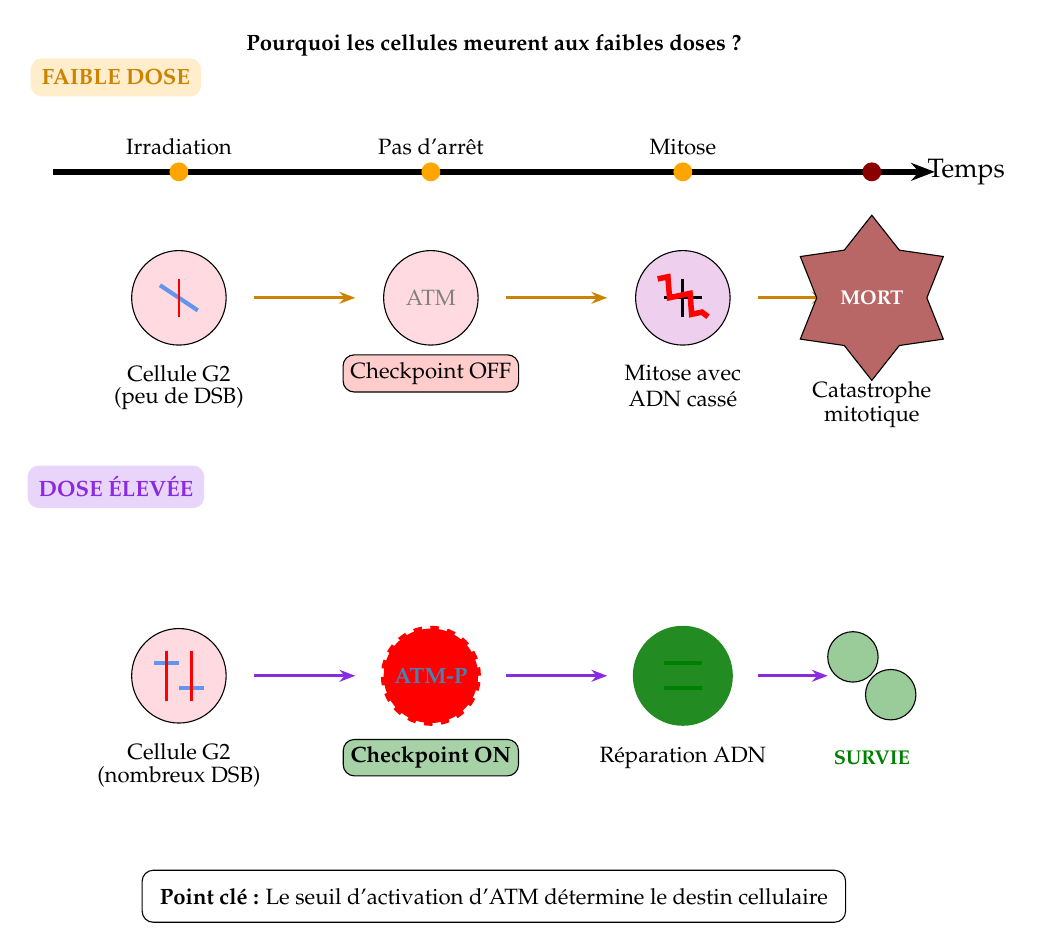
\begin{tikzpicture}[scale=0.8, transform shape]
    % Titre
    \node[font=\large\bfseries] at (0,9) {\normalsize Pourquoi les cellules meurent aux faibles doses ?};
    
    % Timeline horizontale
    \draw[-{Stealth[length=3mm]}, line width=2pt] (-7,7) -- (7,7);
    \node[font=\large] at (7.5,7) {Temps};
    
    % === FAIBLE DOSE (haut) ===
    \node[font=\bfseries, lowdose!80!black, fill=lowdose!20, rounded corners, inner sep=5pt] at (-6,8.5) {FAIBLE DOSE};
    
    % Étape 1 : Cellule G2 irradiée
    \node[draw, circle, minimum size=1.5cm, fill=g2color!50] (c1) at (-5,5) {};
    \draw[dnacolor, line width=1.5pt] (-5.3,5.2) -- (-4.7,4.8);
    \draw[red, line width=1pt] (-5,5.3) -- (-5,4.7);
    \node[font=\normalsize] at (-5,3.8) {Cellule G2};
    \node[font=\normalsize] at (-5,3.4) {(peu de DSB)};
    
    % Point sur timeline
    \fill[lowdose] (-5,7) circle (0.15);
    \node[font=\normalsize] at (-5,7.4) {Irradiation};
    
    % Flèche
    \draw[-{Stealth[length=2mm]}, line width=1pt, lowdose!80!black] (-3.8,5) -- (-2.2,5);
    
    % Étape 2 : ATM inactive, checkpoint non activé
    \node[draw, circle, minimum size=1.5cm, fill=g2color!50] (c2) at (-1,5) {};
    \node[font=\normalsize, gray] at (-1,5) {ATM};
    \node[draw, rectangle, fill=red!20, font=\normalsize, rounded corners] at (-1,3.8) {Checkpoint OFF};
    
    % Point sur timeline
    \fill[lowdose] (-1,7) circle (0.15);
    \node[font=\normalsize] at (-1,7.4) {Pas d'arrêt};
    
    % Flèche
    \draw[-{Stealth[length=2mm]}, line width=1pt, lowdose!80!black] (0.2,5) -- (1.8,5);
    
    % Étape 3 : Entrée en mitose avec ADN cassé
    \node[draw, circle, minimum size=1.5cm, fill=mcolor!50] (c3) at (3,5) {};
    \draw[line width=1pt] (2.7,5) -- (3.3,5);
    \draw[line width=1pt] (3,4.7) -- (3,5.3);
    \draw[red, line width=2pt, decorate, decoration={zigzag, amplitude=1mm}] (2.6,5.3) -- (3.4,4.7);
    \node[font=\normalsize] at (3,3.8) {Mitose avec};
    \node[font=\normalsize] at (3,3.4) {ADN cassé};
    
    % Point sur timeline
    \fill[lowdose] (3,7) circle (0.15);
    \node[font=\normalsize] at (3,7.4) {Mitose};
    
    % Flèche
    \draw[-{Stealth[length=2mm]}, line width=1pt, lowdose!80!black] (4.2,5) -- (5.3,5);
    
    % Étape 4 : Catastrophe mitotique / Mort
    \node[draw, star, star points=6, minimum size=1.8cm, fill=deathcolor!60, font=\small\bfseries, text=white] (death) at (6,5) {MORT};
    \node[font=\normalsize] at (6,3.5) {Catastrophe};
    \node[font=\normalsize] at (6,3.1) {mitotique};
    
    % Point sur timeline
    \fill[deathcolor] (6,7) circle (0.15);
    
    % === DOSE ÉLEVÉE (bas) ===
    \node[font=\bfseries, highdose, fill=highdose!20, rounded corners, inner sep=5pt] at (-6,2) {DOSE ÉLEVÉE};
    
    % Étape 1 : Cellule G2 irradiée
    \node[draw, circle, minimum size=1.5cm, fill=g2color!50] (c1b) at (-5,-1) {};
    \draw[dnacolor, line width=1.5pt] (-5.4,-0.8) -- (-5,-0.8);
    \draw[dnacolor, line width=1.5pt] (-5,-1.2) -- (-4.6,-1.2);
    \draw[red, line width=1pt] (-5.2,-0.6) -- (-5.2,-1.4);
    \draw[red, line width=1pt] (-4.8,-0.6) -- (-4.8,-1.4);
    \node[font=\normalsize] at (-5,-2.2) {Cellule G2};
    \node[font=\normalsize] at (-5,-2.6) {(nombreux DSB)};
    
    % Flèche
    \draw[-{Stealth[length=2mm]}, line width=1pt, highdose] (-3.8,-1) -- (-2.2,-1);
    
    % Étape 2 : ATM active, checkpoint activé
    \node[draw, circle, minimum size=1.5cm, fill=g2color!50, line width=2pt, dashed, red] (c2b) at (-1,-1) {};
    \node[font=\normalsize\bfseries, atmcolor] at (-1,-1) {ATM-P};
    \node[draw, rectangle, fill=checkcolor!40, font=\normalsize\bfseries, rounded corners] at (-1,-2.3) {Checkpoint ON};
    
    % Flèche
    \draw[-{Stealth[length=2mm]}, line width=1pt, highdose] (0.2,-1) -- (1.8,-1);
    
    % Étape 3 : Arrêt en G2, réparation
    \node[draw, circle, minimum size=1.5cm, fill=g2color!50, line width=2pt, checkcolor] (c3b) at (3,-1) {};
    \node[font=\normalsize, checkcolor] at (3,-1) {ARRÊT};
    \draw[survivecolor, line width=1.5pt] (2.7,-0.8) -- (3.3,-0.8);
    \draw[survivecolor, line width=1.5pt] (2.7,-1.2) -- (3.3,-1.2);
    \node[font=\normalsize] at (3,-2.3) {Réparation ADN};
    
    % Flèche
    \draw[-{Stealth[length=2mm]}, line width=1pt, highdose] (4.2,-1) -- (5.3,-1);
    
    % Étape 4 : Survie et division normale
    \node[draw, circle, minimum size=0.8cm, fill=survivecolor!40] at (5.7,-0.7) {};
    \node[draw, circle, minimum size=0.8cm, fill=survivecolor!40] at (6.3,-1.3) {};
    \node[font=\small\bfseries, survivecolor] at (6,-2.3) {SURVIE};
    
    % Légende
    \node[draw, rectangle, rounded corners, fill=white, inner sep=8pt, font=\normalsize] at (0,-4.5) {
        \textbf{Point clé :} Le seuil d'activation d'ATM détermine le destin cellulaire
    };
\end{tikzpicture}
\captionsetup{labelformat=empty}
\caption{\footnotesize Comparaison des destins cellulaires aux faibles doses (haut, HRS) et aux doses plus élevées (bas, IRR). Le checkpoint G2/M non activé aux faibles doses conduit à la catastrophe mitotique.}
\end{figure}

\newpage


\newpage
%==============================================================================
\normalsize 
\sectionbox{Schéma récapitulatif}
\footnotesize 
%==============================================================================

\begin{figure}[h!]
\centering
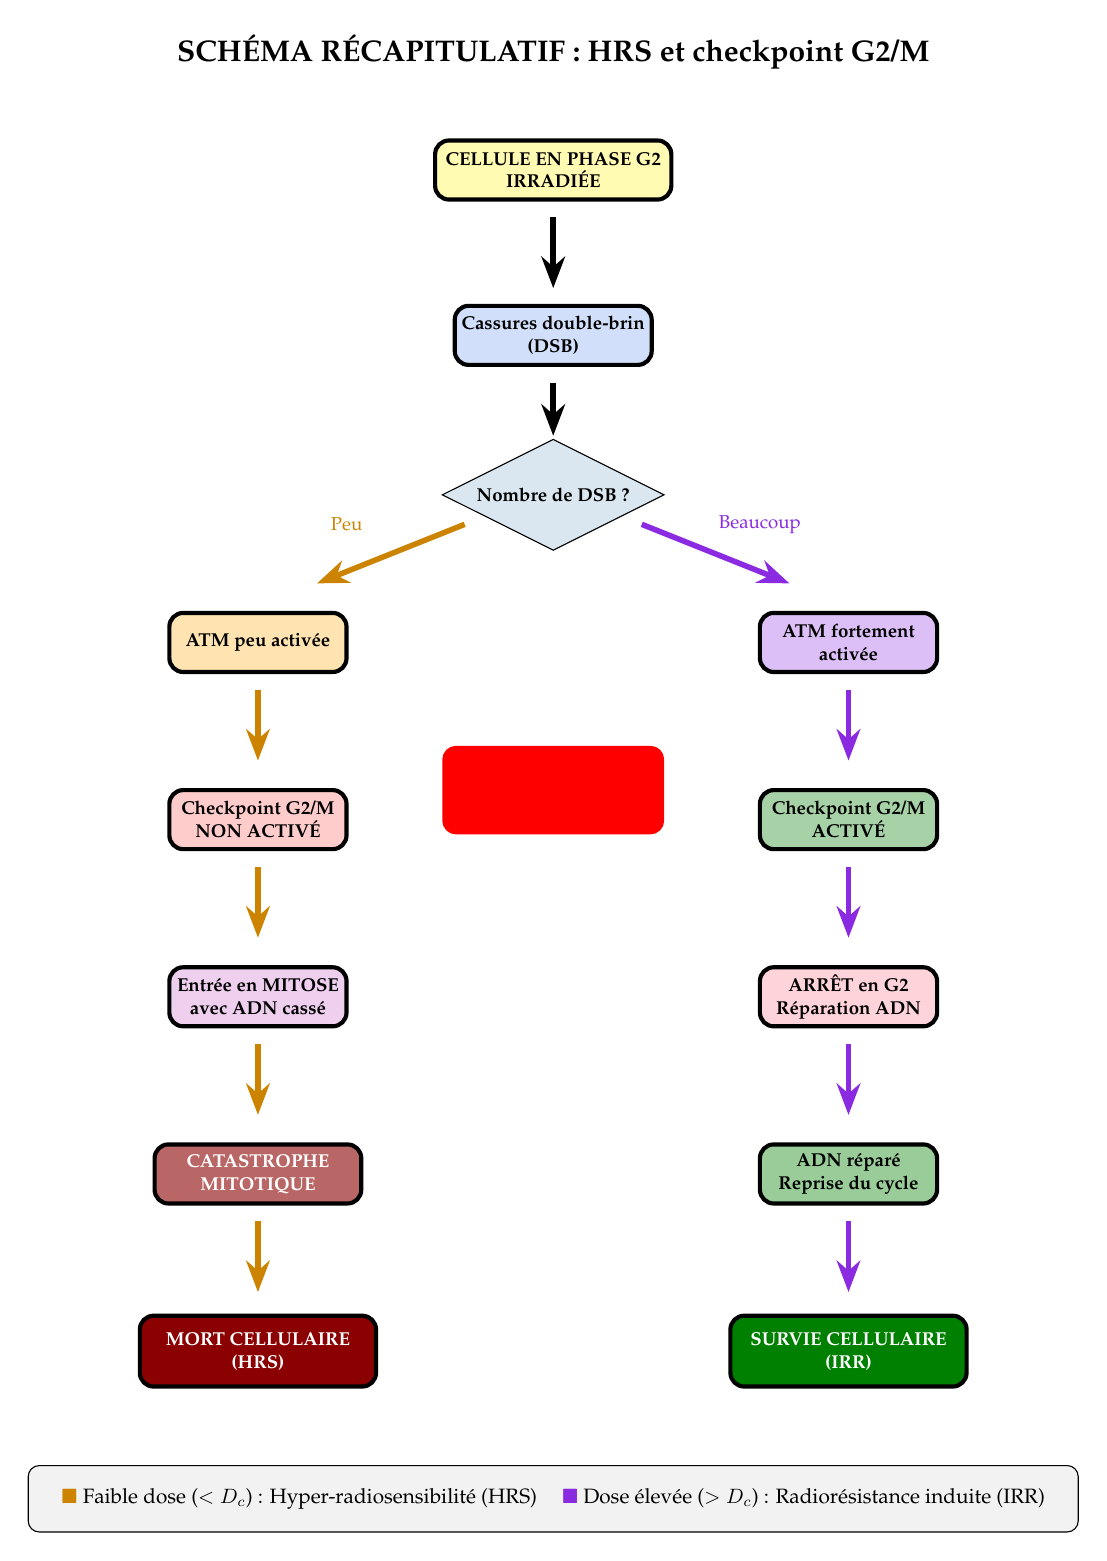
\begin{tikzpicture}[
    scale=0.75, 
    transform shape,
    box/.style={draw, rectangle, rounded corners=5pt, minimum width=3cm, minimum height=1cm, font=\small\bfseries, line width=1.5pt, align=center},
    arrow/.style={-{Stealth[length=4mm]}, line width=2pt}
]
    % Titre
    \node[font=\Large\bfseries] at (0,12) {SCHÉMA RÉCAPITULATIF : HRS et checkpoint G2/M};
    
    % Point de départ
    \node[box, fill=yellow!30, minimum width=4cm] (start) at (0,10) {CELLULE EN PHASE G2\\IRRADIÉE};
    
    % Branche
    \draw[arrow] (0,9.2) -- (0,8);
    \node[box, fill=dnacolor!30] (dsb) at (0,7.2) {Cassures double-brin\\(DSB)};
    
    % Division
    \draw[arrow] (0,6.4) -- (0,5.5);
    \node[draw, diamond, aspect=2, fill=atmcolor!20, minimum width=3cm, font=\small\bfseries] (decision) at (0,4.5) {Nombre de DSB ?};
    
    % === Branche GAUCHE (faible dose) ===
    \draw[arrow, lowdose!80!black] (-1.5,4) -- (-4,3);
    \node[font=\small, lowdose!80!black] at (-3.5,4) {Peu};
    
    \node[box, fill=lowdose!30] (low1) at (-5,2) {ATM peu activée};
    \draw[arrow, lowdose!80!black] (-5,1.2) -- (-5,0);
    
    \node[box, fill=red!20] (low2) at (-5,-1) {Checkpoint G2/M\\NON ACTIVÉ};
    \draw[arrow, lowdose!80!black] (-5,-1.8) -- (-5,-3);
    
    \node[box, fill=mcolor!50] (low3) at (-5,-4) {Entrée en MITOSE\\avec ADN cassé};
    \draw[arrow, lowdose!80!black] (-5,-4.8) -- (-5,-6);
    
    \node[box, fill=deathcolor!60, text=white, minimum width=3.5cm] (low4) at (-5,-7) {CATASTROPHE\\MITOTIQUE};
    \draw[arrow, lowdose!80!black] (-5,-7.8) -- (-5,-9);
    
    \node[box, fill=deathcolor, text=white, minimum width=4cm, minimum height=1.2cm] (death) at (-5,-10) {MORT CELLULAIRE\\(HRS)};
    
    % === Branche DROITE (dose élevée) ===
    \draw[arrow, highdose] (1.5,4) -- (4,3);
    \node[font=\small, highdose] at (3.5,4) {Beaucoup};
    
    \node[box, fill=highdose!30] (high1) at (5,2) {ATM fortement\\activée};
    \draw[arrow, highdose] (5,1.2) -- (5,0);
    
    \node[box, fill=checkcolor!40] (high2) at (5,-1) {Checkpoint G2/M\\ACTIVÉ};
    \draw[arrow, highdose] (5,-1.8) -- (5,-3);
    
    \node[box, fill=g2color!60] (high3) at (5,-4) {ARRÊT en G2\\Réparation ADN};
    \draw[arrow, highdose] (5,-4.8) -- (5,-6);
    
    \node[box, fill=survivecolor!40] (high4) at (5,-7) {ADN réparé\\Reprise du cycle};
    \draw[arrow, highdose] (5,-7.8) -- (5,-9);
    
    \node[box, fill=survivecolor, text=white, minimum width=4cm, minimum height=1.2cm] (survive) at (5,-10) {SURVIE CELLULAIRE\\(IRR)};
    
    % Encadré dose critique
    \node[draw, rectangle, rounded corners, fill=white, inner sep=8pt, line width=2pt, red] at (0,-0.5) {
        \begin{tabular}{c}
        \textbf{Dose critique $D_c$}\\
        $\approx 0.2 - 0.5$ Gy
        \end{tabular}
    };
    
    % Légende
    \node[draw, rectangle, rounded corners, fill=gray!10, inner sep=10pt] at (0,-12.5) {
        \begin{tabular}{ll}
        \textcolor{lowdose!80!black}{$\blacksquare$} Faible dose ($< D_c$) : Hyper-radiosensibilité (HRS) &
        \textcolor{highdose}{$\blacksquare$} Dose élevée ($> D_c$) : Radiorésistance induite (IRR)
        \end{tabular}
    };
\end{tikzpicture}
\captionsetup{labelformat=empty}
\caption{Schéma récapitulatif du rôle du checkpoint G2/M dépendant d'ATM dans le phénomène d'hyper-radiosensibilité. La dose critique $D_c$ détermine si le checkpoint est activé ou non.}
\end{figure}

\newpage

%==============================================================================
\normalsize 
\sectionbox{Conclusion}
\footnotesize 
%==============================================================================

\noindent Le checkpoint G2/M dépendant d'ATM joue un rôle central dans le phénomène d'hyper-radiosensibilité aux faibles doses :

\begin{enumerate}
    \item \textbf{ATM agit comme un senseur} des dommages à l'ADN, mais nécessite un seuil minimum de cassures pour s'activer efficacement.
    
    \item \textbf{Aux faibles doses} ($< D_c \approx 0.2-0.5$ Gy), le nombre de cassures est insuffisant pour activer pleinement ATM et le checkpoint G2/M.
    
    \item \textbf{Sans arrêt du cycle}, les cellules endommagées entrent en mitose avec des cassures non réparées, conduisant à la catastrophe mitotique et à la mort cellulaire.
    
    \item \textbf{Aux doses plus élevées}, ATM est activée, le checkpoint bloque les cellules en G2, permettant la réparation de l'ADN avant la mitose.
    
    \item Ce mécanisme explique le \textbf{paradoxe apparent} où les cellules survivent mieux à des doses modérées qu'à de très faibles doses.
\end{enumerate}


\normalsize 
\subsectionbox{Plages de doses caractéristiques}
\footnotesize 

\footnotesize
\noindent À mesure que la dose augmente au-delà d'environ 20--40~cGy, on observe une augmentation de la radiorésistance (\textbf{IRR}) jusqu'à ce que, au-delà d'environ 1~Gy, la radiorésistance soit maximale et que la survie cellulaire suive la courbe descendante habituelle décrite par le modèle \textbf{LQ}.

\begin{table}[h!]
\centering
\begin{tabular}{lcc}
\toprule
\footnotesize \textbf{Phase} & \footnotesize \textbf{Plage de dose} & \footnotesize \textbf{Caractéristique} \\
\midrule
\footnotesize \textbf{HRS} maximale & \footnotesize 5--20 cGy & \footnotesize Hypersensibilité marquée \\
\footnotesize Transition ($D_c$) & \footnotesize 20--40 cGy & \footnotesize Point d'inflexion \\
\footnotesize \textbf{IRR} & \footnotesize 40--100 cGy & \footnotesize Radiorésistance induite \\
\footnotesize Comportement \textbf{LQ} & \footnotesize $>$ 100 cGy & \footnotesize Modèle classique \\
\bottomrule
\end{tabular}
\caption{Plages de doses caractéristiques du phénomène \textbf{HRS}/\textbf{IRR}}
\end{table}


%==============================================================================
\normalsize 
\sectionbox{Modèles mathématiques}
\footnotesize 
%==============================================================================

\normalsize 
\subsectionbox{Modèle Linéaire-Quadratique (LQ)}
\footnotesize 

Le modèle LQ classique décrit la survie cellulaire par :
\begin{equation}
S = \exp(-\alpha D - \beta D^2)
\end{equation}
où $D$ est la dose, $\alpha$ représente les lésions létales directes et $\beta$ les lésions sub-létales accumulées.

\textbf{Limitation :} Ce modèle sous-estime la mort cellulaire aux faibles doses ($<$0.5~Gy).

\normalsize 
\subsectionbox{Modèle de Réparation Induite (IR)}
\footnotesize 

Le modèle IR, proposé par Joiner et al.~\cite{Joiner2001}, intègre le phénomène HRS/IRR :
\begin{equation}
\boxed{S = \exp\left\{-\alpha_r\left[1 + \left(\frac{\alpha_s}{\alpha_r} - 1\right)\exp\left(-\frac{D}{D_c}\right)\right]D - \beta D^2\right\}}
\end{equation}

\begin{table}[h!]
\centering
\begin{tabular}{clc}
\toprule
\textbf{Paramètre} & \textbf{Description} & \textbf{Valeurs typiques} \\
\midrule
$\alpha_s$ & Pente initiale (hypersensibilité) & 5--15 Gy$^{-1}$ \\
$\alpha_r$ & Pente à l'épaule (résistance) & 0.1--0.5 Gy$^{-1}$ \\
$D_c$ & Dose critique de transition & 0.2--0.5 Gy \\
$\beta$ & Composante quadratique & Variable \\
\bottomrule
\end{tabular}
\caption{Paramètres du modèle de Réparation Induite}
\end{table}

\textbf{Critères de confirmation de l'HRS :}
\begin{itemize}
    \item Rapport $\alpha_s/\alpha_r > 3$
    \item Intervalles de confiance de $\alpha_s$ et $\alpha_r$ non chevauchants
    \item $D_c \neq 0$
\end{itemize}

%==============================================================================
\normalsize 
\sectionbox{Mécanismes moléculaires}
\footnotesize 
%==============================================================================

\normalsize 
\subsectionbox{Rôle du checkpoint G2/M}
\footnotesize 

Le mécanisme principal de l'HRS implique une \textbf{défaillance du checkpoint G2/M} aux faibles doses~\cite{Marples2004} :

\begin{enumerate}
    \item \textbf{Faibles doses ($<D_c$)} : Le nombre de cassures double-brin (DSB) est insuffisant pour activer pleinement ATM
    \item \textbf{Checkpoint non activé} : Les cellules endommagées entrent en mitose avec de l'ADN non réparé
    \item \textbf{Catastrophe mitotique} : Mort cellulaire par apoptose ou nécrose
\end{enumerate}

\normalsize 
\subsectionbox{Cascade de signalisation ATM}
\footnotesize 

\begin{tcolorbox}[colback=green!5, colframe=green!50!black, title=Cascade de signalisation]
\begin{center}
DSB $\rightarrow$ ATM (activation) $\rightarrow$ Chk2 (phosphorylation) $\rightarrow$ Cdc25 (inhibition) $\rightarrow$ CDK1/CycB (blocage) $\rightarrow$ \textbf{ARRÊT G2}
\end{center}
\end{tcolorbox}

\textbf{Aux faibles doses :} ATM n'est pas suffisamment activée $\Rightarrow$ pas d'arrêt du cycle $\Rightarrow$ mort cellulaire accrue (HRS).

\textbf{Aux doses plus élevées :} ATM activée $\Rightarrow$ arrêt du cycle $\Rightarrow$ réparation de l'ADN $\Rightarrow$ survie améliorée (IRR).

%==============================================================================
\normalsize 
\sectionbox{Implications cliniques}
\footnotesize 
%==============================================================================

\begin{itemize}
    \item \textbf{Fractionnement ultra-hypofractionnée} : Exploiter l'HRS pour améliorer l'efficacité thérapeutique
    \item \textbf{Combinaison avec inhibiteurs de checkpoint} : Abolir l'IRR pour maintenir l'hypersensibilité
    \item \textbf{Protection des tissus sains} : Les tissus quiescents présentent moins d'HRS que les tumeurs proliférantes
\end{itemize}

\begin{comment}
\section{Modèle de Réparation Induite (Induced Repair Model - IR)}

\subsection{Hypothèse biologique}

Le modèle de réparation induite, développé par Joiner et Johns \cite{Joiner1988} puis affiné par Marples et Joiner \cite{Marples1993, Joiner1996}, repose sur l'hypothèse qu'un mécanisme de réparation protecteur est activé au-dessus d'une dose seuil $D_c$. En dessous de ce seuil, les cellules sont hypersensibles car le système de réparation n'est pas pleinement activé.

\subsection{Équation du modèle IR}

Le modèle IR modifie le paramètre $\alpha$ pour le rendre dose-dépendant:

\begin{equation}
\alpha(D) = \alpha_r \left[1 + \left(\frac{\alpha_s}{\alpha_r} - 1\right) \exp\left(-\frac{D}{D_c}\right)\right]
\label{eq:alpha_IR}
\end{equation}

L'équation complète de survie devient alors \cite{Joiner2001, Marples2008}:

\begin{equation}
\boxed{S = \exp\left\{-\alpha_r \left[1 + \left(\frac{\alpha_s}{\alpha_r} - 1\right) \exp\left(-\frac{D}{D_c}\right)\right] D - \beta D^2\right\}}
\label{eq:IR}
\end{equation}

où:
\begin{itemize}
    \item $\alpha_s$ = pente initiale à très faible dose (sensibilité accrue), typiquement 5--15 Gy$^{-1}$
    \item $\alpha_r$ = pente dans la région de l'épaule (résistance), typiquement 0.1--0.5 Gy$^{-1}$
    \item $D_c$ = dose critique de transition HRS $\rightarrow$ IRR, typiquement 0.2--0.5 Gy
    \item $\beta$ = composante quadratique (identique au modèle LQ)
\end{itemize}

\subsection{Critères de présence de l'HRS}

La présence de l'HRS est confirmée lorsque \cite{Krueger2010}:
\begin{enumerate}
    \item Les intervalles de confiance de $\alpha_s$ et $\alpha_r$ ne se chevauchent pas
    \item Le ratio $\alpha_s/\alpha_r > 1$ (typiquement $> 3$)
    \item $D_c$ est significativement différent de zéro
\end{enumerate}

\subsection{Comportement asymptotique}

\begin{itemize}
    \item Quand $D \rightarrow 0$: $\alpha(D) \rightarrow \alpha_s$ (hypersensibilité)
    \item Quand $D \gg D_c$: $\alpha(D) \rightarrow \alpha_r$ (résistance induite)
\end{itemize}

\section{Modèle de Réparation Induite Modifié (MIRM)}

Une version modifiée du modèle IR a été proposée pour améliorer l'ajustement aux données expérimentales \cite{Xue2016}:

\begin{equation}
\boxed{S = \exp\left\{-\alpha_r \left[1 + \left(\frac{\alpha_s}{\alpha_r} - 1\right) \exp\left(-\frac{D^2}{D_c^2}\right)\right] D - \beta D^2\right\}}
\label{eq:MIRM}
\end{equation}

Cette modification utilise une dépendance en $D^2/D_c^2$ plutôt qu'en $D/D_c$, ce qui peut mieux décrire certaines transitions HRS/IRR plus abruptes.

\section{Modèle à Réparation Variable (Variable IR Model)}

\subsection{Concept}

Dionet et collaborateurs \cite{Dionet2012} ont proposé un modèle considérant que la dose critique $D_c$ n'est pas uniforme dans la population cellulaire mais suit une distribution statistique. Cette approche reconnaît l'hétérogénéité intrinsèque des populations cellulaires.

\subsection{Formulation}

Si $f(D_c)$ représente la distribution de probabilité de la dose critique dans la population, la fraction de survie moyenne devient:

\begin{equation}
\boxed{\langle S \rangle = \int_0^{\infty} S(D, D_c) \cdot f(D_c) \, dD_c}
\label{eq:VIR}
\end{equation}

Une distribution log-normale ou gaussienne tronquée est souvent utilisée pour $f(D_c)$.

\section{Modèle basé sur la dynamique du checkpoint G2}

\subsection{Fondement biologique}

Ce modèle, développé par Olobatuyi, de Vries et Hillen \cite{Olobatuyi2018}, intègre explicitement la dynamique du checkpoint G2/M dans un système d'équations différentielles du cycle cellulaire.

\subsection{Système d'équations}

Le modèle utilise un système d'équations différentielles ordinaires (EDO) décrivant les populations cellulaires dans chaque phase du cycle:

\begin{equation}
\begin{cases}
\dfrac{dG_1}{dt} = 2k_M \cdot M - k_{G_1} \cdot G_1 \\[10pt]
\dfrac{dS}{dt} = k_{G_1} \cdot G_1 - k_S \cdot S \\[10pt]
\dfrac{dG_2}{dt} = k_S \cdot S - k_{G_2}(D) \cdot G_2 \\[10pt]
\dfrac{dM}{dt} = k_{G_2}(D) \cdot G_2 - k_M \cdot M
\end{cases}
\label{eq:G2model}
\end{equation}

où $k_{G_2}(D)$ est le taux de transition G2$\rightarrow$M dépendant de la dose, modélisant l'activation du checkpoint.

\subsection{Relation avec le ratio $\alpha_s/\alpha_r$}

Les auteurs ont dérivé une formule explicite reliant le ratio d'hypersensibilité à la fraction de survie à 2 Gy (SF2):

\begin{equation}
\boxed{\frac{\alpha_s}{\alpha_r} = f(SF_2, \text{paramètres du checkpoint})}
\label{eq:ratio_SF2}
\end{equation}

Cette relation logarithmique confirme le lien entre HRS/IRR et la radiosensibilité aux doses cliniquement pertinentes \cite{Alsbeih2013}.

\section{Modèle Microdosiométrique-Cinétique (MK Model)}

\subsection{Principe}

Le modèle microdosiométrique-cinétique (MK), développé par Hawkins \cite{Hawkins1994} et adapté par Matsuya et collaborateurs \cite{Matsuya2017}, considère la distribution stochastique de l'énergie déposée à l'échelle subcellulaire.

\subsection{Équation fondamentale}

\begin{equation}
\boxed{S = \exp\left[-(\alpha_0 + \beta z_1^*) D - \beta D^2\right]}
\label{eq:MK}
\end{equation}

où:
\begin{itemize}
    \item $\alpha_0$ = composante linéaire intrinsèque
    \item $z_1^*$ = dose spécifique moyenne par événement unique
    \item $\beta$ = composante quadratique
\end{itemize}

\subsection{Extension MK-DNA}

Le modèle MK-DNA \cite{Matsuya2017} incorpore les variations de contenu en ADN pendant l'irradiation:

\begin{equation}
\alpha_{MK-DNA}(t) = \alpha_0 \cdot \frac{\langle DNA(t) \rangle}{\langle DNA_0 \rangle}
\label{eq:MK_DNA}
\end{equation}

où $\langle DNA(t) \rangle$ représente la quantité moyenne d'ADN par noyau au temps $t$, tenant compte de l'accumulation des cellules en phase G2.

\section{Modèle Intégré Microdosiométrique-Cinétique (IMK)}

\subsection{Intégration des effets non-ciblés}

Le modèle IMK \cite{Matsuya2018} étend le modèle MK en incorporant les effets bystander (non-ciblés):

\begin{equation}
\boxed{S_{IMK} = S_{TE} \cdot S_{NTE}}
\label{eq:IMK}
\end{equation}

où:
\begin{itemize}
    \item $S_{TE}$ = survie due aux effets ciblés (targeted effects)
    \item $S_{NTE}$ = survie due aux effets non-ciblés (non-targeted effects)
\end{itemize}

\subsection{Contribution à l'HRS}

Le modèle IMK attribue l'HRS à la combinaison de:
\begin{enumerate}
    \item L'induction de cassures double-brin (DSB) par les signaux intercellulaires
    \item La faible efficacité de réparation de l'ADN dans les cellules non-touchées
\end{enumerate}

\section{Modèle du Principe de Charge Mutationnelle Minimale}

\subsection{Hypothèse}

Madas \cite{Madas2019} a proposé un modèle basé sur l'hypothèse que le système cellulaire optimise la fraction de survie pour minimiser la charge mutationnelle totale dans le tissu.

\subsection{Formulation}

Pour chaque dose $D$, la fraction de survie optimale $S^*(D)$ est celle qui minimise le nombre total de mutations:

\begin{equation}
\boxed{S^*(D) = \arg\min_S \left[ N_0 \cdot S \cdot \mu(D) + N_0 \cdot (1-S) \cdot \mu_{div} \right]}
\label{eq:MMM}
\end{equation}

où:
\begin{itemize}
    \item $N_0$ = nombre initial de cellules
    \item $\mu(D)$ = taux de mutation radio-induit
    \item $\mu_{div}$ = taux de mutation spontané par division cellulaire
\end{itemize}

Ce modèle prédit que l'HRS est plus prononcé dans les lignées cellulaires avec des défauts de réparation de l'ADN.

\section{Modèle RCR (Repairable-Conditionally Repairable)}

Le modèle RCR \cite{Lind2003} propose une alternative au modèle IR:

\begin{equation}
\boxed{S = \exp(-aD) + bD \cdot \exp(-cD)}
\label{eq:RCR}
\end{equation}

où $a$, $b$ et $c$ sont des paramètres ajustables. Ce modèle ne fournit pas directement $\alpha_s$ et $\alpha_r$ mais peut décrire certaines courbes HRS/IRR avec moins de paramètres.

\section{Modèle pour la leucémie myéloïde aiguë (rAML)}

\subsection{Application de l'HRS à la carcinogenèse}

Stouten et collaborateurs \cite{Stouten2022} ont développé un modèle mathématique mécanistique intégrant l'HRS pour prédire l'incidence de leucémie myéloïde aiguë radio-induite (rAML) chez la souris CBA.

\subsection{Équations du modèle}

Le modèle utilise un système de trois équations différentielles pour les populations de cellules normales ($N$), intermédiaires ($I$) et malignes ($M$):

\begin{equation}
\begin{cases}
\dfrac{dN}{dt} = -\delta_N(D) \cdot N - \mu_{del}(D) \cdot N \\[10pt]
\dfrac{dI}{dt} = \mu_{del}(D) \cdot N - \delta_I(D) \cdot I + r_I \cdot I - \mu_{pt} \cdot I \\[10pt]
\dfrac{dM}{dt} = \mu_{pt} \cdot I
\end{cases}
\label{eq:rAML}
\end{equation}

où les taux de mort cellulaire $\delta(D)$ incorporent l'effet HRS via le modèle IR.

\section{Tableau récapitulatif des modèles}

\begin{table}[h!]
\centering
\caption{Comparaison des modèles mathématiques pour l'HRS}
\label{tab:comparaison}
\begin{tabular}{p{3.5cm}p{2cm}p{5cm}p{3cm}}
\toprule
\textbf{Modèle} & \textbf{Paramètres} & \textbf{Caractéristiques} & \textbf{Référence} \\
\midrule
IR (Induced Repair) & $\alpha_s$, $\alpha_r$, $D_c$, $\beta$ & Standard pour l'HRS & \cite{Joiner2001} \\
\addlinespace
Variable IR & + distribution de $D_c$ & Hétérogénéité cellulaire & \cite{Dionet2012} \\
\addlinespace
G2-checkpoint & EDO cycle cellulaire & Mécanistique & \cite{Olobatuyi2018} \\
\addlinespace
MK-DNA & Microdosimétriques & Contenu ADN variable & \cite{Matsuya2017} \\
\addlinespace
IMK & + effets bystander & Effets non-ciblés & \cite{Matsuya2018} \\
\addlinespace
Charge mutationnelle & Taux de mutation & Optimisation évolutive & \cite{Madas2019} \\
\addlinespace
RCR & $a$, $b$, $c$ & Formulation alternative & \cite{Lind2003} \\
\bottomrule
\end{tabular}
\end{table}

\section{Paramètres typiques du modèle IR}

\begin{table}[h!]
\centering
\caption{Valeurs typiques des paramètres du modèle IR pour différentes lignées cellulaires}
\label{tab:parametres}
\begin{tabular}{lccccc}
\toprule
\textbf{Lignée cellulaire} & $\alpha_s$ (Gy$^{-1}$) & $\alpha_r$ (Gy$^{-1}$) & $\alpha_s/\alpha_r$ & $D_c$ (Gy) & \textbf{Réf.} \\
\midrule
V79 (hamster) & 8.9 & 0.24 & 37.1 & 0.31 & \cite{Marples1993} \\
T98G (gliome) & 11.0 & 0.15 & 73.3 & 0.25 & \cite{Short1999} \\
HeLa (col utérin) & 11.0 & 1.55 & 7.1 & 0.28 & \cite{Das2015} \\
MR4 (fibroblaste) & 5.2 & 0.18 & 28.9 & 0.41 & \cite{Krueger2010} \\
A549 (poumon) & 9.5 & 0.31 & 30.6 & 0.35 & \cite{Dai2009} \\
\bottomrule
\end{tabular}
\end{table}

\section{Conclusion}

Les modèles mathématiques de l'HRS ont évolué depuis le modèle empirique de réparation induite vers des approches plus mécanistiques intégrant la dynamique du cycle cellulaire, la microdosiométrie et les effets non-ciblés. Le modèle IR reste le plus utilisé en pratique pour sa simplicité et sa capacité à extraire des paramètres biologiquement interprétables ($\alpha_s$, $\alpha_r$, $D_c$). Les modèles plus récents offrent une meilleure compréhension des mécanismes sous-jacents et permettent d'explorer les implications de l'HRS pour la radiothérapie et l'évaluation des risques aux faibles doses.

\end{comment}


\newpage
\appendix
\section{\color{blue}\textbf{Joiner MC, Johns H (1988)}\color{black}}
\label{sec:resume1}
\medskip

\begin{tcolorbox}[colback=blue!5,colframe=blue,title=\textbf{Radiat Res., Vol.114(2), pp.385-98, 1988\\
Renal damage in the mouse: the response to very small doses per fraction\\
M C Joiner, H Johns}]
\footnotesize

\noindent Experiments were undertaken to study the effect on the mouse kidney of repeated X-ray doses in the range 0.2 to 1.6 Gy per fraction and neutron doses in the range 0.05 to 0.25 Gy per fraction. A top-up design of experiment was used, so that additional graded doses of d(4)-Be neutrons ($\bm{EN}$ = 2.3 MeV) were given to bring the subthreshold damage produced by these treatments into the measurable range. This approach avoided the necessity to use a large number of fractions to study low doses per fraction. Renal damage was assessed using three methods: 51Cr-EDTA clearance, urine output, and hematocrit at 16-50 weeks postirradiation. The dose-response curves obtained were resolved best at 29 weeks. However, the results were also examined by fitting second-order polynomials to the data for response versus time postirradiation and using interpolated values from these functions at 29 weeks to construct dose-response curves. This method reduced slightly the variation in the dose-response data, but the interrelationship between the dose-response curves remained the same. The data were used to test the linear-quadratic ($LQ$) description of the underlying X-ray dose-fractionation relationship. The model fits well down to X-ray doses per fraction of approximately 1 Gy, but lower X-ray doses were more effective per gray than predicted by $LQ$, as seen previously in skin [M. C. Joiner et al., Int. J. Radiat. Biol. 49, 565-580 (1986)]. This increased X-ray effectiveness and deviation from LQ are reflected directly in a decrease in the RBE of d(4)-Be neutrons relative to X-rays at low doses, since the underlying response to these neutrons is linear in this low-dose region. The RBE decreases from 9.9 to 4.7 as the X-ray dose per fraction is reduced below 0.8 Gy to 0.2 Gy, reflecting an increase in X-ray effectiveness by a factor of 2.1. A model is discussed which attempts to explain this behavior at low doses per fraction.

\begin{center}
    \includegraphics[width=0.8\linewidth]{Figures/Joiner_RadRes_1988.png}
    %\captionof{figure}{Schéma de l’expérience}
\end{center}
\end{tcolorbox}

\section{\color{blue}\textbf{Marples B, Joiner MC (1993)}\color{black}}
\label{sec:resume2}
\medskip

\begin{tcolorbox}[colback=blue!5,colframe=blue,title=\textbf{Radiation Research, Vol.133(1), pp.41-51, 1993\\
The response of Chinese hamster V79 cells to low radiation doses: evidence of enhanced sensitivity of the whole cell population\\
B Marples, M C Joiner}]
\footnotesize

\noindent High-resolution measurements of the survival of asynchronous Chinese hamster V79-379A cells in vitro after single doses of X rays (0.01-10.0 Gy) and neutrons (0.02-3.0 Gy) were made using a computerized microscope for locating and identifying cells (Palcic and Jaggi, Int. J. Radiat. Biol. 50, 345-352, 1986). The X-ray response from 1 to 10 Gy showed a good fit to a linear-quadratic (LQ) dose-survival model, but with X-ray doses below 0.6 Gy, an increased X-ray effectiveness was observed, with cell survival below the prediction made from the data above 1 Gy using the LQ model. The effect per unit dose (-log(e)SF/dose) increased by a factor of approximately 2, from 0.19 Gy-1 at a dose of 1 Gy to 0.37 Gy-1 at a dose of 0.1 Gy. This phenomenon was not seen with neutrons, and cell survival decreased exponentially over the whole neutron dose range studied. Further data suggest that this phenomenon is unlikely to be due to a subpopulation of X-ray-sensitive cells determined either genetically or phenotypically by distribution of the population within the cell cycle. The existence of low-dose sensitivity also appeared to be independent of dose rate in the range 0.016-1.7 Gy min-1. A possible explanation of these results is that the phenomenon reflects "induced repair" or a stress response: low doses in vitro (or low doses per fraction in vivo) are more effective per gray than higher doses because only at the higher doses is there sufficient damage to trigger repair systems or other radioprotective mechanisms. 

\begin{center}
    \includegraphics[width=0.5\linewidth]{Figures/Marples_RadRes_1993.png}
    %\captionof{figure}{Schéma de l’expérience}
\end{center}

\end{tcolorbox}

\section{\color{blue}\textbf{P Lambin, B Marples, B Fertil, E P Malaise, M C Joiner (1993)}\color{black}}
\label{sec:resume3}
\medskip

\begin{tcolorbox}[colback=blue!5,colframe=blue,title=\textbf{Int J Radiat Biol.,Vol.63(5), pp.639-50, 1993\\
Hypersensitivity of a human tumour cell line to very low radiation doses\\
P Lambin, B Marples, B Fertil, E P Malaise, M C Joiner}]
\footnotesize

\noindent Survival of HT29 cells was measured after irradiation with single doses of X-rays (0.05-5 Gy) and neutrons (0.025-1.5 Gy), using a Dynamic Microscopic Imaging Processing Scanner (DMIPS) with which individual cells can be accurately located in tissue culture flasks, their positions recorded, and after an appropriate incubation time the recorded positions revisited to allow the scoring of survivors. The response over the X-ray dose range 2-5 Gy showed a good fit to a Linear-Quadratic (LQ) model. For X-ray doses below 1 Gy, an increased X-ray effectiveness was observed with cell survival below the high-dose LQ prediction. The value of --dose/loge (SF) for each experimental data point, plotted against dose, demonstrated clearly how X-rays are maximally effective at doses approaching zero, becoming less effective as the dose increases and with minimal effectiveness at about 0.6 Gy then becoming more effective again as the dose increases above 1.5 Gy. This phenomenon was not seen with neutrons. Neutron RBE was calculated for each X-ray data point by taking each X-ray survival value and comparing it with the common LQ fit to all the neutron data. Over the X-ray dose range 0.05-0.2 Gy, the RBE is close to 1 indicating that these very low doses of X-rays are of similar effectiveness to neutrons in killing cells. The increase in RBE with increasing dose over the range 0.05-1 Gy, and the slight decrease in RBE above 1 Gy, reflect primarily the changes in X-ray sensitivity over the whole dose range of 0.05-5 Gy. Several arguments suggest that this phenomenon could reflect an induced radioresistance so that in this system low single doses of X-rays are more effective per Gy than higher doses in reducing cell survival because only at higher doses, above a threshold, is there sufficient damage to trigger radioprotective mechanisms.

\end{tcolorbox}


\section{\color{blue}\textbf{E P Malaise,~P Lambin,~M C Joiner (1994)}\color{black}}
\label{sec:resume4}
\medskip

\begin{tcolorbox}[colback=blue!5,colframe=blue,title=\textbf{Radiat Res., Vol.138(1 Suppl),pp.S25-7, 1994\\
Radiosensitivity of human cell lines to small doses. Are there some clinical implications?\\
E P Malaise,~P Lambin,~M C Joiner}]
\footnotesize
\noindent The concept of intrinsic radiosensitivity is now strongly associated with the linear-quadratic ($LQ$) model which is currently the best and the most reliable method to fit the first three decades of a survival curve for both human fibroblast and human tumor cell lines. This approach has led to the major conclusions that it is the initial part, and not the distal part, of the survival curve which truly characterizes intrinsic cellular radiosensitivity and there is a correlation between the parameters describing mainly the initial part of the survival curve ($\alpha$, $SF2$, $D$) and the clinical radioresponsiveness. More accurate analysis with flow cytometry or a dynamic microscopic image processing scanner ($DMIPS$) has allowed further study of the survival curve which has shown two sorts of substructure. On one hand, the overall survival curve of exponentially growing cells is described by two or more sets of alpha, beta parameters (heterogeneity in radiosensitivity due to the cell cycle). On the other hand, hypersensitivity at very low doses ($\mathrm{<}$ 0.5 Gy) followed by an increase of the radioresistance of the whole population at higher doses has also been observed. This phenomenon is not described by the conventional $LQ$ model and has been interpreted as an induced radioresistance which seems to be negatively correlated with intrinsic radiosensitivity. In clinical radiotherapy, there are two sorts of response of normal tissues: (1) the early and late damage and (2) the carcinogenesis. Concerning the first point, the clinically detectable radiation damage appears at doses usually around 20 Gy (in 2-Gy fractions) with the exception of the hemopoietic and the lymphatic tissues. Therefore, the small doses delivered at the edges or in the penumbrae of treatment fields in routine radiotherapy cannot create detectable damage, despite a potentially much higher effect per unit dose, because the total doses are still very small. However, it may be important to bear in mind the possible extra effect of low doses outside the target volume if regions in the vicinity are subsequently retreated. Concerning clinical radiation-induced carcinogenesis, three studies described a higher relative risk associated with small doses per fraction or very low dose rate. The results and the interpretation of these studies are discussed. 
\end{tcolorbox}

\section{\color{blue}\textbf{P. Lambin, B. Fertil, E. P. Malaise, M. C. Joiner (1994)}\color{black}}
\label{sec:resume5}
\medskip

\begin{tcolorbox}[colback=blue!5,colframe=blue,title=\textbf{Radiation Research, Vol.138(1), 1994\\
Multiphasic Survival Curves for Cells of Human Tumor Cell Lines: Induced Repair or Hypersensitive Subpopulation?\\
P. Lambin, B. Fertil, E. P. Malaise, M. C. Joiner}]
\footnotesize
\noindent Survival of the cells of three human tumor cell lines of differing radiosensitivity was measured after irradiation with single doses of X rays (0.05-5 Gy). At doses below 1 Gy, cells were more radiosensitive than predicted by back-extrapolating the high-dose response. This difference was more marked for cells of the radioresistant cell lines than the radiosensitive cell line so that the "true" initial slopes of the survival curves, at very low doses, were similar for the cells of the three cell lines. This phenomenon could reflect an induced radioresistance so that low doses of X rays are more effective per gray than higher doses, because only at higher doses is there sufficient damage to trigger repair systems or other radioprotective mechanisms which can then act during the time course for repair of DNA injury
\begin{center}
    \includegraphics[width=0.5\linewidth]{Figures/Lambin_RadRes_1994.png}
\end{center}
\end{tcolorbox}

\section{\color{blue}\textbf{B G Wouters ,~L D Skarsgard (1994)}\color{black}}
\label{sec:resume6}
\medskip

\begin{tcolorbox}[colback=blue!5,colframe=blue,title=\textbf{Radiat Res., Vol.138(1 Suppl), pp.S76-80, 1994\\
The response of a human tumor cell line to low radiation doses: evidence of enhanced sensitivity\\
B G Wouters ,~L D Skarsgard}]
\footnotesize
\noindent The survival of asynchronous, exponentially growing DU-145 human tumor cells was measured after single doses of X rays in the dose range of 0.05-4 Gy using the cell sorting assay. When the response was modeled with the linear-quadratic (LQ) equation, a good fit to the data was observed for dose levels above 1 Gy; however, a region of enhanced sensitivity was observed at doses less than this. One possible explanation of this low-dose substructure is that a small, sensitive subpopulation of cells is selectively killed at low doses. Modeling of the radiation response with a two-population LQ model suggests that for these data this explanation is unlikely. Another possibility is that the whole cell population is initially hypersensitive, becoming radioresistant as damage is sustained by the cell. Conceivably this radioprotective mechanism could act in one of two ways. The cell could move from a radiation-sensitive to a radiation-resistant state by a continuous function of dose, or alternatively, only after a sufficient accumulation of damage, i.e. a "triggering dose." Both of these possibilities have been explored in the results of fitting two "induced resistance" models. 

\begin{center}
    \includegraphics[width=0.5\linewidth]{Figures/Wouters_RadRes_1994.png}
\end{center}
\end{tcolorbox}

\section{\color{blue}\textbf{Marples B, Adomat H, Koch CJ, Skov KA (1996)}\color{black}}
\label{sec:resume7}
\medskip

\begin{tcolorbox}[colback=blue!5,colframe=blue,title=\textbf{Int J Radiat Biol., Vol.70(4),pp. 429-36, 1996\\
Response of V79 cells to low doses of X-rays and negative pi-mesons: clonogenic survival and DNA strand breaks\\
B Marples, H Adomat,~C J Koch,~K A Skov}]
\footnotesize
\noindent Mammalian cells are hypersensitive to very low doses of X-rays ($\mathrm{<}$ 0.2 Gy), a response which is followed by increased radioresistance up to 1 Gy. Increased radioresistance is postulated to be a response to DNA damage, possibly single-strand breaks, and it appears to be a characteristic of low linear energy transfer (LET) radiation. Here we demonstrate a correspondence between the extent of the increased radioresistance and linear energy transfer of 250 kVp X-rays and plateau and Bragg peak negative pi-mesons. The results support our hypothesis since the size of the increased radioresistant response appears to correspond to the number of radiation induced single-strand breaks. Furthermore, since survival prior to the increased radioresistant response ($\mathrm{<}$ 0.2 Gy) was LET-independent, these data support the notion that the increased radioresistant response may dictate the overall survival response to higher doses. However, while these data provide further circumstantial evidence for the involvement of DNA strand breaks in the triggering of increased radioresistance, more direct conclusions cannot be made. The data are not accurate enough to detect structure in the single-strand break profiles, the production of single-strand breaks being apparently linear with dose

%\begin{center}
%    \includegraphics[width=0.5\linewidth]{Figures/Wouters_RadRes_1994.png}
%\end{center}
\end{tcolorbox}

\section{\color{blue}\textbf{B G Wouters,~A M Sy,~L D Skarsgard (1996)}\color{black}}
\label{sec:resume8}
\medskip

\begin{tcolorbox}[colback=blue!5,colframe=blue,title=\textbf{Radiat Res., Vol.146(4), pp.399-413, 1996\\
Low-dose hypersensitivity and increased radioresistance in a panel of human tumor cell lines with different radiosensitivity\\
B G Wouters,~A M Sy,~L D Skarsgard}]
\footnotesize
\noindent It is well known that cells of human tumor cell lines display a wide range of sensitivity to radiation, at least a part of which can be attributed to different capacities to process and repair radiation damage correctly. We have examined the response to very low-dose radiation of cells of five human tumor cell lines that display varying sensitivity to radiation, using an improved assay for measurement of radiation survival. This assay improves on the precision of conventional techniques by accurately determining the numbers of cells at risk, and has allowed us to measure radiation survival to doses as low as 0.05 Gy. Because of the statistical limitations in measuring radiation survival at very low doses, extensive averaging of data was used to determine the survival response accurately. Our results show that the four most resistant cell lines exhibit a region of initial low-dose hypersensitivity. This hypersensitivity is followed by an increase in radioresistance over the dose range 0.3 to 0.7 Gy, beyond which the response is typical of that seen in most survival curves. Mathematical modeling of the responses suggests that this phenomenon is not due to a small subpopulation of sensitive cells (e.g. mitotic), but rather is a reflection of the induction of resistance in the whole cell population, or at least a significant proportion of the whole cell population. These results suggest that a dose-dependent alteration in the processing of DNA damage over the initial low-dose region of cell survival may contribute to radioresistance in some cell lines. 
%\begin{center}
%    \includegraphics[width=0.5\linewidth]{Figures/Wouters_RadRes_1994.png}
%\end{center}
\end{tcolorbox}

\section{\color{blue}\textbf{L D Skarsgard,~M W Skwarchuk,~B G Wouters,~R E Durand (1996)}\color{black}}
\label{sec:resume9}
\medskip

\begin{tcolorbox}[colback=blue!5,colframe=blue,title=\textbf{Radiat Res., Vol.146(4), pp.388-98, 1996 1996\\
Substructure in the radiation survival response at low dose in cells of human tumor cell lines\\
L D Skarsgard,~M W Skwarchuk,~B G Wouters,~R E Durand}]
\footnotesize
\noindent In earlier studies using asynchronously growing Chinese hamster cells, we observed substructure in the survival response at low doses. The substructure appeared to result from subpopulations of cells having different, cell cycle phase-dependent radiosensitivity. We have now applied the same flow cytometry and cell sorting technique to accurately measure the responses of cells of eight different asynchronously growing human tumor cell lines, representing a wide range in radiosensitivity. When the data were fitted with a linear-quadratic (LQ) function, most of these lines showed substructure similar to that observed in Chinese hamster cells, with the result that values of alpha and beta were dependent on the dose range used for fitting. Values of alpha describing the low-dose response were typically smaller (by as much as 2.2 times) than the alpha describing the high-dose response, while values of beta were larger at low doses. Values of alpha/beta from our measurements are in reasonable agreement with other values published recently if we fit the data for the high-dose range (excluding, for example, 0-4 Gy), which corresponds to a conventional survival response measurement. However, the values of alpha/beta describing the low-dose range were, on average, 2.8-fold smaller. The results show that the usual laboratory measurement of cell survival over 2 or 3 logs of cell killing, if fitted with a single LQ function, will yield alpha and beta values which may give a rather poor description of cell inactivation at low dose in asynchronous cells, no matter how carefully those measurements are done, unless the low-dose range is fitted separately. The contribution of killing represented by the beta coefficient at low doses was found to be surprisingly large, accounting for 40-70\% of cell inactivation at 2 Gy in these cell lines. A two-population LQ model provides excellent fits to the data for most of the cell lines though, as one might expect with a five-parameter model, the best-fitting value of the various parameters is far from unique, and the values are probably not reliable indicators of the size and radiosensitivity of the different cell subpopulations. At very low dose, below 0.5-1 Gy, another order of substructure is observed: the hypersensitive response; this is described in the accompanying paper (Wouters et al., Radiat. Res. 146, 399-413, 1996). 
%\begin{center}
%    \includegraphics[width=0.5\linewidth]{Figures/Wouters_RadRes_1994.png}
%\end{center}
\end{tcolorbox}

\section{\color{blue}\textbf{L D Skarsgard, M W Skwarchuk,~B G Wouters,~R E Durand (1996)}\color{black}}
\label{sec:resume10}
\medskip

\begin{tcolorbox}[colback=blue!5,colframe=blue,title=\textbf{Radiat Res., Vol.146(4), pp.388-98, 1996\\
Substructure in the radiation survival response at low dose in cells of human tumor cell lines\\
L D Skarsgard, M W Skwarchuk,~B G Wouters,~R E Durand }]
\footnotesize
\noindent In earlier studies using asynchronously growing Chinese hamster cells, we observed substructure in the survival response at low doses. The substructure appeared to result from subpopulations of cells having different, cell cycle phase-dependent radiosensitivity. We have now applied the same flow cytometry and cell sorting technique to accurately measure the responses of cells of eight different asynchronously growing human tumor cell lines, representing a wide range in radiosensitivity. When the data were fitted with a linear-quadratic (LQ) function, most of these lines showed substructure similar to that observed in Chinese hamster cells, with the result that values of alpha and beta were dependent on the dose range used for fitting. Values of alpha describing the low-dose response were typically smaller (by as much as 2.2 times) than the alpha describing the high-dose response, while values of beta were larger at low doses. Values of alpha/beta from our measurements are in reasonable agreement with other values published recently if we fit the data for the high-dose range (excluding, for example, 0-4 Gy), which corresponds to a conventional survival response measurement. However, the values of alpha/beta describing the low-dose range were, on average, 2.8-fold smaller. The results show that the usual laboratory measurement of cell survival over 2 or 3 logs of cell killing, if fitted with a single LQ function, will yield alpha and beta values which may give a rather poor description of cell inactivation at low dose in asynchronous cells, no matter how carefully those measurements are done, unless the low-dose range is fitted separately. The contribution of killing represented by the beta coefficient at low doses was found to be surprisingly large, accounting for 40-70\% of cell inactivation at 2 Gy in these cell lines. A two-population LQ model provides excellent fits to the data for most of the cell lines though, as one might expect with a five-parameter model, the best-fitting value of the various parameters is far from unique, and the values are probably not reliable indicators of the size and radiosensitivity of the different cell subpopulations. At very low dose, below 0.5-1 Gy, another order of substructure is observed: the hypersensitive response; this is described in the accompanying paper (Wouters et al., Radiat. Res. 146, 399-413, 1996). 
%\begin{center}
%    \includegraphics[width=0.5\linewidth]{Figures/Wouters_RadRes_1994.png}
%\end{center}
\end{tcolorbox}

%==============================================================================
% BIBLIOGRAPHIE
%==============================================================================

\begin{thebibliography}{299}






















\bibitem{Alsbeih2013}
Alsbeih G, Al-Meer RS, Al-Harbi N, et al.
\textit{A Logarithmic Formula to Describe the Relationship between the Increased Radiosensitivity at Low Doses and the Survival at 2 Gray.}
Sultan Qaboos Univ Med J. 2013;13(4):538-543.

\bibitem{AlMayah2022}
Al-Mayah A, Irons SL, Mothersill C, Kadhim M.
\textit{Genomic instability in non-targeted human cells.}
Mutat Res. 2022;823:111756.

\bibitem{Andaur2018}
Andaur R, Morales D, Fernández M.
\textit{Low-dose hyper-radiosensitivity in colorectal cancer cells: role of DNA damage response.}
Radiat Oncol. 2018;13:89.

\bibitem{Bakkenist2003}
Bakkenist CJ, Kastan MB.
\textit{DNA damage activates ATM through intermolecular autophosphorylation and dimer dissociation.}
Nature. 2003;421(6922):499-506.

\bibitem{Cerri2019}
Cerri M, Tinganelli W, Negrini M, et al.
\textit{Hibernation for space travel: impact on radioprotection.}
Life Sci Space Res. 2016;11:1-9.

\bibitem{Cerri2019b}
Cerri M, et al.
\textit{Hibernation and radioprotection: gene expression in the liver and testicle of rats irradiated under synthetic torpor.}
Int J Mol Sci. 2019;20(2):352.

\bibitem{CANHR2019}
Center for Alaska Native Health Research (CANHR).
\textit{Hibernation and DNA Repair.}
University of Alaska Fairbanks. 2019-2024.

\bibitem{Choukèr2019}
Choukèr A, et al.
\textit{European Space Agency's hibernation (torpor) strategy for deep space missions: linking biology to engineering.}
Neurosci Biobehav Rev. 2019;131:618-626.

\bibitem{Carey2003}
Carey HV, Andrews MT, Martin SL.
\textit{Mammalian hibernation: cellular and molecular responses to depressed metabolism and low temperature.}
Physiol Rev. 2003;83(4):1153-1181.

\bibitem{Collis2004}
Collis SJ, Schwaninger JM, Ntambi AJ, et al.
\textit{Evasion of early cellular response mechanisms following low level radiation-induced DNA damage.}
J Biol Chem. 2004;279(48):49624-49632.

\bibitem{Dai2009}
Dai X, Tao D, Wu H, Cheng J.
\textit{Low dose hyper-radiosensitivity in human lung cancer cell line A549 and its possible mechanisms.}
J Huazhong Univ Sci Technolog Med Sci. 2009;29(1):101-106.

\bibitem{Das2015}
Das S.
\textit{Radiobiological response of cervical cancer cell line in low dose region: evidence of low dose hypersensitivity (HRS) and induced radioresistance (IRR).}
J Clin Diagn Res. 2015;9(7):XC01-XC04.

\bibitem{Dionet2012}
Dionet C, Müller-Barthélémy M, Marceau G, et al.
\textit{Low-dose radiation hyper-radiosensitivity in multicellular tumour spheroids.}
Br J Radiol. 2012;85(1018):e823-e830.

\bibitem{Drew2007}
Drew KL, Buck CL, Barnes BM, Christian SL, Rasley BT, Harris MB.
\textit{Central nervous system regulation of mammalian hibernation: implications for metabolic suppression and ischemia tolerance.}
J Neurochem. 2007;102(6):1713-1726.

\bibitem{Ghosh2017}
Ghosh S, Indracanti N, Bhattacharya J, et al.
\textit{Pharmacologically induced reversible hypometabolic state mitigates radiation induced lethality in mice.}
Sci Rep. 2017;7:14900.

\bibitem{Hanu2017}
Hanu AM, Patel DJ.
\textit{Low-dose hyper-radiosensitivity in esophageal adenocarcinoma.}
Int J Radiat Oncol Biol Phys. 2017;99(2):E573.

\bibitem{Hermann2008}
Hermann RM, Christiansen H, Germer CT, et al.
\textit{Low-dose hyper-radiosensitivity in prostate cancer cell lines.}
Strahlenther Onkol. 2008;184(3):168-173.

\bibitem{Hermes-Lima2015}
Hermes-Lima M, Storey JM, Storey KB.
\textit{Antioxidant defenses and metabolic depression in a pulmonate land snail.}
Am J Physiol. 1998;275(5):R1531-R1540.

\bibitem{Guirado2012}
Guirado D, Ruiz-Arrebola S, Sánchez-Reyes A.
\textit{Low-dose radiation hyper-radiosensitivity in multicellular tumour spheroids.}
Br J Radiol. 2012;85(1018):e1155-e1162.

\bibitem{Fernet2010}
Fernet M, Mégnin-Chanet F, Hall J, Favaudon V.
\textit{Control of the G2/M checkpoints after exposure to low doses of ionising radiation: implications for hyper-radiosensitivity.}
DNA Repair. 2010;9(1):48-57.

\bibitem{Hawkins1994}
Hawkins RB.
\textit{A statistical theory of cell killing by radiation of varying linear energy transfer.}
Radiat Res. 1994;140(3):366-374.

\bibitem{Joiner1996}
Joiner MC, Lambin P, Malaise EP, Robson T, Arrand JE, Skov KA, Marples B.
\textit{Hypersensitivity to very-low single radiation doses: its relationship to the adaptive response and induced radioresistance.}
Mutat Res. 1996;358(2):171-183.

\bibitem{Joiner1988}
Joiner MC, Johns H.
\textit{Renal damage in the mouse: the response to very small doses per fraction.}
Radiat Res. 1988;114(2):385-398.

\bibitem{Joiner2001}
Joiner MC, Marples B, Lambin P, Short SC, Turesson I.
\textit{Low-dose hypersensitivity: current status and possible mechanisms.}
Int J Radiat Oncol Biol Phys. 2001;49(2):379-389.

\bibitem{Kellerer1972}
Kellerer AM, Rossi HH.
\textit{The theory of dual radiation action.}
Curr Top Radiat Res Q. 1972;8:85-158.

\bibitem{Krueger2007}
Krueger SA, Joiner MC, Weinfeld M, Piasentin E, Marples B.
\textit{Role of apoptosis in low-dose hyper-radiosensitivity.}
Radiat Res. 2007;167(3):260-267.

\bibitem{Krueger2010}
Krueger SA, Wilson GD, Piasentin E, Joiner MC, Marples B.
\textit{The effects of G2-phase enrichment and checkpoint abrogation on low-dose hyper-radiosensitivity.}
Int J Radiat Oncol Biol Phys. 2010;77(5):1509-1517.

\bibitem{Kruman1988}
Kruman II, Ilyasova EN, Rudchenko SA, Khurkhulu ZS.
\textit{The intestinal epithelial cells of ground squirrel (\textit{Citellus undulatus}) accumulate at G2 phase of the cell cycle throughout a bout of hibernation.}
Comp Biochem Physiol A. 1988;90(2):233-236.

\bibitem{Koval1984}
Koval TM.
\textit{Multiphasic survival response of a radioresistant lepidopteran insect cell line.}
Radiat Res. 1984;98(3):642-648.

\bibitem{Lambin1993}
Lambin P, Marples B, Fertil B, Malaise EP, Joiner MC.
\textit{Hypersensitivity of a human tumour cell line to very low radiation doses.}
Int J Radiat Biol. 1993;63:639-650.

\bibitem{Lambin1994}
Lambin P, Marples B, Fertil B, Malaise EP, Joiner MC.
\textit{Hypersensitivity of a human tumour cell line to very low radiation doses.}
Int J Radiat Biol. 1994;63(5):639-650.

\bibitem{Lambin1996}
Lambin P, Fertil B, Malaise EP, Joiner MC.
\textit{Multiphasic survival curves for cells of human tumor cell lines: induced repair or hypersensitive subpopulation?}
Radiat Res. 1996;138(1 Suppl):S32-S36.

\bibitem{Lind2003}
Lind BK, Persson LM, Edgren MR, Hedlöf I, Brahme A.
\textit{Repairable-conditionally repairable damage model based on dual Poisson processes.}
Radiat Res. 2003;160(3):366-375

\bibitem{Martin2013}
Martin LM, Marples B, Coffey M, et al.
\textit{DNA mismatch repair and the DNA damage response to ionizing radiation: making sense of apparently conflicting data.}
Cancer Treat Rev. 2013;39(8):S34-S42.

\bibitem{Madas2019}
Madas BG.
\textit{Computational modeling of low dose hyper-radiosensitivity and induced radioresistance applying the principle of minimum mutation load.}
Radiat Prot Dosimetry. 2019;183(1-2):147-152.

\bibitem{Marples1993}
Marples B, Joiner MC.
\textit{The response of Chinese hamster V79 cells to low radiation doses: evidence of enhanced sensitivity of the whole cell population.}
Radiat Res. 1993;133(1):41-51.

\bibitem{Marples1996}
Marples B, Adomat H, Koch CJ, Skov KA.
\textit{Response of V79 cells to low doses of X-rays and negative pi-mesons: clonogenic survival and DNA strand breaks.}
Int J Radiat Biol. 1996;70(4):429-436.

\bibitem{Marples1997}
Marples B, Lambin P, Skov KA, Joiner MC.
\textit{Low dose hyper-radiosensitivity and increased radioresistance in mammalian cells.}
Int J Radiat Biol. 1997;71(6):721-735.

\bibitem{Marples2004}
Marples B, Wouters BG, Collis SJ, Chalmers AJ, Joiner MC.
\textit{Low-dose hyper-radiosensitivity: a consequence of ineffective cell cycle arrest of radiation-damaged G2-phase cells.}
Radiat Res. 2004;161(3):247-255.

\bibitem{Marples2008}
Marples B, Collis SJ.
\textit{Low-dose hyper-radiosensitivity: past, present, and future.}
Int J Radiat Oncol Biol Phys. 2008;70(5):1310-1318.

\bibitem{Matsuya2017}
Matsuya Y, Sasaki K, Yoshii Y, Okuyama G, Date H.
\textit{Modeling cell survival and change in amount of DNA during protracted irradiation.}
J Radiat Res. 2017;58(3):302-312.

\bibitem{Matsuya2018}
Matsuya Y, McMahon SJ, Tsutsumi K, et al.
\textit{Integrated Modelling of Cell Responses after Irradiation for DNA-Targeted Effects and Non-Targeted Effects.}
Sci Rep. 2018;8(1):4849.

\bibitem{Murray2020}
Murray D, Prager A, Mirzayans R.
\textit{Hypothermia postpones DNA damage repair in irradiated cells and protects against cell killing.}
Mutat Res. 2020;836:27-35.

\bibitem{Musacchia1988}
Musacchia XJ, Barr RE.
\textit{Survival of whole-body-irradiated hibernating and active ground squirrels; Citellus tridecemlineatus.}
Radiat Res. 1968;33(2):348-356.

\bibitem{Nordeen2003}
Nordeen CA, Martin SL.
\textit{Engineering human stasis for long-duration spaceflight.}
Physiology. 2019;34(2):101-111.

\bibitem{Olobatuyi2018}
Olobatuyi O, de Vries G, Hillen T.
\textit{Effects of G2-checkpoint dynamics on low-dose hyper-radiosensitivity.}
J Math Biol. 2018;77(6-7):1969-1997.

\bibitem{Orr2013}
Orr AL, Lohse LA, Drew KL, Bhardwaj S.
\textit{Physiological oxidative stress after arousal from hibernation in Arctic ground squirrel.}
Comp Biochem Physiol A. 2009;153(2):213-221.

\bibitem{Pan2016}
Pan P, van Breukelen F.
\textit{Transcriptional activation of p53 during cold induced torpor in the 13-lined ground squirrel \textit{Ictidomys tridecemlineatus}.}
Biochem Biophys Rep. 2016;5:513-517.

\bibitem{Polgar2022}
Polgár S, Schofield PN, Madas BG.
\textit{Datasets of in vitro clonogenic assays showing low dose hyper-radiosensitivity and induced radioresistance.}
Sci Data. 2022;9:555.

\bibitem{Rothkamm2003}
Rothkamm K, Löbrich M.
\textit{Evidence for a lack of DNA double-strand break repair in human cells exposed to very low x-ray doses.}
Proc Natl Acad Sci USA. 2003;100(9):5057-5062.

\bibitem{Ryan2009}
Ryan LA, Wilkins RC, McFarlane NM, et al.
\textit{Relative biological effectiveness of 280 keV neutrons for apoptosis in human lymphocytes.}
Health Phys. 2009;96(1):39-47.

\bibitem{Schwartz2013}
Schwartz C, Hampton M, Andrews MT.
\textit{Seasonal and regional differences in gene expression in the brain of a hibernating mammal.}
PLoS One. 2013;8(3):e58427.

\bibitem{Short1999}
Short SC, Mitchell SA, Boulton P, Woodcock M, Joiner MC.
\textit{The response of human glioma cell lines to low-dose radiation exposure.}
Int J Radiat Biol. 1999;75(11):1341-1348.

\bibitem{Short2003}
Short SC, Woodcock M, Marples B, Joiner MC.
\textit{Effects of cell cycle phase on low-dose hyper-radiosensitivity.}
Int J Radiat Biol. 2003;79(2):99-105.

\bibitem{Skov1994}
Skov K, Marples B, Matthews JB, Joiner MC, Zhou H.
\textit{A preliminary investigation into the extent of increased radioresistance or hyper-radiosensitivity in cells of hamster cell lines known to be deficient in DNA repair.}
Radiat Res. 1994;138(1 Suppl):S126-S129.

\bibitem{Stouten2022}
Stouten S, Balkenende B, Roobol L, Lunel SV, Badie C, Dekkers F.
\textit{Hyper-radiosensitivity affects low-dose acute myeloid leukemia incidence in a mathematical model.}
Radiat Environ Biophys. 2022;61(3):361-373.

\bibitem{Storey2010}
Storey KB, Storey JM.
\textit{Metabolic rate depression: the biochemistry of mammalian hibernation.}
Adv Clin Chem. 2010;52:77-108.

\bibitem{Telford2023}
Telford WG.
\textit{Flow cytometry and cell sorting.}
Front in Med (Lausanne). 2023;10:1287884. doi: 10.3389/fmed.2023.1287884

\bibitem{Tinganelli2019}
Tinganelli W, Hitrec T, Gevi F, et al.
\textit{Hibernation and radioprotection: gene expression in the liver and testis of rats irradiated under synthetic torpor.}
Int J Mol Sci. 2019;20(2):352.

\bibitem{Wouters1996}
Wouters BG, Skarsgard LD.
\textit{Low-dose hypersensitivity and increased radioresistance in a panel of human tumor cell lines with different radiosensitivity.}
Radiat Res. 1996;146(4):399-413.

\bibitem{Wouters1997}
Wouters BG, Skarsgard LD.
\textit{The response of a human tumor cell line to low radiation doses: evidence of enhanced sensitivity.}
Radiat Res. 1997;138(1 Suppl):S76-S80.

\bibitem{WuStorey2012}
Wu CW, Storey KB.
\textit{Pattern of cellular quiescence over the hibernation cycle in liver of thirteen-lined ground squirrels.}
Cell Cycle. 2012;11(9):1714-1726.

\bibitem{Xu2002}
Xu B, Kim ST, Lim DS, Kastan MB.
\textit{Two molecularly distinct G2/M checkpoints are induced by ionizing irradiation.}
Mol Cell Biol. 2002;22(4):1049-1059.

\bibitem{Xue2016}
Xue J, Zong Y, Li PD, Wang LX, Li YQ, Niu YF.
\textit{Low-dose hyper-radiosensitivity in human hepatocellular HepG2 cells is associated with Cdc25C-mediated G2/M cell cycle checkpoint control.}
Int J Radiat Biol. 2016;92(10):543-547.

\end{thebibliography}


\end{document}